
We recall from \cite{CZ2020} the notion of $N$-graphs and their combinatorial moves which encode the Legendrian isotopy data of corresponding Legendrian surfaces. As an application, we review how $N$-graphs can be use to find and to distinguish Lagrangian fillings for Legendrian links.

\subsection{\texorpdfstring{$N$}{N}-graphs and Legendrian weaves}

\begin{definition}\cite[Definition~2.2]{CZ2020}\label{definition:N-graph}
An  $N$-graph $\ngraph$ on a smooth surface $S$ is an $(N-1)$-tuple of graphs $(\ngraph_1,\dots, \ngraph_{N-1})$ satisfying the following conditions:
\begin{enumerate}
\item Each graph $\ngraph_i$ is embedded, trivalent, possibly empty and non necessarily connected.
\item Any consecutive pair of graphs $(\ngraph_i,\ngraph_{i+1})$, $1\leq i \leq N-2$, intersects only at hexagonal points depicted as in Figure~\ref{fig:hexagonal_point}.
\item Any pair of graphs $(\ngraph_i, \ngraph_j)$ with $1\leq i,j\leq N-1$ and $|i-j|>1$  intersects transversely at edges.
\end{enumerate}
\end{definition}

\begin{figure}[ht]
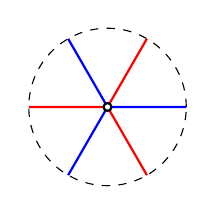
\begin{tikzpicture}
\begin{scope}
\draw[dashed] (0,0) circle (1cm);
\draw[red, thick] (60:1)--(0,0) (180:1)--(0,0) (-60:1)--(0,0);
\draw[blue, thick] (0:1)--(0,0) (120:1)--(0,0) (240:1)--(0,0);
\draw[thick,black,fill=white] (0,0) circle (0.05);
\end{scope}
\end{tikzpicture}
\caption{A hexagonal point}
\label{fig:hexagonal_point}
\end{figure}


Let $\pi_F:J^1S \cong T^*S\times\R\to S\times \R$ be the front projection, and we call the image $\pi_F(\Legendrian)$ of a Legendrian~$\Legendrian\subset J^1S$ a \emph{wavefront}.
Since $J^1S$ is equipped with the contact form $dz-p_x dx-p_y dy$, the coordinates~$(p_x,p_y)$ of the Legendrian $\Legendrian$ are recovered from $(x,y)$-slope of the tangent plane $T_{(x,y,z)}\pi_F(\Legendrian)$:
\begin{align*}
p_x&=\partial_x z(x,y),&  p_y&=\partial_y z(x,y).
\end{align*}
For any $N$-graph $\ngraph$ on a surface $S$, we associate a Legendrian surface $\Legendrian(\ngraph)\subset J^1S$. 
Basically, we construct the Legendrian surface by weaving the wavefronts in $S \times \R$ constructed from a local chart of $S$. 

Let $\ngraph\subset S$ be an $N$-graph.
A finite cover $\{U_i\}_{i\in I}$ of $S$ is called {\em $\ngraph$-compatible} if
\begin{enumerate}
\item each $U_i$ is diffeomorphic to the open disk $\mathring{\disk}^2$,
\item $U_i \cap \ngraph$ is connected, and
\item $U_i \cap \ngraph$ contains at most one vertex.
\end{enumerate}

For each $U_i$, we associate a wavefront $\wavefront(U_i)\subset U_i\times \R \subset S\times \R$.
Note that there are only five types of nondegenerate local charts for any $N$-graph $\ngraph$ as follows:
\begin{enumerate}[Type 1]
\item A chart without any graph component whose corresponding wavefront becomes
\[
\bigcup_{i=1,\dots,N}\mathring{\disk}^2\times\{i\}\subset \mathring{\disk}^2\times \R.
\]

\item A chart with single edge. The corresponding wavefront is the union of the $\dynA_1^2$-germ along the two sheets $\mathring\disk^2\times \{i\}$ and $\mathring\disk^2\times\{i+1\}$, and trivial disks $\disk^2\times\{j\}$, $j\in \{1,\dots,N\}\setminus\{i,i+1\}$.%\bhnote{$i\in \{1,\dots,N\}\setminus\{i,i+1\}$?}
The local model of $\dynA_1^2$ comes from the origin of the singular surface
\[
\wavefront(\dynA_1^2)=\{(x,y,z)\in \R^3 \mid x^2-z^2=0\}
\]
See Figure~\ref{fig:A_1^2 germ}.

\item A chart with transversely intersecting two edges. The wavefront consists of two $\dynA_1^2$-germs of $\mathring\disk^2\times\{i,i+1\}$ and $\mathring\disk^2\times\{j,j+1\}$, and trivial disks $\disk^2\times\{k\}$, $k\in \{1,\dots,N\}\setminus\{i,i+1,j,j+1\}$.

\item A chart with a monochromatic trivalent vertex whose wavefront is the union of the $\dynD_4^-$-germ, see \cite[\S2.4]{Arn1990}, and trivial disks $\disk^2\times\{j\}$, $j\in \{1,\dots,N\}\setminus\{i,i+1\}$.
The local model for Legendrian singularity of type $\dynD_4^-$ is given by the image at the origin of 
\begin{align*}
\delta_4^-:\R^2\to \R^3:(x,y)\mapsto \left( x^2-y^2, 2xy, \frac{2}{3}(x^3-3xy^2) \right).
\end{align*}
See Figure~\ref{fig:D_4^- germ}.

\item A chart with a bichromatic hexagonal point. The induced wavefront is the union of the $\dynA_1^3$-germ along the three sheets $\mathring\disk^2\times \{*\}$, $*=i,i+1,i+2$, and the trivial disks $\disk^2\times\{j\}$, $j\in \{1,\dots,N\}\setminus\{i,i+1,i+2\}$. The local model of $\dynA_1^3$ is given by the origin of the singular surface
\[
\{(x,y,z)\in \R^3 \mid (x^2-z^2)(y-z)=0\}.
\]
See Figure~\ref{fig:A_1^3 germ}.
\end{enumerate}


\begin{figure}[ht]
\subfigure[The germ of $A_1^2$\label{fig:A_1^2 germ}]{\makebox[0.3\textwidth]{$
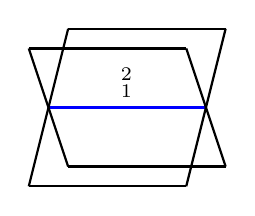
\begin{tikzpicture}[baseline=-.5ex,scale=1]
\begin{scope}
\draw[blue, thick] (-1,0)--(1,0) node[black,above, midway] {$\dynA_1^2$};
\draw[thick] (-3/4,1)--(5/4,1);
\draw[thick] (5/4,1)--(3/4,-1);
\draw[thick] (3/4,-1)--(-5/4,-1);
\draw[thick] (-5/4,-1)--(-3/4,1);
\draw[thick] (-5/4,3/4)--(3/4,3/4);
\draw[thick] (3/4,3/4)--(5/4,-3/4);
\draw[thick] (5/4,-3/4)--(-3/4,-3/4);
\draw[thick] (-3/4,-3/4)--(-5/4,3/4);
\end{scope}
\end{tikzpicture}
$}}
\subfigure[The germ of $A_1^3$\label{fig:A_1^3 germ}]{\makebox[0.3\textwidth]{$
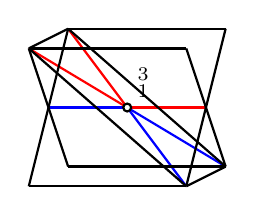
\begin{tikzpicture}[baseline=-.5ex,scale=1]
\begin{scope}
\draw[red, thick] (0,0)--(1,0);
\draw[red, thick] (-5/4,3/4)--(0,0);
\draw[red, thick] (-3/4,1)--(0,0);

\draw[blue, thick] (-1,0)--(0,0);
\draw[blue, thick] (0,0)--(5/4,-3/4);
\draw[blue, thick] (0,0)--(3/4,-1);

\draw[thick] (-3/4,1)--(5/4,1);
\draw[thick] (5/4,1)--(3/4,-1);
\draw[thick] (3/4,-1)--(-5/4,-1);
\draw[thick] (-5/4,-1)--(-3/4,1);
\draw[thick,black,fill=white] (0,0) circle (0.05) node[above right] {$\dynA_1^3$};
\draw[thick] (-5/4,3/4)--(3/4,3/4);
\draw[thick] (3/4,3/4)--(5/4,-3/4);
\draw[thick] (5/4,-3/4)--(-3/4,-3/4);
\draw[thick] (-3/4,-3/4)--(-5/4,3/4);

\draw[thick] (-5/4,3/4)--(-3/4,1);
\draw[thick] (-3/4,1)--(5/4,-3/4);
\draw[thick] (5/4,-3/4)--(3/4,-1);
\draw[thick] (3/4,-1)--(-5/4,3/4);
\end{scope}
\end{tikzpicture}
$}}
\subfigure[The germ of $D_4^-$\label{fig:D_4^- germ}]{\makebox[0.3\textwidth]{$
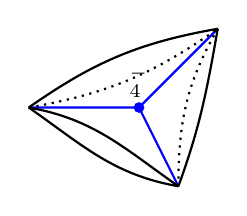
\begin{tikzpicture}[baseline=-.5ex,scale=1]
\begin{scope}
\draw[blue, thick, fill] (-1.4,0)--(0,0) circle (1.5pt);
\draw[blue, thick] (0,0)--(1,1);
\draw[blue, thick] (0,0)--(1/2,-1);
\node[above] at (0,0) {$\dynD_4^-$};

\draw[thick] (-1.4,0) to[out=35,in=190] (1,1);
\draw[dotted, thick] (-1.4,0) to[out=10,in=215] (1,1);

\draw[thick] (-1.4,0) to[out=-35,in=170] (1/2,-1);
\draw[thick] (-1.4,0) to[out=-10,in=145] (1/2,-1);

\draw[dotted,thick] (1/2,-1) to[out=90,in=240] (1,1);
\draw[thick] (1/2,-1) to[out=70,in=260] (1,1);
\end{scope}
\end{tikzpicture}
$}}

\caption{Three-types of wavefronts of Legendrian singularities.}
\label{fig:legendrian_singularities}
\end{figure}

\begin{figure}[ht]
\begin{tikzpicture}
\begin{scope}
\draw[thick] \boundellipse{0,1}{1.25}{0.25};

\draw[blue, thick] (-1,0)--(1,0);
\draw[thick] (-3/4,1/3)--(5/4,1/3);
\draw[thick] (5/4,1/3)--(3/4,-1/3);
\draw[thick] (3/4,-1/3)--(-5/4,-1/3);
\draw[thick] (-5/4,-1/3)--(-3/4,1/3);
\draw[thick] (-5/4,3/12)--(3/4,3/12);
\draw[thick] (3/4,3/12)--(5/4,-3/12);
\draw[thick] (5/4,-3/12)--(-3/4,-3/12);
\draw[thick] (-3/4,-3/12)--(-5/4,3/12);

\draw[thick] \boundellipse{0,-1}{1.25}{0.25};
\draw[thick] \boundellipse{0,-2}{1.25}{0.25};
\draw[blue, thick] (-5/4,-2)--(5/4,-2);
\draw[thick, ->] (0,-1.35)--(0,-1.9);

\node at (1.5,1){\tiny $N$};
\node at (0,2/3){\tiny $\vdots$};
\node at (1.5,1/3){\tiny $i+1$};
\node at (1.5,-1/3){\tiny $i$};
\node at (0,-0.45){\tiny $\vdots$};
\node at (1.5,-1){\tiny $1$};

\end{scope}

\begin{scope}[xshift=3.5cm]
%\draw[thick] \boundellipse{0,1}{1.25}{0.25};

\begin{scope}[yshift=0.6cm]
\draw[thick] (-5/4,-1/9)--(-1/4,1/3);
\draw[thick] (1/4,-1/9)--(5/4,1/3);
\draw[thick] (-5/4,-1/3)--(-1/4,1/9);
\draw[thick] (1/4,-1/3)--(5/4,1/9);
\draw[thick] (1/4,-1/3)--(-5/4,-1/9);
\draw[thick] (-5/4,-1/3)--(1/4,-1/9);
\draw[thick] (-1/4,1/9)--(5/4,1/3);
\draw[thick] (5/4,1/9)--(-1/4,1/3);
\draw[thick,yellow] (-1/2,-2/9)--(1/2,2/9);
\end{scope}

\begin{scope}[yshift=-0.75cm]
\draw[blue, thick] (-1,0)--(1,0);
\draw[thick] (-3/4,1/3)--(5/4,1/3);
\draw[thick] (5/4,1/3)--(3/4,-1/3);
\draw[thick] (3/4,-1/3)--(-5/4,-1/3);
\draw[thick] (-5/4,-1/3)--(-3/4,1/3);
\draw[thick] (-5/4,3/12)--(3/4,3/12);
\draw[thick] (3/4,3/12)--(5/4,-3/12);
\draw[thick] (5/4,-3/12)--(-3/4,-3/12);
\draw[thick] (-3/4,-3/12)--(-5/4,3/12);
\end{scope}

%\draw[thick] \boundellipse{0,-1}{1.25}{0.25};
\draw[thick] \boundellipse{0,-2}{1.25}{0.25};
\draw[blue, thick] (-5/4,-2)--(5/4,-2);
\draw[yellow, thick] (-0.6,-2-2/9)--(0.6,-2+2/9);
\draw[thick, ->] (0,-1.35)--(0,-1.9);

\node at (1.5,1){\tiny $j+1$};
\node at (1.5,1/3){\tiny $j$};
\node at (0,0){\tiny $\vdots$};
\node at (1.5,-1/3){\tiny $i+1$};
\node at (1.5,-1){\tiny $i$};

\end{scope}

\begin{scope}[xshift=7cm]
\draw[thick] \boundellipse{0,1}{1.25}{0.25};

\draw[blue, thick] (-1.25,0)--(0,0);
\draw[blue, thick] (0,0)--(1.25,1/3);
\draw[blue, thick] (0,0)--(1/2,-1/3);
\draw[thick,blue,fill=blue] (0,0) circle (0.05);

\draw[thick] (-1.25,0) to[out=25,in=175] (1.25,1/3);
\draw[dotted, thick] (-1.25,0) to[out=10,in=190] (1.25,1/3);

\draw[thick] (-1.25,0) to[out=-25,in=180] (1/2,-1/3);
\draw[thick] (-1.25,0) to[out=-10,in=160] (1/2,-1/3);

\draw[dotted,thick] (1/2,-1/3) to[out=80,in=220] (1.25,1/3);
\draw[thick] (1/2,-1/3) to[out=30,in=250] (1.25,1/3);

\draw[thick] \boundellipse{0,-1}{1.25}{0.25};
\draw[thick] \boundellipse{0,-2}{1.25}{0.25};
\draw[blue, thick] (-5/4,-2)--(0,-2);
\draw[blue, thick] (0,-2)--(0.90,-1.825);
\draw[blue, thick] (0,-2)--(1/2,-2.225);

\draw[thick,blue,fill=blue] (0,-2) circle (0.05);
\draw[thick, ->] (0,-1.35)--(0,-1.9);

\node at (1.5,1){\tiny $N$};
\node at (0,2/3){\tiny $\vdots$};
\node at (1.5,1/3){\tiny $i+1$};
\node at (1.5,-1/3){\tiny $i$};
\node at (0,-0.45){\tiny $\vdots$};
\node at (1.5,-1){\tiny $1$};

\end{scope}

\begin{scope}[xshift=10.5cm]
\draw[thick] \boundellipse{0,1}{1.25}{0.25};

\draw[red, thick] (0,0)--(1,0);
\draw[red, thick] (-5/4,3/12)--(0,0);
\draw[red, thick] (-3/4,1/3)--(0,0);

\draw[blue, thick] (-1,0)--(0,0);
\draw[blue, thick] (0,0)--(5/4,-3/12);
\draw[blue, thick] (0,0)--(3/4,-1/3);

\draw[thick] (-3/4,1/3)--(5/4,1/3);
\draw[thick] (5/4,1/3)--(3/4,-1/3);
\draw[thick] (3/4,-1/3)--(-5/4,-1/3);
\draw[thick] (-5/4,-1/3)--(-3/4,1/3);
\draw[thick,black,fill=white] (0,0) circle (0.05);
\draw[thick] (-5/4,3/12)--(3/4,3/12);
\draw[thick] (3/4,3/12)--(5/4,-3/12);
\draw[thick] (5/4,-3/12)--(-3/4,-3/12);
\draw[thick] (-3/4,-3/12)--(-5/4,3/12);

\draw[thick] (-5/4,3/12)--(-3/4,1/3);
\draw[thick] (-3/4,1/3)--(5/4,-3/12);
\draw[thick] (5/4,-3/12)--(3/4,-1/3);
\draw[thick] (3/4,-1/3)--(-5/4,3/12);


\draw[thick] \boundellipse{0,-1}{1.25}{0.25};
\draw[thick] \boundellipse{0,-2}{1.25}{0.25};
\draw[blue, thick] (-5/4,-2)--(0,-2);
\draw[blue, thick] (0,-2)--(0.90,-1.825);
\draw[blue, thick] (0,-2)--(1/2,-2.225);

\draw[red, thick] (5/4,-2)--(0,-2);
\draw[red, thick] (0,-2)--(-0.90,-2.175);
\draw[red, thick] (0,-2)--(-1/2,-1.775);
\draw[thick,black,fill=white] (0,-2) circle (0.05);

\draw[thick, ->] (0,-1.35)--(0,-1.9);

\node at (1.5,1){\tiny $N$};
\node at (0,2/3){\tiny $\vdots$};
\node at (1.5,1/3){\tiny $i+2$};
\node at (1.5,0){\tiny $i+1$};
\node at (1.5,-1/3){\tiny $i$};
\node at (0,-0.45){\tiny $\vdots$};
\node at (1.5,-1){\tiny $1$};

\end{scope}


\end{tikzpicture}
\caption{Local charts for $N$-graphs of Type 2,3,4, and 5.}
\label{fig:local_chart_3-graphs}
\end{figure}

\begin{definition}\cite[Definition~2.7]{CZ2020}
Let $\ngraph$ be an $N$-graph on a surface $S$. 
The {\em Legendrian weave}~$\Legendrian(\ngraph)\subset J^1 S$ is an embedded Legendrian surface whose wavefront $\wavefront(\ngraph)\subset S\times \R$ is constructed by weaving the wavefronts $\{\wavefront(U_i)\}_{i\in I}$ from a $\ngraph$-compatible cover $\{U_i\}_{i\in I}$ with respect to the gluing data given by $\ngraph$.
\end{definition}

\begin{remark}
Note that $\Legendrian(\ngraph)$ is well-defined up to the choice of cover and up to planar isotopies.
Let $\{\varphi_t\}_{t\in[0,1]}$ be a compactly supported isotopy of $S$.
Then this induces a Legendrian isotopy of Legendrian surface $\Legendrian(\varphi_t(\ngraph))\subset J^1 S$ relative to the boundary.
\end{remark}

We also list certain degenerate local models of $N$-graph as follows:
\begin{enumerate}[Type~D1]
\item A chart with double edges whose wavefront consists of two $\dynA_1^2$-germs of $\mathring\disk^2\times\{i,i+1\}$ and $\mathring\disk^2\times\{j,j+1\}$ for $|i-j|>1$, and trivial disks $\disk^2\times\{k\}$, $k\in \{1,\dots,N\}\setminus\{i,i+1,j,j+1\}$.
See Figure~\ref{fig:degenerate type1}.

\item A chart with trichromatic graph of $(\ngraph_{i-1},\ngraph_i,\ngraph_{i+1})$ satisfying \label{degenerate_type2}
\begin{itemize}
\item each has a unique vertex of four valent,
\item $\ngraph_{i-1}$ and $\ngraph_{i+1}$ are identical, and
\item $\ngraph_i$ and $\ngraph_{i+1}$ are intersecting at the vertex of eight valent in an alternating way, see the middle one in Figure~\ref{fig:degenerate type2}.
\end{itemize}
\end{enumerate}

For $i=2$, the wavefront corresponding to a chart of \ref{degenerate_type2} inside $\disk^2\times \R$ consists of four disks $(\disk_1,\dots,\disk_4)$, which is the cone $C(\legendrian)=\legendrian\times[0,1]/\legendrian\times\{0\}$ of the following Legendrian front $\legendrian$ in $\sphere^1\times\R$
\[
(\sigma_{1,3}\sigma_2)^4=\vcenter{\hbox{
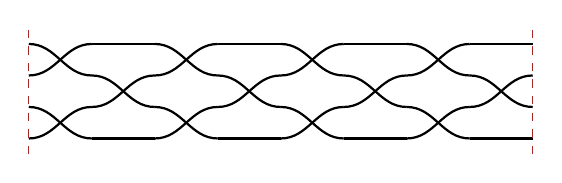
\begin{tikzpicture}[scale=0.8]
\begin{scope}
\foreach \x in {0,2,4,6}
{
\draw[thick] (\x,0) to[out=0,in=180] (\x+1,0.5);
\draw[thick] (\x,0.5) to[out=0,in=180] (\x+1,0);
}
\draw[thick] (1,0) -- (2,0) (3,0)--(4,0) (5,0)--(6,0) (7,0)--(8,-0);
\end{scope}
\begin{scope}[xshift=1cm,yshift=0.5cm]
\foreach \x in {0,2,4,6}
{
\draw[thick] (\x,0) to[out=0,in=180] (\x+1,0.5);
\draw[thick] (\x,0.5) to[out=0,in=180] (\x+1,0);
}
\end{scope}
\begin{scope}[yshift=1cm]
\foreach \x in {0,2,4,6}
{
\draw[thick] (\x,0) to[out=0,in=180] (\x+1,0.5);
\draw[thick] (\x,0.5) to[out=0,in=180] (\x+1,0);
}
\draw[thick] (1,0.5) -- (2,0.5) (3,0.5)--(4,0.5) (5,0.5)--(6,0.5) (7,0.5)--(8,0.5);
\end{scope}
\draw[red, dashed] (0,-0.25)--(0,1.75)  (8,-0.25)--(8,1.75);
\end{tikzpicture}
}},
\] 
where $\sigma_{1,3}$ is a $4$-braid isotopic to $\sigma_1\sigma_3$ (or equivalently, $\sigma_3\sigma_1$) such that two crossings $\sigma_1$ and $\sigma_3$ occur simultaneously. 

\begin{figure}[ht]
\subfigure[Type 1\label{fig:degenerate type1}]{
$\begin{tikzpicture}[baseline=-.5ex,scale=0.5]
\draw[dashed] (0,0) circle (3);
\clip (0,0) circle (3);
\draw[Dble={green and blue},line width=2] (-3,0) -- (0,0);
\draw[Dble={green and blue},line width=2] (3,0) -- (0,0);
\end{tikzpicture}
\stackrel{\text{perturb.}}{\longrightarrow}
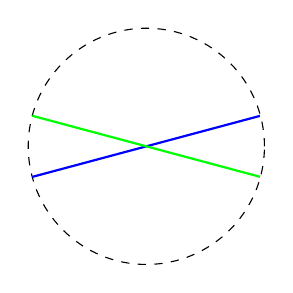
\begin{tikzpicture}[baseline=-.5ex,scale=0.5]
\draw[dashed] (0,0) circle (3);
\clip (0,0) circle (3);
\draw[thick, blue] (15:3) -- (15:-3);
\draw[thick, green] (-15:3) -- (-15:-3);
\end{tikzpicture}
\quad
\begin{tikzpicture}[baseline=-.5ex,scale=0.5]
\draw[dashed] (0,0) circle (3);
\clip (0,0) circle (3);
\draw[Dble={green and blue},line width=2] (120:3) -- (0,0);
\draw[Dble={green and blue},line width=2] (-120:3) -- (0,0);
\draw[Dble={green and blue},line width=2] (0,0) -- (3,0);
\end{tikzpicture}
\stackrel{\text{perturb.}}{\longrightarrow}
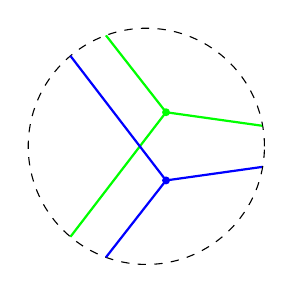
\begin{tikzpicture}[baseline=-.5ex,scale=0.5]
\draw[dashed] (0,0) circle (3);
\clip (0,0) circle (3);
\draw[thick, green, fill] (110:3) -- (60:1) circle (2pt) (-130:3) -- (60:1) (10:3) -- (60:1);
\draw[thick, blue, fill] (130:3) -- (-60:1) circle (2pt) (-110:3) -- (-60:1) (-10:3) -- (-60:1);
\end{tikzpicture}$
}

\subfigure[Type 2\label{fig:degenerate type2}]{
$
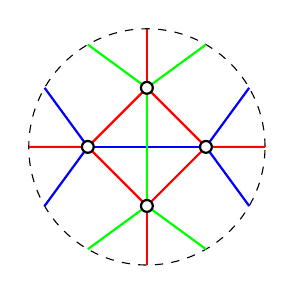
\begin{tikzpicture}[baseline=-.5ex,scale=1.5]
\draw [dashed] (0,0) circle [radius=1];

\draw [blue, thick] ({-sqrt(3)/2},1/2)--(-1/2,0);
\draw [blue, thick] ({-sqrt(3)/2},-1/2)--(-1/2,0);
\draw [blue, thick] ({sqrt(3)/2},1/2)--(1/2,0);
\draw [blue, thick] ({sqrt(3)/2},-1/2)--(1/2,0);
\draw [blue, thick] (-1/2,0)--(1/2,0);

\draw [red, thick] (-1,0)--(-1/2,0) to (0,1/2) to (1/2,0)--(1,0);
\draw [red, thick] (-1/2,0) to (0, -1/2) to (1/2,0); 
\draw [red, thick] (0,1) to (0,1/2);
\draw [red, thick] (0,-1) to (0,-1/2);

\draw [green, thick] (-1/2,{sqrt(3)/2}) to (0,1/2) to (0,-1/2) to (-1/2,-{sqrt(3)/2});
\draw [green, thick] (1/2,{sqrt(3)/2})--(0,1/2);
\draw [green, thick] (1/2,-{sqrt(3)/2})--(0,-1/2);


\draw[thick,black,fill=white] (-1/2,0) circle (0.05);
\draw[thick,black,fill=white] (1/2,0) circle (0.05);

\draw[thick,black,fill=white] (0,1/2) circle (0.05);
\draw[thick,black,fill=white] (0,-1/2) circle (0.05);
\end{tikzpicture}
\stackrel{\text{perturb.}}{\longleftarrow}
\begin{tikzpicture}[baseline=-.5ex,scale=0.5]
\draw[dashed] (0,0) circle (3);
\clip (0,0) circle (3);
\draw[fill, red, thick] 
(-3,0) -- (3,0) (0,3)--(0,-3);
\begin{scope}
\draw[Dble={blue and green},line width=2] (0,0) -- (-45:3);
\draw[Dble={green and blue},line width=2] (0,0) -- (45:3);
\draw[Dble={blue and green},line width=2] (0,0) -- (135:3);
\draw[Dble={green and blue},line width=2] (0,0) -- (-135:3);
\end{scope}
\end{tikzpicture}
=
\begin{tikzpicture}[baseline=-.5ex,scale=0.5]
\draw[dashed] (0,0) circle (3);
\clip (0,0) circle (3);
\draw[fill, red, thick] 
(-3,0) -- (3,0) (0,3)--(0,-3);
\begin{scope}
\draw[Dble={blue and green},line width=2] (-45:1.5) -- (0,0);
\draw[Dble={green and blue},line width=2] (45:1.5) -- (0,0);
\draw[Dble={blue and green},line width=2] (135:1.5) -- (0,0);
\draw[Dble={green and blue},line width=2] (-135:1.5) -- (0,0);
%
\draw[Dble={blue and green},line width=2] (-45:1.5) -- (-45:3);
\draw[Dble={green and blue},line width=2] (45:1.5) -- (45:3);
\draw[Dble={blue and green},line width=2] (135:1.5) -- (135:3);
\draw[Dble={green and blue},line width=2] (-135:1.5) -- (-135:3);
\end{scope}
\end{tikzpicture}
\stackrel{\text{perturb.}}{\longrightarrow}
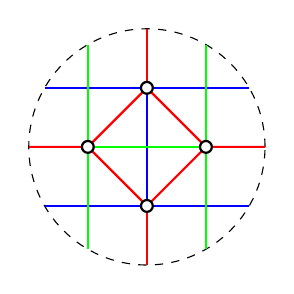
\begin{tikzpicture}[baseline=-.5ex,scale=1.5]
\draw [dashed] (0,0) circle [radius=1];
\draw [blue, thick] ({-sqrt(3)/2},1/2)--({+sqrt(3)/2},1/2);
\draw [blue, thick] ({-sqrt(3)/2},-1/2)--({+sqrt(3)/2},-1/2);
\draw [blue, thick] (0,1/2)--(0,-1/2);

\draw [red, thick] (-1,0)--(-1/2,0) to (0,1/2) to (1/2,0)--(1,0);
\draw [red, thick] (-1/2,0) to (0, -1/2) to (1/2,0); 
\draw [red, thick] (0,1) to (0,1/2);
\draw [red, thick] (0,-1) to (0,-1/2);

\draw [green, thick] (-1/2,{sqrt(3)/2}) to (-1/2,{-sqrt(3)/2});
\draw [green, thick] (1/2,{sqrt(3)/2}) to (1/2,{-sqrt(3)/2});
\draw [green, thick] (-1/2,0) to (1/2,0);


\draw[thick,black,fill=white] (-1/2,0) circle (0.05);
\draw[thick,black,fill=white] (1/2,0) circle (0.05);

\draw[thick,black,fill=white] (0,1/2) circle (0.05);
\draw[thick,black,fill=white] (0,-1/2) circle (0.05);
\end{tikzpicture}
$}
\caption{Local models for degenerate $N$-graphs and their perturbations}
\label{figure:perturbation of degenerated Ngraphs}
\end{figure}

\begin{remark}
The cone point neighborhood of the wavefront for the degenerate $N$-graph of~\ref{degenerate_type2}, is diffeomorphic to the union of four planes, $\{z=x\}, \{z=-x\}, \{z=y\},$ and $\{z=-y\}$ in $\R^3$, see Figure~\ref{fig:degenerated N-graph}.
Moreover, if we regard each of $\ngraph_i$ as a union of transversely intersecting two edges, then we have six edges for the local chart of $N$-graph $(\ngraph_1,\ngraph_2,\ngraph_3)$.
On the other hand, each pair of four disks in the wave front forms the $\dynA_1^2$-germ and this corresponds to the (degenerated) six edges.
\end{remark}


\begin{figure}[ht]
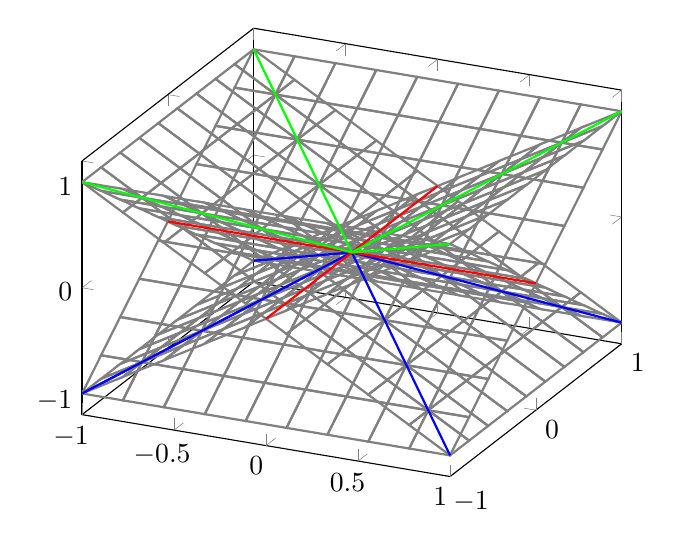
\begin{tikzpicture}
  \begin{axis}[domain=-1:1,y domain=-1:1]
     \draw[thick, blue] (0,0,0)--(-1,-1,-1);
    \addplot3[samples = 10,samples y = 10,mesh,draw = gray, thick] {x};
    \addplot3[samples = 10,samples y = 10,mesh,draw = gray, thick] {-x};
    \addplot3[samples = 10,samples y = 10,mesh,draw = gray, thick] {y};
    \addplot3[samples = 10,samples y = 10,mesh,draw = gray, thick] {-y};
\addplot3 [domain=-1:0, blue, thick] (x, x, x);
\addplot3 [domain=-1:0, blue, thick] (x, -x, x);
\addplot3 [domain=0:1, blue, thick] (x, x, -x);
\addplot3 [domain=0:1, blue, thick] (x, -x, -x);
\addplot3 [domain=-1:1, red, thick] (x, 0, 0);
\addplot3 [y domain=-1:1, red, thick] (0, y, 0);
\addplot3 [domain=-1:0, green, thick] (x, x, -x);
\addplot3 [domain=-1:0, green, thick] (x, -x, -x);
\addplot3 [domain=0:1, green, thick] (x, x, x);
\addplot3 [domain=0:1, green, thick] (x, -x, x);
  \end{axis}
\end{tikzpicture}
\caption{A wavefront for the degenerate $N$-graph.}
\label{fig:degenerated N-graph}
\end{figure}


We obtain (regular) $N$-graphs from degenerate $N$-graphs via (generic) perturbation of the wavefront as depicted in Figure~\ref{figure:perturbation of degenerated Ngraphs}.



The idea of $N$-graph is useful in the study of Legendrian surface, because the Legendrian isotopy of the Legendrian weave $\Legendrian(\ngraph)$ can be encoded in combinatorial moves of $N$-graphs.

\begin{theorem}\cite[Theorem~1.1]{CZ2020}\label{thm:N-graph moves and legendrian isotopy}
Let $\ngraph$ be a non-degenerate local $N$-graph. The combinatorial moves $\Move{I}\sim \Move{IV'}$ in Figure~\ref{fig:move1-6} are Legendrian isotopies for $\Legendrian(\ngraph)$.
\end{theorem}

We denote the equivalence class of an $N$-graph $\ngraph$ up to the moves $\Move{I}\sim \Move{IV'}$ in Figure~\ref{fig:move1-6} by~$[\ngraph]$.
Let us also list the combinatorial moves \Move{DI} and \Move{DII} for Legendrian isotopies involving degenerate $N$-graphs as depicted in Figure~\ref{fig:move1-6}.

\begin{corollary}
Let $\ngraph$ be a local degenerate $N$-graph. The combinatorial moves \Move{DI} and \Move{DII} in Figure~\ref{fig:move1-6} are Legendrian isotopies for $\Legendrian(\ngraph)$.
\end{corollary}

\begin{proof}
It is direct to check that the moves (DI) and (DII) for degenerate $N$-graphs can be obtained by composing the perturbations in Figure~\ref{figure:perturbation of degenerated Ngraphs} and moves in Figure~\ref{fig:move1-6}. See Appendix~\ref{appendix:DI and DII}.
\end{proof}



\begin{figure}[ht]
\begin{tikzpicture}
\begin{scope}%move_I
\draw [dashed] (0,0) circle [radius=1];%first circle
\draw [dashed] (3,0) circle [radius=1];%second circle
\draw [<->] (1.25,0) -- (1.75,0) node[midway, above] {\Move{I}};

\draw [blue, thick] ({-sqrt(3)/2},1/2)--(-1/2,0);
\draw [blue, thick] ({-sqrt(3)/2},-1/2)--(-1/2,0);
\draw [blue, thick] ({sqrt(3)/2},1/2)--(1/2,0);
\draw [blue, thick] ({sqrt(3)/2},-1/2)--(1/2,0);
\draw [blue, thick] (-1/2,0)--(1/2,0);

\draw [red, thick] (-1,0)--(-1/2,0) to[out=60,in=180] (0,1/2) to[out=0,in=120] (1/2,0)--(1,0);
\draw [red, thick] (-1/2,0) to[out=-60,in=180] (0, -1/2) to[out=0, in=-120] (1/2,0); 

\draw[thick,black,fill=white] (-1/2,0) circle (0.05);
\draw[thick,black,fill=white] (1/2,0) circle (0.05);

\draw [blue, thick] ({3-sqrt(3)/2},1/2)--({3+sqrt(3)/2},1/2);
\draw [blue, thick] ({3-sqrt(3)/2},-1/2)--({3+sqrt(3)/2},-1/2);
\draw [red, thick] (2,0)--(4,0);

\end{scope}

\begin{scope}[xshift=7cm]%move_II
\draw [dashed] (0,0) circle [radius=1];%first circle
\draw [dashed] (3,0) circle [radius=1];%second circle
\draw [<->] (1.25,0) -- (1.75,0) node[midway, above] {\Move{II}};

\draw [blue, thick] ({-sqrt(3)/2},1/2)--(-1/2,0);
\draw [blue, thick] ({-sqrt(3)/2},-1/2)--(-1/2,0);
\draw [blue, thick] ({sqrt(3)/2},1/2)--(1/2,0);
\draw [blue, thick] ({sqrt(3)/2},-1/2)--(1/2,0);
\draw [blue, thick] (-1/2,0)--(1/2,0);

\draw [red, thick] (-1/2,{sqrt(3)/2}) -- (1/2,0)--(1,0);
\draw [red, thick] (-1/2,{-sqrt(3)/2}) -- (1/2,0);

\draw[thick,blue,fill=blue] (-1/2,0) circle (0.05);
\draw[thick,black,fill=white] (1/2,0) circle (0.05);

\draw [blue, thick] ({3-sqrt(3)/2},1/2)--({3+sqrt(3)/2},1/2);
\draw [blue, thick] ({3-sqrt(3)/2},-1/2)--({3+sqrt(3)/2},-1/2);
\draw [blue, thick] (3,1/2)--(3,-1/2);

\draw [red, thick] (5/2,{sqrt(3)/2})--(3,1/2) to[out=-150,in=150] (3,-1/2)--(5/2,{-sqrt(3)/2});
\draw [red, thick] (3,1/2)--(7/2,0) -- (4,0);
\draw [red, thick] (3,-1/2)--(7/2,0);

\draw[thick,black,fill=white] (3,1/2) circle (0.05);
\draw[thick,black,fill=white] (3,-1/2) circle (0.05);
\draw[thick,red,fill=red] (7/2,0) circle (0.05);

\end{scope}

\begin{scope}[yshift=-2.5cm]%move_III_left
\draw [dashed] (0,0) circle [radius=1];
\draw [<->] (1.25,0) -- (1.75,0) node[midway, above] {\Move{III}};

\draw [blue, thick] ({-sqrt(3)/2},1/2)--(-1/2,0);
\draw [blue, thick] ({-sqrt(3)/2},-1/2)--(-1/2,0);
\draw [blue, thick] ({sqrt(3)/2},1/2)--(1/2,0);
\draw [blue, thick] ({sqrt(3)/2},-1/2)--(1/2,0);
\draw [blue, thick] (-1/2,0)--(1/2,0);

\draw [red, thick] (-1,0)--(-1/2,0) to[out=60,in=180] (0,1/2) to[out=0,in=120] (1/2,0)--(1,0);
\draw [red, thick] (-1/2,0) to[out=-60,in=180] (0, -1/2) to[out=0, in=-120] (1/2,0); 
\draw [red, thick] (0,1) to (0,1/2);
\draw [red, thick] (0,-1) to (0,-1/2);


\draw[thick,black,fill=white] (-1/2,0) circle (0.05);
\draw[thick,black,fill=white] (1/2,0) circle (0.05);

\draw[thick,red,fill=red] (0,1/2) circle (0.05);
\draw[thick,red,fill=red] (0,-1/2) circle (0.05);

\end{scope}

\begin{scope}[yshift=-2.5cm, xshift=3cm]%move_III_right

\draw [dashed] (0,0) circle [radius=1];

\draw [blue, thick] (-1/2,{sqrt(3)/2}) to (0,1/2) to (0,-1/2) to (-1/2,-{sqrt(3)/2});
\draw [blue, thick] (1/2,{sqrt(3)/2})--(0,1/2);
\draw [blue, thick] (1/2,-{sqrt(3)/2})--(0,-1/2);

\draw [red, thick] (-1,0)--(-1/2,0) to[out=60,in=180] (0,1/2) to[out=0,in=120] (1/2,0)--(1,0);
\draw [red, thick] (-1/2,0) to[out=-60,in=180] (0, -1/2) to[out=0, in=-120] (1/2,0); 
\draw [red, thick] (0,1) to (0,1/2);
\draw [red, thick] (0,-1) to (0,-1/2);


\draw[thick,red,fill=red] (-1/2,0) circle (0.05);
\draw[thick,red,fill=red] (1/2,0) circle (0.05);

\draw[thick,black,fill=white] (0,1/2) circle (0.05);
\draw[thick,black,fill=white] (0,-1/2) circle (0.05);
\end{scope}

\begin{scope}[xshift=7cm, yshift=-2.5cm]%move_IV_left
\draw [dashed] (0,0) circle [radius=1];
\draw [<->] (1.25,0) -- (1.75,0) node[midway, above] {\Move{IV}};

\draw [blue, thick] ({-sqrt(3)/2},1/2)--(-1/2,0);
\draw [blue, thick] ({-sqrt(3)/2},-1/2)--(-1/2,0);
\draw [blue, thick] ({sqrt(3)/2},1/2)--(1/2,0);
\draw [blue, thick] ({sqrt(3)/2},-1/2)--(1/2,0);
\draw [blue, thick] (-1/2,0)--(1/2,0);

\draw [red, thick] (-1,0)--(-1/2,0) to (0,1/2) to (1/2,0)--(1,0);
\draw [red, thick] (-1/2,0) to (0, -1/2) to (1/2,0); 
\draw [red, thick] (0,1) to (0,1/2);
\draw [red, thick] (0,-1) to (0,-1/2);

\draw [green, thick] (-1/2,{sqrt(3)/2}) to (0,1/2) to (0,-1/2) to (-1/2,-{sqrt(3)/2});
\draw [green, thick] (1/2,{sqrt(3)/2})--(0,1/2);
\draw [green, thick] (1/2,-{sqrt(3)/2})--(0,-1/2);


\draw[thick,black,fill=white] (-1/2,0) circle (0.05);
\draw[thick,black,fill=white] (1/2,0) circle (0.05);

\draw[thick,black,fill=white] (0,1/2) circle (0.05);
\draw[thick,black,fill=white] (0,-1/2) circle (0.05);

\end{scope}

\begin{scope}[xshift=10cm, yshift=-2.5cm]%move_IV_right
\draw [dashed] (0,0) circle [radius=1];
\draw [blue, thick] ({-sqrt(3)/2},1/2)--({+sqrt(3)/2},1/2);
\draw [blue, thick] ({-sqrt(3)/2},-1/2)--({+sqrt(3)/2},-1/2);
\draw [blue, thick] (0,1/2)--(0,-1/2);

\draw [red, thick] (-1,0)--(-1/2,0) to (0,1/2) to (1/2,0)--(1,0);
\draw [red, thick] (-1/2,0) to (0, -1/2) to (1/2,0); 
\draw [red, thick] (0,1) to (0,1/2);
\draw [red, thick] (0,-1) to (0,-1/2);

\draw [green, thick] (-1/2,{sqrt(3)/2}) to (-1/2,{-sqrt(3)/2});
\draw [green, thick] (1/2,{sqrt(3)/2}) to (1/2,{-sqrt(3)/2});
\draw [green, thick] (-1/2,0) to (1/2,0);


\draw[thick,black,fill=white] (-1/2,0) circle (0.05);
\draw[thick,black,fill=white] (1/2,0) circle (0.05);

\draw[thick,black,fill=white] (0,1/2) circle (0.05);
\draw[thick,black,fill=white] (0,-1/2) circle (0.05);

\end{scope}

\begin{scope}[xshift=0cm, yshift=-5cm]%move_V_left
\draw [dashed] (0,0) circle [radius=1];
\draw [<->] (1.25,0) -- (1.75,0) node[midway, above] {\Move{V}};

\draw [blue, thick] ({-sqrt(3)/2},1/2)to[out=0,in=180](0,-1/2);
\draw [blue, thick] ({sqrt(3)/2},1/2)to[out=180,in=0](0,-1/2);

\draw [yellow, thick] ({-sqrt(3)/2},-1/2)to[out=0,in=180](0,1/2);
\draw [yellow, thick] ({sqrt(3)/2},-1/2)to[out=180,in=0](0,1/2);

\end{scope}

\begin{scope}[xshift=3cm, yshift=-5cm]%move_V_right
\draw [dashed] (0,0) circle [radius=1];

\draw [blue, thick] ({-sqrt(3)/2},1/2) to ({sqrt(3)/2},1/2);

\draw [yellow, thick] ({-sqrt(3)/2},-1/2) to ({sqrt(3)/2},-1/2);
\end{scope}

\begin{scope}[xshift=7cm, yshift=-5cm]%move_VI_left
\draw [dashed] (0,0) circle [radius=1];
\draw [<->] (1.25,0) -- (1.75,0) node[midway, above] {\Move{VI}};
\draw [blue, thick] ({-sqrt(3)/2},1/2) to (0,0) to(1,0);
\draw [blue, thick] ({-sqrt(3)/2},-1/2) to (0,0);

\draw[thick,blue,fill=blue] (0,0) circle (0.05);

\draw[yellow, thick] (0,1) to[out=-135,in=135] (0,-1);
\end{scope}

\begin{scope}[xshift=10cm, yshift=-5cm]%move_VI_right
\draw [dashed] (0,0) circle [radius=1];
\draw [blue, thick] ({-sqrt(3)/2},1/2) to (0,0) to(1,0);
\draw [blue, thick] ({-sqrt(3)/2},-1/2) to (0,0);

\draw[thick,blue,fill=blue] (0,0) circle (0.05);

\draw[yellow, thick] (0,1) to[out=-45,in=45] (0,-1);
\end{scope}

\begin{scope}[xshift=0cm, yshift=-7.5cm]%move_VI'_left
\draw [dashed] (0,0) circle [radius=1];
\draw [<->] (1.25,0) -- (1.75,0) node[midway, above] {\Move{VI'}};
\draw [blue, thick] ({-1/2},{sqrt(3)/2}) to (0,0) to(1,0);
\draw [blue, thick] ({-1/2},{-sqrt(3)/2}) to (0,0);

\draw [red, thick] (-1,0) to (0,0) to(1/2,{sqrt(3)/2});
\draw [red, thick] (0,0) to(1/2,{-sqrt(3)/2});

\draw[thick,black,fill=white] (0,0) circle (0.05);

\draw[yellow, thick] (0,1) to[out=-135,in=135] (0,-1);
\end{scope}

\begin{scope}[xshift=3cm, yshift=-7.5cm]%move_VI'_right
\draw [dashed] (0,0) circle [radius=1];
\draw [blue, thick] ({-1/2},{sqrt(3)/2}) to (0,0) to(1,0);
\draw [blue, thick] ({-1/2},{-sqrt(3)/2}) to (0,0);

\draw [red, thick] (-1,0) to (0,0) to(1/2,{sqrt(3)/2});
\draw [red, thick] (0,0) to(1/2,{-sqrt(3)/2});

\draw[thick,black,fill=white] (0,0) circle (0.05);

\draw[yellow, thick] (0,1) to[out=-45,in=45] (0,-1);
\end{scope}



\begin{scope}[xshift=0cm, yshift=-10cm]
\draw [dashed] (0,0) circle [radius=1];%first circle
\draw[red, thick] (160:1)--(-0.5,0) -- (1,0) (200:1)--(-0.5,0) (0,1)--(0,-1);
\draw[thick,red] (-1/2,0) circle (1pt);
\draw[Dble={blue and green},line width=2] (0,0) -- (-45:1);
\draw[Dble={green and blue},line width=2] (0,0) -- (45:1);
\draw[Dble={blue and green},line width=2] (0,0) -- (135:1);
\draw[Dble={green and blue},line width=2] (0,0) -- (-135:1);

\draw [<->] (1.25,0) -- (1.75,0) node[midway, above] {\Move{DI}};
\end{scope}

\begin{scope}[xshift=3cm, yshift=-10cm]
\draw [dashed] (0,0) circle [radius=1];%second circle
\clip (0,0) circle [radius=1];
\draw[rounded corners,thick, red](0,1)--(0,-1) (150:1)--++(5/4,0)--(3/4,0) (210:1)--++(5/4,0)--(3/4,0) (3/4,0)--(1,0);
\draw[Dble={green and blue},line width=2] (120:1) -- (0,0.5);
\draw[Dble={blue and green},line width=2] (60:1) -- (0,0.5);
\draw[Dble={blue and green},line width=2] (-120:1) -- (0,-0.5);
\draw[Dble={green and blue},line width=2] (-60:1) -- (0,-0.5);
\draw[blue,line width=2] (-0.05,0.5) to[out=-135,in=135] (-0.05,-0.5);
\draw[green,line width=2] (0,0.45) to[out=-135,in=135] (0,-0.45);
\draw[blue,line width=2] (0.05,0.5) to[out=-45,in=45] (0.05,-0.5);
\draw[green,line width=2] (0,0.45) to[out=-45,in=45] (0,-0.45);
\draw[thick,red,fill=red] (3/4,0) circle (1pt);
\end{scope}

\begin{scope}[xshift=7cm, yshift=-10cm]%move_II
\draw [<->] (1.25,0) -- (1.75,0) node[midway, above] {\Move{DII}};
\draw [dashed] (0,0) circle [radius=1];%first circle
\clip (0,0) circle [radius=1];
\draw[thick, red](135:1)--(-45:1) (45:1)--(-135:1);
\draw[Dble={blue and green},line width=2] (0,0) -- (-90:1);
\draw[Dble={blue and green},line width=2] (0,0) -- (90:1);
\draw[Dble={green and blue},line width=2] (0,0) -- (1,0);
\draw[Dble={green and blue},line width=2] (0,0) -- (-0.5,0);
\draw[Dble={green and blue},line width=2] (-0.5,0) -- (155:1.2);
\draw[Dble={green and blue},line width=2] (-0.5,0) -- (205:1.2);
\end{scope}

\begin{scope}[xshift=10cm, yshift=-10cm]
\draw [dashed] (0,0) circle [radius=1];%second circle
\clip (0,0) circle [radius=1];
\draw[thick, red](120:1)--(0,0.5) to[out=-45,in=45] (0,-0.5) --(-120:1)
(60:1)--(0,0.5) to[out=-135,in=135] (0,-0.5) --(-60:1);
\draw[Dble={green and blue},line width=2] (0,0.5) -- ++(-1,0);
\draw[Dble={green and blue},line width=2] (0,0.5) -- (0.3,0.5);
\draw[Dble={green and blue},line width=2] (0,1) -- (0,0.5);
\draw[Dble={green and blue},line width=2] (0,0) -- (0,0.5);
\draw[Dble={green and blue},line width=2] (0,0) -- (0,-0.5);
\draw[Dble={green and blue},line width=2] (0,-0.5) -- ++(-1,0);
\draw[Dble={green and blue},line width=2] (0,-0.5) -- (0.3,-0.5);
\draw[Dble={green and blue},line width=2] (0,-1) -- (0,-0.5);
\draw[blue,line width=2]
(0.3,-0.535) to[out=0,in=-135] (0.7,-0.035) 
(0.3,0.465) to[out=0,in=135] (0.7,-0.035) -- (1,-0.035);
\draw[green,line width=2]
(0.3,-0.465) to[out=0,in=-135] (0.7,0.035) 
(0.3,0.535) to[out=0,in=135] (0.7,0.035) -- (1,0.035);
\end{scope}
\end{tikzpicture}
\caption{Combinatorial moves for Legendrian isotopies of surface $\Legendrian(\ngraph)$.
Here the pairs ({\color{blue} blue}, {\color{red} red}) and ({\color{red} red}, {\color{green} green}) are consecutive. Other pairs are not.}
\label{fig:move1-6}
\end{figure}

\begin{definition}\label{definiton:freeness}
An $N$-graph $\ngraph$ on $S$ is called {\em free} if the induced Legendrian weave $\Legendrian(\ngraph)\subset J^1S$ can be woven without interior Reeb chord. 
\end{definition}

\begin{example}\cite[Example 7.3]{CZ2020}\label{ex:free N-graph}
Let $\ngraph\subset \disk^2$ be a $2$-graph such that $\disk^2\setminus \ngraph$ is simply connected relative to the boundary $\boundary\disk^2\cap(\disk^2\setminus \ngraph)$. Then $\ngraph$ is free if and only if $\ngraph$ has no faces contained in~$\mathring\disk^2$.
Note that each of such faces admits at least one Reeb chord, see Figure~\ref{fig:N-graphs with Reeb chords}.
\end{example}

\begin{figure}[ht]
\begin{tikzcd}
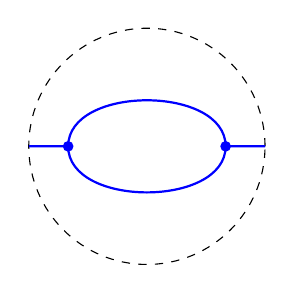
\begin{tikzpicture}
\draw [dashed] (0,0) circle [radius=1.5];
\draw [thick,blue] (-1.5,0)-- (-1,0) to[out=90,in=90] (1,0)--(1.5,0) (-1,0) to[out=-90,in=-90] (1,0);
\draw [thick, blue, fill] (-1,0) circle (1.5pt)  (1,0) circle (1.5pt);
\end{tikzpicture}
&
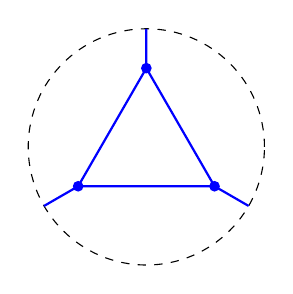
\begin{tikzpicture}
\draw [dashed] (0,0) circle [radius=1.5];
\draw [thick,blue] (90:1.5) -- (90:1) (210:1.5) -- (210:1) (-30:1.5) -- (-30:1)
(90:1) -- (210:1) -- (-30:1)-- (90:1);
\draw [thick, blue, fill] (90:1) circle (1.5pt) (210:1) circle (1.5pt) (-30:1) circle (1.5pt);
\end{tikzpicture}
\end{tikzcd}
\caption{$N$-graphs with Reeb chords}
\label{fig:N-graphs with Reeb chords}
\end{figure}


In particular, we have the following lemma whose proof is omitted.
\begin{lemma}\label{lemma:tree Ngraphs are free}
Let $\ngraph=(\ngraph_1,\dots,\ngraph_{N-1})$ be an $N$-graph on $\disk^2$. Suppose that each $\ngraph_i$ is a tree or empty. Then $\ngraph$ is free.
\end{lemma}
\begin{comment}
\begin{proof}
Recall from Definition~\ref{def:free} that an $3$-graph $\ngraph(a,b,c)$ is free if the Legendrian weave $\Legendrian(\ngraph(a,b,c))$ can be woven without Reeb chords. 
To investigate the Reeb chords of $\Legendrian(\ngraph(a,b,c))$ in $J^1\disk^2$,
let us consider the wavefront $\wavefront(\ngraph(a,b,c))$ in $\disk^2\times \R$.
Label the sheets of the wavefront 
\begin{equation}\label{equation:wavefront decomposition}
\wavefront(\ngraph(a,b,c))=\bigcup_{i=1}^{3}\wavefront_i
\end{equation}
by the $z$-coordinate from bottom to top. Let $f_i:\disk^2\to \R$ be a function whose graph becomes $\wavefront_i$, and let $h_{ij}:\disk^2\to \R$ be a difference function given by $f_j-f_i$ for any $1\le i<j\le 3$.
By the construction $h_{i\, i+1}^{-1}(0)$ gives the subgraph $\ngraph_i(a,b,c)$ of $\ngraph(a,b,c)=(\ngraph_1, \ngraph_2)$. 
The critical points of $h_{ij}$ on $\mathring{\disk}^2\setminus \ngraph(a,b,c)$ are the possible candidates for the Reeb chords. 
In other words, to guarantee that $\ngraph(a,b,c)$ is free, it suffices to show that $h_{ij}$ has no critical point on $\mathring{\disk}^2\setminus \ngraph(a,b,c)$. 

Let us analyze local configurations of gradients $\nabla h_{12}$, $\nabla h_{23}$.
\begin{enumerate}
\item Near the edge of $N$-graphs, the followings are examples of local configuration of $\nabla h_{12}$, $\nabla h_{23}$ depending on slope of Legendrian sheets. 
\[
\begin{tikzpicture}
\begin{scope}
\draw[thick] \boundellipse{0,1}{1.25}{0.25};

\draw[blue, thick] (-1,0)--(1,0);
\draw[thick] (-3/4,1/3)--(5/4,1/3);
\draw[thick] (5/4,1/3)--(3/4,-1/3);
\draw[thick] (3/4,-1/3)--(-5/4,-1/3);
\draw[thick] (-5/4,-1/3)--(-3/4,1/3);
\draw[thick] (-5/4,3/12)--(3/4,3/12);
\draw[thick] (3/4,3/12)--(5/4,-3/12);
\draw[thick] (5/4,-3/12)--(-3/4,-3/12);
\draw[thick] (-3/4,-3/12)--(-5/4,3/12);

\draw[thick] \boundellipse{0,-1}{1.25}{0.25};
\draw[blue, thick] (-5/4,-1)--(5/4,-1);
\draw[thick, ->] (0,-0.35)--(0,-0.9);

\node at (-1.5,1){\tiny $3$};
%\node at (0,2/3){\tiny $\vdots$};
\node at (-1.5,1/3){\tiny $2$};
\node at (-1.5,-1/3){\tiny $1$};
%\node at (0,-0.45){\tiny $\vdots$};
%\node at (-1.5,-1){\tiny $1$};

\end{scope}
\begin{scope}[xshift=10.5cm,decoration={markings, mark=at position 0.5 with {\arrow{>}}}]
\draw[thick] (0,0) circle (1cm);
\draw[blue, thick, dashed, opacity=0.5] (-1,0)--(1,0);
\node at (0,-1.5) {$\nabla h_{23}$};
%\draw[postaction={decorate}] (15:1) -- (0.8,0);
\draw[postaction={decorate}] (30:1) -- (0.5,0);
%\draw[postaction={decorate}] (45:1) -- (0.2,0);
\draw[postaction={decorate}] (60:1) -- (-0.1,0);
\draw[postaction={decorate}] (90:1) -- (-0.6,0);
\draw[postaction={decorate}] (120:1) -- (-1,0);
\draw[postaction={decorate}] (60:1) -- (-0.1,0);
%\draw[postaction={decorate}] (-15:1) -- (0.8,0);
\draw[postaction={decorate}] (-30:1) -- (0.5,0);
%\draw[postaction={decorate}] (-45:1) -- (0.2,0);
\draw[postaction={decorate}] (-60:1) -- (-0.1,0);
\draw[postaction={decorate}] (-90:1) -- (-0.6,0);
\draw[postaction={decorate}] (-120:1) -- (-1,0);
\end{scope}

\begin{scope}[xshift=7cm,decoration={markings, mark=at position 0.5 with {\arrow{>}}}]
\draw[thick] (0,0) circle (1cm);
\draw[blue, thick, dashed, opacity=0.5] (-1,0)--(1,0);
\node at (0,-1.5) {$\nabla h_{23}$};
%\draw[postaction={decorate}] (15:1) -- (0.8,0);
\draw[postaction={decorate}] (30:1) -- (0.5,0);
%\draw[postaction={decorate}] (45:1) -- (0.2,0);
\draw[postaction={decorate}] (60:1) -- (-0.1,0);
\draw[postaction={decorate}] (90:1) -- (-0.6,0);
\draw[postaction={decorate}] (120:1) -- (-1,0);
\draw[postaction={decorate}] (60:1) -- (-0.1,0);
%\draw[postaction={decorate}] (-15:1) -- (0.8,0);
\draw[postaction={decorate}]  (0.5,0) -- (-150:1);
%\draw[postaction={decorate}] (-45:1) -- (0.2,0);
\draw[postaction={decorate}] (-0.1,0) -- (-160:1);
\draw[postaction={decorate}] (-0.6,0) -- (-170:1);
\draw[postaction={decorate}] (1,0) -- (-140:1);
\draw[postaction={decorate}] (-20:1) -- (-120:1);
\end{scope}


\begin{scope}[xshift=3.5cm,decoration={markings, mark=at position 0.5 with {\arrow{>}}}]
\draw[thick] (0,0) circle (1cm);
\draw[blue, thick] (-1,0)--(1,0);
\node at (0,-1.5) {$\nabla h_{12}$};
\draw[postaction={decorate}] (1.732*0.5,0) -- (30:1);
\draw[postaction={decorate}] (0.5,0) -- (60:1);
\draw[postaction={decorate}] (0,0) -- (90:1);
\draw[postaction={decorate}] (-0.5,0) -- (120:1);
\draw[postaction={decorate}] (-1.732*0.5,0) -- (150:1);
\draw[postaction={decorate}] (1.732*0.5,0) -- (-30:1);
\draw[postaction={decorate}] (0.5,0) -- (-60:1);
\draw[postaction={decorate}] (0,0) -- (-90:1);
\draw[postaction={decorate}] (-0.5,0) -- (-120:1);
\draw[postaction={decorate}] (-1.732*0.5,0) -- (-150:1);
\end{scope}

\end{tikzpicture}
\]
Note that $\nabla h_{12}$, $\nabla h_{23}$ are not defined on the edge. 
Let $A$ and $B$ be two connected components of edge complement in the above neighborhood.
Then $\nabla h_{12}|_A$ and $(\nabla h_{12}+\nabla h_{23})|_B$ can be extended to the edge smoothly. 
This is because the $z$-coordinate differences among the three Legendrian sheets are smooth.

\item For the trivalent vertices in $\ngraph_2$, we consider the following gradient vector field configurations:
\[
\begin{tikzpicture}
\begin{scope}
\draw[thick] \boundellipse{0,1}{1.25}{0.25};

\draw[blue, thick] (-1.25,0)--(0,0);
\draw[blue, thick] (0,0)--(1.25,1/3);
\draw[blue, thick] (0,0)--(1/2,-1/3);
\draw[thick,blue,dashed,fill=blue] (0,0) circle (0.05);

\draw[thick] (-1.25,0) to[out=25,in=175] (1.25,1/3);
\draw[dotted, thick] (-1.25,0) to[out=10,in=190] (1.25,1/3);

\draw[thick] (-1.25,0) to[out=-25,in=180] (1/2,-1/3);
\draw[thick] (-1.25,0) to[out=-10,in=160] (1/2,-1/3);

\draw[dotted,thick] (1/2,-1/3) to[out=80,in=220] (1.25,1/3);
\draw[thick] (1/2,-1/3) to[out=30,in=250] (1.25,1/3);

\draw[thick] \boundellipse{0,-1}{1.25}{0.25};
%\draw[thick] \boundellipse{0,-2}{1.25}{0.25};
\draw[blue, thick] (-5/4,-1)--(0,-1);
\draw[blue, thick] (0,-1)--(0.90,-0.825);
\draw[blue, thick] (0,-1)--(1/2,-1.225);

\draw[thick,blue,fill=blue] (0,-1) circle (0.05);
\draw[thick, ->] (0,-0.35)--(0,-0.9);

\node at (-1.5,1){\tiny $3$};
%\node at (0,2/3){\tiny $\vdots$};
\node at (-1.5,1/3){\tiny $2$};
\node at (-1.5,-1/3){\tiny $1$};
%\node at (0,-0.45){\tiny $\vdots$};
%\node at (-1.5,-1){\tiny $1$};

\end{scope}


\begin{scope}[xshift=7cm,decoration={markings, mark=at position 0.5 with {\arrow{>}}}]
\draw[thick] (0,0) circle (1cm);
\draw[thick, blue, dashed, fill=blue, opacity=0.5] (0,0) circle (2pt) -- (60:1) (0,0) -- (-60:1) (0,0) -- (180:1);
\draw[postaction={decorate}] (170:1) -- (-0.5,0);
\draw[postaction={decorate}] (160:1) -- (0,0);
\draw[postaction={decorate}] (140:1) -- (60:0.5);
\draw[postaction={decorate}] (-170:1) -- (-0.5,0);
\draw[postaction={decorate}] (-160:1) -- (0,0);
\draw[postaction={decorate}] (-140:1) -- (-60:0.5);
\draw[postaction={decorate}] (60:0.5) -- (25:1);
\draw[postaction={decorate}] (-60:0.5) -- (-25:1);
\draw[postaction={decorate}] (0,0) -- (1,0);
\node at (0,-1.5) {$\nabla h_{23}$};
\end{scope}

%\begin{scope}[xshift=7cm,decoration={markings, mark=at position 0.5 with {\arrow{>}}}]
%\draw[thick] (0,0) circle (1cm);
%\draw[thick, red, fill=red, dashed, opacity=0.5] (0,0) circle (2pt) -- (60:1) (0,0) -- (-60:1) (0,0) -- (180:1);
%\draw[postaction={decorate}] (25:1) -- (60:0.5);
%\draw[postaction={decorate}] (-25:1) -- (-60:0.5);
%\draw[postaction={decorate}] (1,0) -- (0,0);
%\draw[postaction={decorate}] (60:0.5) -- (-0.5,0);
%\draw[postaction={decorate}] (-60:0.5) -- (-0.5,0);
%\draw[postaction={decorate}] (60:1) -- (-1,0);
%\draw[postaction={decorate}] (-60:1) -- (-1,0);
%\draw[postaction={decorate}] (90:1) -- (150:1);
%\draw[postaction={decorate}] (-90:1) -- (-150:1);
%\node at (0,-1.5) {$\nabla h_{12}, \nabla h_{34}$};
%\end{scope}

\begin{scope}[xshift=3.5cm,decoration={markings, mark=at position 0.5 with {\arrow{>}}}]
\draw[thick] (0,0) circle (1cm);
\draw[thick, blue, fill=blue] (0,0) circle (2pt) -- (60:1) (0,0) -- (-60:1) (0,0) -- (180:1);
\begin{scope}
\draw[postaction={decorate}] (0,0) -- (1,0);
\draw[postaction={decorate}] (60:0.5) to[out=-30,in=180] (15:1);
\draw[postaction={decorate}] (-60:0.5) to[out=30,in=180] (-15:1);
\end{scope}
\begin{scope}[rotate=120]
\draw[postaction={decorate}] (0,0) -- (1,0);
\draw[postaction={decorate}] (60:0.5) to[out=-30,in=180] (15:1);
\draw[postaction={decorate}] (-60:0.5) to[out=30,in=180] (-15:1);
\end{scope}
\begin{scope}[rotate=240]
\draw[postaction={decorate}] (0,0) -- (1,0);
\draw[postaction={decorate}] (60:0.5) to[out=-30,in=180] (15:1);
\draw[postaction={decorate}] (-60:0.5) to[out=30,in=180] (-15:1);
\end{scope}
\node at (0,-1.5) {$\nabla h_{12}$};
\end{scope}

\end{tikzpicture}
\]

\item Near the hexagonal point, we consider the following model of gradient vector fields.
\[
\begin{tikzpicture}
\begin{scope}
%\draw[thick] \boundellipse{0,1}{1.25}{0.25};

\begin{scope}[yshift=0.5cm,yscale=2]
\draw[red, thick] (0,0)--(1,0) (-5/4,3/12)--(0,0) (-3/4,1/3)--(0,0);

\draw[blue, thick] (-1,0)--(0,0) (0,0)--(5/4,-3/12) (0,0)--(3/4,-1/3);

\draw[thick] (-3/4,1/3)--(5/4,1/3);
\draw[thick] (5/4,1/3)--(3/4,-1/3);
\draw[thick] (3/4,-1/3)--(-5/4,-1/3);
\draw[thick] (-5/4,-1/3)--(-3/4,1/3);
\draw[thick] (-5/4,3/12)--(3/4,3/12);
\draw[thick] (3/4,3/12)--(5/4,-3/12);
\draw[thick] (5/4,-3/12)--(-3/4,-3/12);
\draw[thick] (-3/4,-3/12)--(-5/4,3/12);

\draw[thick] (-5/4,3/12)--(-3/4,1/3);
\draw[thick] (-3/4,1/3)--(5/4,-3/12);
\draw[thick] (5/4,-3/12)--(3/4,-1/3);
\draw[thick] (3/4,-1/3)--(-5/4,3/12);
\end{scope}
\draw[thick,black,fill=white] (0,0.5) circle (2pt);

\begin{scope}[yshift=0cm]
\draw[thick] \boundellipse{0,-1}{1.25}{0.25};
\draw[blue, thick] (-5/4,-1)--(0,-1) (0,-1)--(0.90,-0.825) (0,-1)--(1/2,-1.225);

\draw[red, thick] (5/4,-1)--(0,-1) (0,-1)--(-0.90,-1.175) (0,-1)--(-1/2,-0.775);
\draw[thick,black,fill=white] (0,-1) circle (2pt);

\draw[thick, ->] (0,-0.35)--(0,-0.9);
\end{scope}

%\node at (-1.5,1){\tiny $4$};
\node at (-1.5,1){\tiny $3$};
\node at (-1.5,0.5){\tiny $2$};
\node at (-1.5,0){\tiny $1$};
\end{scope}

\begin{scope}[xshift=3.5cm,decoration={markings, mark=at position 0.5 with {\arrow{>}}}]
\draw[thick] (0,0) circle (1cm);
\draw[thick, blue] (0,0)-- (60:1) (0,0)--(180:1) (0,0)--(-60:1);
\draw[thick, red, dashed, opacity=0.5] (0,0)-- (1,0) (0,0)--(120:1) (0,0)--(-120:1);
\draw[thick,black,fill=white] (0,0) circle (2pt);
\begin{scope}
\draw[postaction={decorate}] (60:0.25) to (0:0.5);
\draw[postaction={decorate}] (-60:0.25) to (0:0.5);
\draw[postaction={decorate}] (60:0.5) to (0:1);
\draw[postaction={decorate}] (-60:0.5) to (0:1);
\draw[postaction={decorate}] (60:0.75) to (20:1);
\draw[postaction={decorate}] (-60:0.75) to (-20:1);
\end{scope}
\begin{scope}[rotate=120]
\draw[postaction={decorate}] (60:0.25) to (0:0.5);
\draw[postaction={decorate}] (-60:0.25) to (0:0.5);
\draw[postaction={decorate}] (60:0.5) to (0:1);
\draw[postaction={decorate}] (-60:0.5) to (0:1);
\draw[postaction={decorate}] (60:0.75) to (20:1);
\draw[postaction={decorate}] (-60:0.75) to (-20:1);
\end{scope}
\begin{scope}[rotate=240]
\draw[postaction={decorate}] (60:0.25) to (0:0.5);
\draw[postaction={decorate}] (-60:0.25) to (0:0.5);
\draw[postaction={decorate}] (60:0.5) to (0:1);
\draw[postaction={decorate}] (-60:0.5) to (0:1);
\draw[postaction={decorate}] (60:0.75) to (20:1);
\draw[postaction={decorate}] (-60:0.75) to (-20:1);
\end{scope}
\node at (0,-1.5) {$\nabla h_{12}$};
\end{scope}

\begin{scope}[xshift=7cm,decoration={markings, mark=at position 0.5 with {\arrow{>}}}]
\draw[thick] (0,0) circle (1cm);
\draw[thick, blue, dashed, opacity=0.5] (0,0)-- (60:1) (0,0)--(180:1) (0,0)--(-60:1);
\draw[thick, red] (0,0)-- (1,0) (0,0)--(120:1) (0,0)--(-120:1);
\draw[thick,black,fill=white] (0,0) circle (2pt);
\begin{scope}[rotate=60]
\draw[postaction={decorate}] (60:0.25) to (0:0.5);
\draw[postaction={decorate}] (-60:0.25) to (0:0.5);
\draw[postaction={decorate}] (60:0.5) to (0:1);
\draw[postaction={decorate}] (-60:0.5) to (0:1);
\draw[postaction={decorate}] (60:0.75) to (20:1);
\draw[postaction={decorate}] (-60:0.75) to (-20:1);
\end{scope}
\begin{scope}[rotate=180]
\draw[postaction={decorate}] (60:0.25) to (0:0.5);
\draw[postaction={decorate}] (-60:0.25) to (0:0.5);
\draw[postaction={decorate}] (60:0.5) to (0:1);
\draw[postaction={decorate}] (-60:0.5) to (0:1);
\draw[postaction={decorate}] (60:0.75) to (20:1);
\draw[postaction={decorate}] (-60:0.75) to (-20:1);
\end{scope}
\begin{scope}[rotate=300]
\draw[postaction={decorate}] (60:0.25) to (0:0.5);
\draw[postaction={decorate}] (-60:0.25) to (0:0.5);
\draw[postaction={decorate}] (60:0.5) to (0:1);
\draw[postaction={decorate}] (-60:0.5) to (0:1);
\draw[postaction={decorate}] (60:0.75) to (20:1);
\draw[postaction={decorate}] (-60:0.75) to (-20:1);
\end{scope}
\node at (0,-1.5) {$\nabla h_{23}$};
\end{scope}


%\begin{scope}[xshift=8cm,decoration={markings, mark=at position 0.5 with {\arrow{>}}}]
%\begin{scope}[xscale=-1]
%\draw[thick] (0,0) circle (1cm);
%\draw[thick, red, dashed, fill=red, opacity=0.5] (0,0) circle (2pt) -- (60:1) (0,0) -- (-60:1) (0,0) -- (180:1);
%\draw[postaction={decorate}] (150:1) -- (-0.5,0);
%\draw[postaction={decorate}] (120:1) -- (0,0);
%\draw[postaction={decorate}] (90:1) -- (60:0.5);
%\draw[postaction={decorate}] (-150:1) -- (-0.5,0);
%\draw[postaction={decorate}] (-120:1) -- (0,0);
%\draw[postaction={decorate}] (-90:1) -- (-60:0.5);
%\draw[postaction={decorate}] (60:0.5) -- (25:1);
%\draw[postaction={decorate}] (-60:0.5) -- (-25:1);
%\draw[postaction={decorate}] (0,0) -- (1,0);
%\end{scope}
%\node at (0,-1.5) {$\nabla h_{34}$};
%\end{scope}
%
%
%
%\begin{scope}[xshift=10.5cm,decoration={markings, mark=at position 0.5 with {\arrow{>}}}]
%\begin{scope}[rotate=180]
%\draw[thick] (0,0) circle (1cm);
%\draw[thick, red, fill=red, dashed, opacity=0.5] (0,0) circle (2pt) -- (60:1) (0,0) -- (-60:1) (0,0) -- (180:1);
%\draw[postaction={decorate}] (25:1) -- (60:0.5);
%\draw[postaction={decorate}] (-25:1) -- (-60:0.5);
%\draw[postaction={decorate}] (1,0) -- (0,0);
%\draw[postaction={decorate}] (60:0.5) -- (-0.5,0);
%\draw[postaction={decorate}] (-60:0.5) -- (-0.5,0);
%\draw[postaction={decorate}] (60:1) -- (-1,0);
%\draw[postaction={decorate}] (-60:1) -- (-1,0);
%\draw[postaction={decorate}] (90:1) -- (150:1);
%\draw[postaction={decorate}] (-90:1) -- (-150:1);
%\end{scope}
%\node at (0,-1.5) {$\nabla h_{34}$};
%\end{scope}

\end{tikzpicture}
\]
Similar as in (1), the three Legendrian sheets near the hexagonal point are smooth with distinct slope, so certain combination of $\nabla h_{12}, \nabla h_{23}$ depending on the graph complement regions can be smoothly extended to $\ngraph_1$ or $\ngraph_2$.

\end{enumerate}

The above configurations do not produce Reeb chords near edges, trivalent vertices, and hexagonal points. So it suffices to check that non-vanishing property of the gradient vector fields on the graph complement regions.

By weaving the above local configurations near edges, vertices, and  a hexagonal point, we consider the following gradient vector fields $\nabla h_{12}$ and $\nabla h_{23}$ defined on $\mathring\disk^2\setminus(\ngraph_1\cup \ngraph_2)$.

Then, by the construction of gradients $\nabla h_{12}, \nabla h_{23}$ and the definition of Reeb chord, there are no Reeb chords connecting $\wavefront_i$ and $\wavefront_{i+1}$ for $i=1,2$. Now consider the the gradient flow lines of $h_{1\,2}+h_{2\,3}$ to see the Reeb chords from $\wavefront_1$ to $\wavefront_3$.
Without loss of generality, by tilting the slope of Legendrian sheets, we may assume that $\|\nabla h_{12}\|<\|\nabla h_{23}\|$ except on a sufficiently small neighborhood $U(\ngraph)$ of $\ngraph$. Hence the above gradients  $\nabla h_{12}, \nabla h_{23}$ induce a wavefront $\wavefront(\ngraph(a,b,c))$ without interior Reeb chords and we are done.
\end{proof}
\end{comment}


Let us consider the Lagrangian projection $\pi_L:J^1S\cong T^*S\times \R \to T^*S$.
Then the image 
\[
L(\ngraph)\colonequals\pi_L(\Legendrian(\ngraph))
\] 
of the Legendrian weave gives us an exact, possibly immersed Lagrangian surface in $T^*S$.
The following lemma is a direct consequence of Theorem~\ref{thm:N-graph moves and legendrian isotopy} and Definition~\ref{definiton:freeness}.
\begin{lemma}
Let $\ngraph$ and $\ngraph'$ be two $N$-graphs on $S$. Then the following statements hold:
\begin{enumerate}
\item If $\ngraph$ is free, then the Lagrangian surface $L(\ngraph)=\pi_L(\Legendrian(\ngraph))$ is exact and embedded.
\item If $[\ngraph]=[\ngraph']$, then two Lagrangian surfaces
\[
L(\ngraph)=\pi_L(\Legendrian(\ngraph))\quad\text{ and }\quad
L(\ngraph')=\pi_L(\Legendrian(\ngraph'))
\]
in $T^*S$ are exact Lagrangian isotopic relative to boundary.
\end{enumerate}
\end{lemma}


\subsection{\texorpdfstring{$N$-graphs on $\disk^2$ and $\annulus$}{N-graphs on disk and annulus}}
In this section, we consider Legendrian links in $\R^3$ or $\sphere^3$, Lagrangian fillings in $\R^4$ and how to describe them in terms of $N$-graphs.

\subsubsection{Geometric setup}\label{sec:geometric setup}
Let us recall and collect basic facts about contact submanifolds of $\R^3$ and~$\R^5$, and their coordinate changes.
Let $(\theta, p_\theta, z)$ be the coordinates of $J^1\sphere$ with the contact form $\alpha_{J^1\sphere^1}=dz-p_\theta d\theta$.
The Legendrian unknot $\legendrian_{\rm unknot}$ in $J^1\sphere^1$ is given by
\[
\legendrian_{\rm unknot}=\{ (\theta,0,0) \mid \theta \in \sphere^1\}\subset J^1\sphere^1.
\]
The symplectization of $J^1\sphere^1$ is 
\[(J^1\sphere^1\times \R_s,d(e^s(dz-p_\theta d\theta))),\] 
and its contactization becomes 
\[
(J^1\sphere^1\times \R_s \times \R_t,dt+e^s(dz-p_\theta d\theta))\] 
which is contactomorphic to $(J^1(\sphere^1\times \R_{r>0}), dw-p_\vartheta d\vartheta-p_r dr)$ under the strict contactomorphism~$\phi$ given by
\[
(\theta,p_\theta,z,s,t)\mapsto(\vartheta, r, p_\vartheta, p_r, w)=(\theta, e^s, e^s p_\theta, z, t+ e^s z).
\]
For each symplectization level $s=s_0$, the map $\phi$ induces a contact embedding $J^1\sphere^1 \hookrightarrow J^1(\sphere\times \R_{r>0})$ especially into $J^1(\sphere^1 \times \R_{r>0})\cap \{r=e^{s_0}\}$.

Furthermore, there is a strict contactomorphism
\[
\psi \colon (J^1(\sphere^1\times \R_{r>0}), dw-p_\vartheta d\vartheta-p_r dr) \to (J^1(\R^2\setminus\{{\bf 0}\}),dw-y_1dx_1-y_2dx_2)
\]
defined by
\[
(x_1,x_2,y_1,y_2,w)=\left(r \cos\vartheta,r\sin\vartheta, p_r \cos\vartheta -\frac{\sin\vartheta}{r}p_\vartheta, p_r \sin\vartheta + \frac{\cos\vartheta}{r}p_\vartheta,w\right).
\]
By compactifying the origin ${\bf 0}\in \R^2$, we have the following diagram:
\[
\begin{tikzcd}
J^1\sphere^1\times\mathbb{R}_s\times\mathbb{R}_t \arrow[r, "\cong", "\phi"'] \arrow[d,"\pi_t"] & 
J^1(\sphere^1\times\mathbb{R}_{r>0})\arrow[r,"\cong","\psi"'] &
J^1(\mathbb{R}^2\setminus\{\mathbf{0}\})\arrow[r, hookrightarrow] &
J^1\mathbb{R}^2=T^*\R^2\times \R_w \arrow[d,"\pi_L"]\\
J^1\sphere^1\times \R_s \arrow[rrr,hookrightarrow,"\Phi"] & & & T^*\R^2
\end{tikzcd}
\]
Here, the symplectic embedding $\Phi\colon J^1\sphere^1\times \R_s \hookrightarrow T^*\R^2$ is defined by
\begin{align*}
(\theta, p_\theta, z, s)\mapsto (x_1, x_2, y_1, y_2)=(e^s\cos\theta, e^s\sin\theta, z\cos\theta-p_\theta\sin\theta, z\sin\theta+p_\theta\cos\theta).
\end{align*}

On the other hand, we have another symplectomorphism 
\begin{align*}
\varphi \colon (\sphere^3\times \R_u,d(e^u\alpha_{\sphere^3}))&\to (T^*\R^2\setminus\{({\bf 0},{\bf 0})\},dx_1\wedge dy_1+dx_2\wedge dy_2);\\
(z_1,z_2,u)&\mapsto e^{u/2}(r_1\cos\theta_1,r_2\cos\theta_2, r_1\sin\theta_1,r_2\sin\theta_2)
\end{align*}
where $\sphere^3$ is the unit sphere in $\bbC^2_{z_1,z_2}$, $z_1=r_1 e^{i\theta_1}, z_2=r_2 e^{i\theta_2}$, and with the contact form
\begin{align*}
\alpha_{\sphere^3}=\frac{1}{2}r_1^2 d\theta_1 +\frac{1}{2} r_2^2d\theta_2,\quad r_1^2+r_2^2=1.
\end{align*}
So far, we have the following diagram of symplectic embeddings
\[
\begin{tikzcd}
J^1\sphere^1\times \R_s \arrow[rr, hookrightarrow, "\Phi"] \arrow[rd, hookrightarrow, "\Psi"'] & & T^*\R^2\setminus\{(\mathbf{0},\mathbf{0})\}\\
& \sphere^3\times\R_u \arrow[ru, "\cong"']
\end{tikzcd}
\]
where the map $\Psi(\theta, p_\theta, z, s) = (z_1, z_2, u)$ is defined by
\begin{align*}
z_1 &= \frac{e^s\cos\theta+ i (z\cos\theta-p_\theta\sin\theta)}{\sqrt{e^{2s}+z^2+p_\theta^2}},\\
z_2 &= \frac{e^s\sin\theta+ i (z\sin\theta+p_\theta\cos\theta)}{\sqrt{e^{2s}+z^2+p_\theta^2}},\\
e^u &= e^{2s}+z^2+p_\theta^2.
\end{align*}

Let us define $\iota:J^1\sphere^1\to \sphere^3$ as the composition of the inclusions
$J^1\sphere^1\cong J^1\sphere^1\times\{s=0\}\to J^1\sphere^1\times\R_s$, $\Psi:J^1\sphere^1\times\R_s\to \sphere^3\times\R^u$ and the projection $\sphere^3\times\R_u\to \sphere^3$ so that
\[
\iota(\theta, p_\theta, z)\colonequals
\left(
\frac{\cos\theta+i(z\cos\theta-p_\theta\sin\theta)}{\sqrt{1+z^2+p_\theta^2}},
\frac{\sin\theta+i(z\sin\theta+p_\theta\cos\theta)}{\sqrt{1+z^2+p_\theta^2}}
\right).
\]
Then the image of the Legendrian unknot $\legendrian_{\rm unknot}\subset J^1\sphere^1$ becomes
\[
\{(z_1,z_2) \mid z_1=\cos\theta, z_2=\sin\theta, \theta\in\sphere^1\}\subset \sphere^3\subset \bbC^2.
\]

Recall the stereographic projection of $\sphere^3$ with respect to $(0,-i)\in\bbC^2$, and see the corresponding image of $\legendrian_{\rm unknot}$:
\begin{align*}
(\sphere^3\setminus \{(0,-i)\},\alpha_{\sphere^3}) &\to (\R^3,dz'+x'dy'-y'dx')\cong \bbC\times \R;\\
(z_1,z_2)& \mapsto \left(\frac{i z_1}{i+z_2},\frac{-{\rm Re}(z_2)}{|i+z_2|^2}\right);\\
(\cos\theta,\sin\theta)&\mapsto \left(\frac{\cos\theta}{1+\sin^2\theta},\frac{\cos\theta\sin\theta}{1+\sin^2\theta},\frac{-\sin\theta}{1+\sin^2\theta}\right).
\end{align*}
Under the strict contactomorphism
\begin{align*}
(\R^3,dz'+x'dy'-y'dx') &\to (J^1\R,dz-ydx);\\
(x',y',z') &\mapsto (x,y,z)=(x',2y',z'+x'y'),
\end{align*}
the image of $\legendrian_{\rm unknot}$ becomes
\[
\left( \frac{\cos\theta}{1+\sin^2\theta},\frac{2\cos\theta\sin\theta}{1+\sin^2\theta},\frac{-2\sin^3\theta}{(1+\sin^2\theta)^2} \right)
\]
whose front projection looks like as follows:
\[
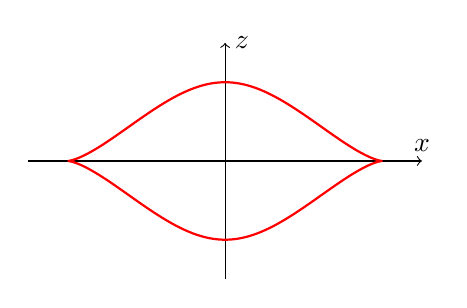
\begin{tikzpicture}[baseline=-.5ex, scale=2]
\draw[->] (-1.25,0) -- (1.25,0) node[above] {$x$};
\draw[->] (0,-0.75) -- (0,0.75) node[right] {$z$};
\draw[thick, red] plot[domain=0:2*pi, samples=200] ({cos(\x r)/ (1+ sin(\x r)^2)}, {-2*sin(\x r)^3/(1+sin(\x r)^2)^2});
\end{tikzpicture}
\]

Let $\legendrian\subset J^1\sphere^1$ be a Legendrian link.
Then the image $\iota(\legendrian)$ can be isotoped into a neighborhood of the Legendrian unknot in $\R^3$.
In particular, if $\legendrian$ is a closure of a positive braid $\beta$, then $\iota(\legendrian)$ looks like a satellite link of the Legendrian unknot in $\R^3$.

We consider a Legendrian surface $\widehat\Legendrian \subset J^1(\sphere^1\times \R_{r>0})$ having cylindrical ends so that for some $S_1>S_2$,
\begin{align*}
\widehat\Legendrian \cap J^1(\sphere^1\times\R_{r\ge e^{S_1}}) &\cong \legendrian_1\times\R_{s\ge S_1},&
\widehat\Legendrian \cap J^1(\sphere^1\times\R_{r\le e^{S_2}}) &\cong \legendrian_2\times\R_{s\le S_2}.
\end{align*}
Then the projection $L_{\widehat\Legendrian}=\pi_L(\psi(\widehat\Legendrian))$ of the surface $\widehat\Legendrian$ inside $\sphere^3\times\R_u$ becomes an exact Lagrangian cobordism from $\iota(\legendrian_1)$ to $\iota(\legendrian_2)$.

Similarly, let $\widehat\Legendrian\subset J^1\R^2$ be a Legendrian surface having a cylindrical end. That is, for some $S\in \R$, 
\[
\widehat\Legendrian\cap J^1\R^2_{r\ge e^S}\cong \legendrian \times \R_{s\ge S}.
\]
Then the projection $L_{\widehat\Legendrian}=\pi_L(\widehat\Legendrian)$ in 
$T^*\R^2\cong(\bbC^2, \omega_{\mathsf{st}})$ becomes an exact Lagrangian filling of $\iota(\legendrian)$.
Note that the Lagrangian $\pi_L(\widehat\Legendrian)$ is embedded if and only if the Legendrian surface $\widehat\Legendrian$ has no Reeb chords.

\begin{lemma}\label{lem:legendrian and lagrangian}
Let $\widehat\Legendrian$ and $\widehat\Legendrian'$ be two Legendrian surfaces in $J^1\R^2$ without Reeb chords having the identical cylindrical ends
\[
\widehat\Legendrian\cap J^1\R^2_{r\ge e^S} \cong \legendrian \times \R_{s\ge S}
\cong
\widehat\Legendrian'\cap J^1\R^2_{r\ge e^S}
\]
for some $S\in\R$.
If the exact embedded Lagrangian fillings $L_{\widehat\Legendrian}=\pi_L(\widehat\Legendrian)$ and $L_{\widehat\Legendrian'}=\pi_L(\widehat\Legendrian')$ of $\iota(\legendrian)$ are exact Lagrangian isotopic, then $\widehat\Legendrian, \widehat\Legendrian'$ are Legendrian isotopic.
\end{lemma}

On the other hand, any compact Legendrian surface $\Legendrian\subset J^1\disk^2$ can be extended to $\widehat\Legendrian\subset J^1\R^2$ by attaching the cylindrical end $\boundary\Legendrian\times[1,\infty)$ in a smooth way.
For two compact Legendrian surfaces $\Legendrian, \Legendrian'\subset J^1\disk^2$, if $\widehat\Legendrian$ and $\widehat\Legendrian'$ are Legendrian isotopic if and only if $\Legendrian$ and $\Legendrian'$ are Legendrian isotopic relative to boundary.

\begin{corollary}
Let $\legendrian\subset J^1\sphere^1$ be a Legendrian link and $\Legendrian, \Legendrian'\subset J^1\disk^2$ be two Legendrian surfaces without Reeb chords whose boundaries are $\legendrian$.
Then two exact embedded Lagrangian fillings $\pi_{L}(\Legendrian)$ and $\pi_{L}(\Legendrian')$ are exact Lagrangian isotopic relative to boundary if and only if $\Legendrian$ and $\Legendrian'$ are Legendrian isotopic relative to boundary without making Reeb chords during the isotopy.
\end{corollary}

\begin{remark}
We are interested in exact Lagrangian fillings of Legendrian links up to \emph{exact Lagrangian isotopy} relative to boundary, 
an isotopy through exact Lagrangian fillings which fixes the Legendrian boundary.
This is equivalent to exact Lagrangian fillings up to \emph{Hamiltonian isotopy}, which is an isotopy through Hamiltonian diffeomorphism fixing the boundary. The similar holds for Lagrangian cobordisms.
\end{remark}

We end this section by investigating certain actions on the symplectic manifold $\sphere^3\times \R_u$ and induced actions on $J^1\sphere^1$.
Especially, we are interested in actions on $\sphere^3\times \R_u$ preserving the $\R_u$-coordinate, the symplectization coordinate. So actions on $\sphere^3$ determine the actions on the symplectic manifold $\sphere^3\times \R_u$.

Recall that $\sphere^3$ is the unit sphere in $\bbC^2$, i.e., coordinates $z_1=r_1 e^{i\theta_1}, z_2=r_2 e^{i\theta_2}$ with $r_1^2 + r_2^2=1$.

\paragraph{Rotation} A symplectomorphism $R_{\theta_0} \colon \sphere^3\times \R_u \to \sphere^3\times \R_u$, called {\em rotation}, is defined by
\[
R_{\theta_0}(z_1, z_2,u)=(z_1\cos\theta_0 -z_2\sin\theta_0, z_1\sin\theta_0+z_2\cos\theta_0,u).
\]
Note that the restriction $R_{\theta_0}|_{\sphere^3}$ fixes the contact form $\alpha_{\sphere^3}$.
Under the symplectic embedding $\Psi:J^1\sphere^1\times \R_s \hookrightarrow \sphere^3\times \R_u$, we have the following induced symplectomorphism
\[
J^1\sphere^1\times \R_s \to J^1\sphere^1\times \R_s,\quad (\theta,p_{\theta},z,s)\mapsto (\theta+\theta_0,p_{\theta},z,s).
\]
By restricting $R_{\theta_0}$ on $J^1\sphere^1$, we obtain
\[
J^1\sphere^1 \to J^1\sphere^1, \quad (\theta,p_{\theta},z)\mapsto (\theta+\theta_0,p_{\theta},z).
\]
%With a slight abuse of notation, let us denote the above three maps by $R_{\theta_0}$.
We are especially interested in $\theta_0=\pi,2\pi/3$. They produce $\Z/2\Z$- and $\Z/3\Z$-action on the symplectic manifold $\sphere^3\times \R_u$ and Lagrangian fillings of satellite links of the Legendrian unknot, respectively.

\paragraph{Conjugation} An anti-symplectic involution $\tau \colon \sphere^3\times\R_u \to \sphere^3\times\R_u$, which we call {\em conjugation},  is defined by
\[
(z_1,z_2,u)\mapsto (\bar z_1,\bar z_2 ,u).
\]
It is direct to check that $\tau$ reverses the sign of symplectic form $\frac{i}{2}(dz_1\wedge d\bar z_1+dz_2\wedge d\bar z_2)$, and its restriction on $\sphere^3$ also reverse the sign of $\alpha_{\sphere^3}$. 
Again by the symplectic embedding~$\Psi$, the conjugation induces an action on $J^1\sphere^1\times \R_s$
\[
(\theta,p_\theta,z,s)\mapsto (\theta,-p_\theta,-z,s)
\]
whose restriction on $J^1\sphere^1$ becomes
\[
(\theta,p_\theta,z)\mapsto (\theta,-p_\theta,-z).
\]
This anti-symplectic involution naturally produce $\Z/2\Z$-action on the symplectic manifold and Lagrangian fillings as in the actions from the rotations.

\begin{figure}[ht]
\subfigure[Rotation\label{figure:rotation unknot}]{
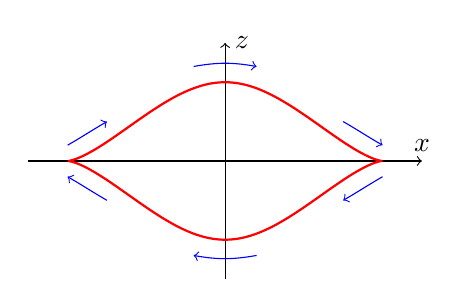
\begin{tikzpicture}[baseline=-.5ex, scale=2]
\draw[->] (-1.25,0) -- (1.25,0) node[above] {$x$};
\draw[->] (0,-0.75) -- (0,0.75) node[right] {$z$};
\draw[thick, red] plot[domain=0:2*pi, samples=200] ({cos(\x r)/ (1+ sin(\x r)^2)}, {-2*sin(\x r)^3/(1+sin(\x r)^2)^2});
\draw[->,blue] (1,-0.1) to[out=210,in=30] (0.75,-0.25);
\draw[->,blue] (0.2,-0.6) to[out=190,in=-10] (-0.2,-0.6);
\draw[->,blue] (-0.75,-0.25) to[out=150,in=-30] (-1,-0.1);
\begin{scope}[rotate=180]
\draw[->,blue] (1,-0.1) to[out=210,in=30] (0.75,-0.25);
\draw[->,blue] (0.2,-0.6) to[out=190,in=-10] (-0.2,-0.6);
\draw[->,blue] (-0.75,-0.25) to[out=150,in=-30] (-1,-0.1);
\end{scope}
\end{tikzpicture}
}
\subfigure[Conjugation\label{figure:conjugation unknot}]{
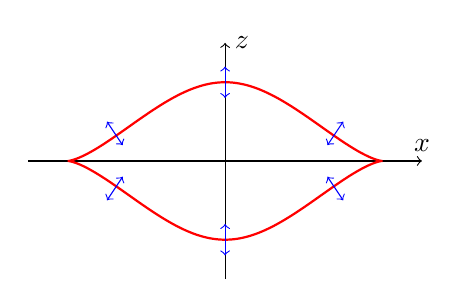
\begin{tikzpicture}[baseline=-.5ex, scale=2]
\draw[->] (-1.25,0) -- (1.25,0) node[above] {$x$};
\draw[->] (0,-0.75) -- (0,0.75) node[right] {$z$};
\draw[thick, red] plot[domain=0:2*pi, samples=200] ({cos(\x r)/ (1+ sin(\x r)^2)}, {-2*sin(\x r)^3/(1+sin(\x r)^2)^2});
\draw[<->,blue] (0.65,-0.1) -- (0.75,-0.25);
\draw[<->,blue] (0,-0.4) -- (0,-0.6);
\draw[<->,blue] (-0.65,-0.1) -- (-0.75,-0.25);
\begin{scope}[rotate=180]
\draw[<->,blue] (0.65,-0.1) -- (0.75,-0.25);
\draw[<->,blue] (0,-0.4) -- (0,-0.6);
\draw[<->,blue] (-0.65,-0.1) -- (-0.75,-0.25);
\end{scope}
\end{tikzpicture}
}
\caption{Rotations and conjugation near the Legendrian unknot.}
\label{fig:actions on the unknot}
\end{figure}

\begin{lemma}\label{lem:rotation and conjugation}
Let $R_{\theta_0}$ and $\eta$ be rotation and conjugation defined on $\sphere^3\times \R$ as above, respectively.  Then the induced maps on the front projection $\pi_{F}:J^1\sphere^1\to\sphere^1\times\R$ becomes as follows:
\begin{align*}
R_{\theta_0}|_{\sphere^1\times \R}&:(\theta,z)\mapsto (\theta+\theta_0,z);\\
\eta|_{\sphere^1\times \R}&:(\theta,z)\mapsto (\theta,-z).
\end{align*}
\end{lemma}



\subsubsection{$N$-graphs on $\disk^2$ and $\annulus$}\label{section:annular Ngraphs}
Let $\beta\subset J^1\R^1$ be a positive $N$-braid given by a word consisting of the generators $\sigma_1,\dots, \sigma_{N-1}$, and let $\legendrian=\legendrian_\beta\in J^1\sphere^1$ be a Legendrian link obtained by the closure of $\beta$, which can be regarded as a satellite of the Legendrian unknot in $\R^3$.
The front projection $\pi_F(\legendrian)\subset \sphere^1\times \R$ of $\legendrian$ consists of $N$-strands with double points corresponding to the braid word $\beta$.
Hence, the Legendrian $\legendrian$ gives us an $(N-1)$-tuple $(\legendrian_1, \legendrian_2,\dots, \legendrian_{N-1})$ of subsets of points in $\sphere^1$, each of which corresponds to the generator $\sigma_i$ in the braid word $\beta$.

Conversely, let $(\legendrian_1,\dots, \legendrian_{N-1})$ be an $(N-1)$-tuple of disjoint\footnote{This condition can be weakened as follows: $\legendrian_i\cap \legendrian_{i+1}=\varnothing$ for each $1\le i<N$.} subsets of $\sphere^1$.
Then, from this data $(\legendrian_1,\dots,\legendrian_{N-1})$, one can build the Legendrian link $\legendrian$, which is the branched $N$-fold covering space of $\sphere^1$ such that the $i$-th and $(i+1)$-st covers are branched along the set $\legendrian_i$.

Let $\ngraph=(\ngraph_1,\dots,\ngraph_{N-1})$ be an $N$-graph on $\disk^2$.
The \emph{boundary} $\boundary\ngraph$ of $\ngraph$ is a Legendrian link defined by an $N$-graph on $\sphere^1=\boundary\disk^2$ as
\[
\boundary\ngraph=(\boundary\ngraph_1,\dots,\boundary\ngraph_{N-1}),\quad
\boundary\ngraph_i\colonequals \ngraph_i\cap \sphere^1\subset \sphere^1.
\]
We say that $\ngraph$ is \emph{of type} $\legendrian$ or $\legendrian$ \emph{admits} an $N$-graph $\ngraph$ if $\boundary\ngraph=\legendrian$.

Let $\annulus$ be the oriented annulus with two boundary components $\boundary_+\annulus$ and $\boundary_-\annulus$.
For an $N$-graph~$\ngraph$ on $\annulus$, let $\boundary_\pm\ngraph\colonequals\ngraph\cap\boundary_\pm\annulus$ be Legendrian links at two boundaries $\boundary_\pm\annulus$, respectively.
We say that $\ngraph$ is \emph{of type} $(\legendrian_+, \legendrian_-)$ if $\boundary_\pm\ngraph=\legendrian_\pm$, respectively.

A typical example of annular $N$-graphs comes from Lagrangian cobordism between Legendrian links, which are closures of positive braids.
In particular, for two closures $\legendrian_1$ and $\legendrian_2$ of positive braids $\beta_1$ and $\beta_2$, any sequence of Legendrian braid moves from $\legendrian_2$ to $\legendrian_1$ will give us a special annular $N$-graph $\ngraph_{\legendrian_2\legendrian_1}$.\footnote{One may call the $N$-graph $\ngraph_{\legendrian_2\legendrian_1}$ a \emph{strict concordance} since it is a union of cylinders.}
Hence, for an $N$-graphs $\ngraph$ with $\boundary\ngraph=\legendrian_1$, we have the $N$-graph $\ngraph_{\legendrian_2\legendrian_1}\ngraph$ with boundary
\[
\boundary(\ngraph_{\legendrian_2\legendrian_1}\ngraph)=\legendrian_2.
\]

\begin{remark}
We are dealing with both Legendrian links $\legendrian$ and surfaces $\Legendrian$.
In order to avoid the confusion, we use the terminologies ``$\boundary$-Legendrian isotopy'' and ``Legendrian isotopy'' for isotopies between Legendrian links and surfaces, respectively.
\end{remark}

Since a closure of a Legendrian positive braid in $J^1\sphere^1$ should not have any cusp, possible $\boundary$-Legendrian isotopies are either plane isotopies \Move{R0} or the third Reidemeister move \Move{RIII} as follows:
\begin{center}
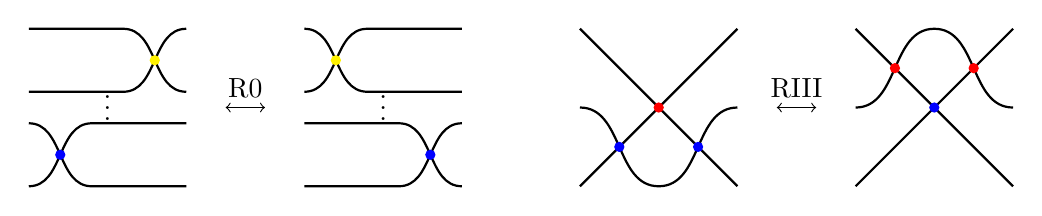
\begin{tikzpicture}
\begin{scope}
\draw[thick] (1,1) to[out=180,in=0] (0.2,0.2) to (-1,0.2);
\draw[thick] (1,0.2) to[out=180,in=0] (0.2,1) to (-1,1);

\node at (0,0.1) {$\vdots$};

\draw[thick] (1,-0.2) to (-0.2,-0.2) to[out=180,in=0] (-1,-1);
\draw[thick] (1,-1) to (-0.2,-1) to[out=180,in=0] (-1,-0.2);

\draw[thick,yellow,fill=yellow] (0.6,0.6) circle (0.05);
\draw[thick,blue,fill=blue] (-0.6,-0.6) circle (0.05);

\draw [<->] (1.5,0) -- (2,0) node[midway, above] {\Move{R0}};
\end{scope}


\begin{scope}[xshift=3.5cm]
\draw[thick] (-1,1) to[out=0,in=180] (-0.2,0.2) to (1,0.2);
\draw[thick] (-1,0.2) to[out=0,in=180] (-0.2,1) to (1,1);

\node at (0,0.1) {$\vdots$};

\draw[thick] (-1,-0.2) to (0.2,-0.2) to[out=0,in=180] (1,-1);
\draw[thick] (-1,-1) to (0.2,-1) to[out=0,in=180] (1,-0.2);

\draw[thick,yellow,fill=yellow] (-0.6,0.6) circle (0.05);
\draw[thick,blue,fill=blue] (0.6,-0.6) circle (0.05);
\end{scope}

\begin{scope}[xshift=7cm]
\draw[thick] (-1,-1) to (1,1);
\draw[thick] (-1,1) to (1,-1);
\draw[thick] (-1,0) to[out=0, in=180] (0,-1) to[out=0,in=180] (1,0);

\draw[thick,blue,fill=blue] (-0.5,-0.5) circle (0.05);
\draw[thick,blue,fill=blue] (0.5,-0.5) circle (0.05);
\draw[thick,red,fill=red] (0,0) circle (0.05);

\draw [<->] (1.5,0) -- (2,0) node[midway, above] {\Move{RIII}};
\end{scope}

\begin{scope}[xshift=10.5cm]
\draw[thick] (-1,-1) to (1,1);
\draw[thick] (-1,1) to (1,-1);
\draw[thick] (-1,0) to[out=0, in=180] (0,1) to[out=0,in=180] (1,0);

\draw[thick,red,fill=red] (-0.5,0.5) circle (0.05);
\draw[thick,red,fill=red] (0.5,0.5) circle (0.05);
\draw[thick,blue,fill=blue] (0,0) circle (0.05);

\end{scope}
\end{tikzpicture}
\end{center}

Therefore, any annular $N$-graph corresponding to a sequence of Reidemeister moves between Legendrian links is a concatenation of \emph{elementary annular $N$-graphs}, which are  $\ngraph_{\Move{R0}}$ and $\ngraph_{\Move{RIII}}$ on the annulus $\annulus$ as depicted in Figure~\ref{fig:elementary annulus N-graph}.
We call an annular $N$-graph \emph{tame} if it is a concatenation of elementary annular $N$-graphs. 

\begin{figure}[ht]
\subfigure[Annular $N$-graph \Move{R0}]{\makebox[0.45\textwidth]{$
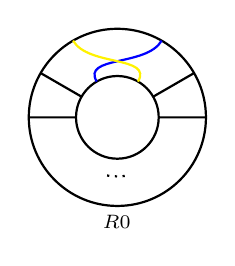
\begin{tikzpicture}[baseline=-.5ex,scale=0.75]
\draw [thick] (0,0) circle [radius=0.7];
\draw [thick] (0,0) circle [radius=1.5];
\draw [thick, dotted] (260:1) arc (260:280:1);
\draw [thick, blue] (120:0.7) to[out=120, in=-120] (60:1.5);
\draw [thick, yellow] (60:0.7) to[out=60,in=-60] (120:1.5);
\draw [thick, black]
(30:0.7) -- (30:1.5) 
(150:0.7) -- (150:1.5)
(0:0.7) -- (0:1.5) 
(180:0.7) -- (180:1.5);
\node[below] at (0,-1.5) {$\ngraph_{\Move{R0}}$};
\end{tikzpicture}
\cdot
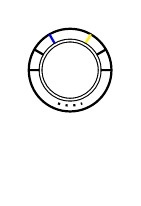
\begin{tikzpicture}[baseline=-.5ex,scale=0.75]
\draw [thick] (0,0) circle [radius=0.7];
\draw [thick, black]
(30:0.5) -- (30:0.7) 
(150:0.5) -- (150:0.7)
(0:0.5) -- (0:0.7) 
(180:0.5) -- (180:0.7);
\draw [thick, yellow] (60:0.5) -- (60:0.7);
\draw [thick, blue] (120:0.5) -- (120:0.7) ;
\draw [thick, dotted] (250:0.6) arc (250:290:0.6);
\draw [double] (0,0) circle [radius=0.5];
\node[below] at (0,-1.5) {$\ngraph$};
\end{tikzpicture}
=
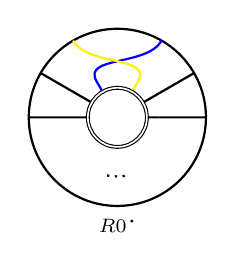
\begin{tikzpicture}[baseline=-.5ex,scale=0.75]
\draw [thick] (0,0) circle [radius=1.5];
\draw [thick, dotted] (260:1) arc (260:280:1);
\draw [thick, blue] (120:0.7) to[out=120, in=-120] (60:1.5);
\draw [thick, yellow] (60:0.7) to[out=60,in=-60] (120:1.5);
\draw [thick, black]
(30:0.7) -- (30:1.5) 
(150:0.7) -- (150:1.5)
(0:0.7) -- (0:1.5) 
(180:0.7) -- (180:1.5);
\draw [thick, black]
(30:0.5) -- (30:0.7) 
(150:0.5) -- (150:0.7)
(0:0.5) -- (0:0.7) 
(180:0.5) -- (180:0.7);
\draw [thick, yellow] (60:0.5) -- (60:0.7);
\draw [thick, blue] (120:0.5) -- (120:0.7) ;
\draw [double] (0,0) circle [radius=0.5];
\node[below] at (0,-1.5) {$\ngraph_{\Move{R0}}\cdot\ngraph$};
\end{tikzpicture}$
}}
\subfigure[Annular $N$-graph \Move{RIII}]{\makebox[0.45\textwidth]{$
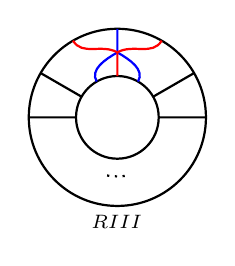
\begin{tikzpicture}[baseline=-.5ex,scale=0.75]
\draw [thick] (0,0) circle [radius=0.7];
\draw [thick] (0,0) circle [radius=1.5];
\draw [thick, dotted] (260:1) arc (260:280:1);
\draw [thick, blue] (60:0.7) to[out=60, in=-30] (90:1.1) (120:0.7) to[out=120, in=-150] (90:1.1) -- (90:1.5);
\draw [thick, red] (90:0.7) -- (90:1.1) to[out=150,in=-60] (120:1.5) (90:1.1) to[out=30,in=-120] (60:1.5);
\draw [thick, black]
(30:0.7) -- (30:1.5) 
(150:0.7) -- (150:1.5)
(0:0.7) -- (0:1.5) 
(180:0.7) -- (180:1.5);
\node[below] at (0,-1.5) {$\ngraph_{\Move{RIII}}$};
\end{tikzpicture}
\cdot
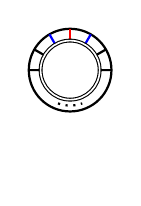
\begin{tikzpicture}[baseline=-.5ex,scale=0.75]
\draw [thick] (0,0) circle [radius=0.7];
\draw [thick, black]
(30:0.5) -- (30:0.7) 
(150:0.5) -- (150:0.7)
(0:0.5) -- (0:0.7) 
(180:0.5) -- (180:0.7);
\draw [thick, red] (90:0.5) -- (90:0.7);
\draw [thick, blue] (60:0.5) -- (60:0.7) (120:0.5) -- (120:0.7) ;
\draw [thick, dotted] (250:0.6) arc (250:290:0.6);
\draw [double] (0,0) circle [radius=0.5];
\node[below] at (0,-1.5) {$\ngraph$};
\end{tikzpicture}
=
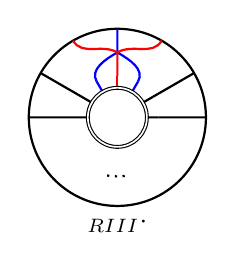
\begin{tikzpicture}[baseline=-.5ex,scale=0.75]
\draw [thick] (0,0) circle [radius=1.5];
\draw [thick, dotted] (260:1) arc (260:280:1);
\draw [thick, blue] (60:0.7) to[out=60, in=-30] (90:1.1) (120:0.7) to[out=120, in=-150] (90:1.1) -- (90:1.5);
\draw [thick, red] (90:0.7) -- (90:1.1) to[out=150,in=-60] (120:1.5) (90:1.1) to[out=30,in=-120] (60:1.5);
\draw [thick, black]
(30:0.7) -- (30:1.5) 
(150:0.7) -- (150:1.5)
(0:0.7) -- (0:1.5) 
(180:0.7) -- (180:1.5);
\draw [thick, black]
(30:0.5) -- (30:0.7) 
(150:0.5) -- (150:0.7)
(0:0.5) -- (0:0.7) 
(180:0.5) -- (180:0.7);
\draw [thick, red] (90:0.5) -- (90:0.7);
\draw [thick, blue] (60:0.5) -- (60:0.7) (120:0.5) -- (120:0.7) ;
\draw [double] (0,0) circle [radius=0.5];
\node[below] at (0,-1.5) {$\ngraph_{\Move{RIII}}\cdot\ngraph$};
\end{tikzpicture}$
}}
\caption{$\boundary$-Legendrian isotopy and elementary annulus $N$-graphs}
\label{fig:elementary annulus N-graph}
\end{figure}

\begin{example}
A \emph{rotational annular $N$-graph}, which has no vertices and rotates a certain angle as depicted below is tame.
\[
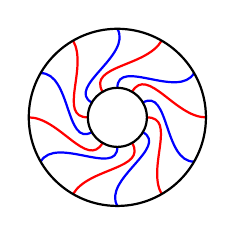
\begin{tikzpicture}[baseline=-.5ex, scale=0.75]
\draw [thick, red] (0.5*1/2,{1/2*sqrt(3)/2}) to[out=60,in=180] (1.5,0);
\draw [rotate around={60:(0,0)},thick, red] (0.5*1/2,{1/2*sqrt(3)/2}) to[out=60,in=180] (1.5,0);
\draw [rotate around={120:(0,0)},thick, red] (0.5*1/2,{1/2*sqrt(3)/2}) to[out=60,in=180] (1.5,0);
\draw [rotate around={180:(0,0)},thick, red] (0.5*1/2,{1/2*sqrt(3)/2}) to[out=60,in=180] (1.5,0);
\draw [rotate around={240:(0,0)},thick, red] (0.5*1/2,{1/2*sqrt(3)/2}) to[out=60,in=180] (1.5,0);
\draw [rotate around={300:(0,0)},thick, red] (0.5*1/2,{1/2*sqrt(3)/2}) to[out=60,in=180] (1.5,0);

\draw [thick, blue] ({1.5*sqrt(3)/2},{1.5*1/2}) to[out=-120, in=90] (0,0.5);
\draw [rotate around={60:(0,0)}, thick, blue] ({1.5*sqrt(3)/2},{1.5*1/2}) to[out=-120, in=90] (0,0.5);
\draw [rotate around={120:(0,0)}, thick, blue] ({1.5*sqrt(3)/2},{1.5*1/2}) to[out=-120, in=90] (0,0.5);
\draw [rotate around={180:(0,0)}, thick, blue] ({1.5*sqrt(3)/2},{1.5*1/2}) to[out=-120, in=90] (0,0.5);
\draw [rotate around={240:(0,0)}, thick, blue] ({1.5*sqrt(3)/2},{1.5*1/2}) to[out=-120, in=90] (0,0.5);
\draw [rotate around={300:(0,0)}, thick, blue] ({1.5*sqrt(3)/2},{1.5*1/2}) to[out=-120, in=90] (0,0.5);

\draw [thick] (0,0) circle [radius=1.5];
\draw [thick] (0,0) circle [radius=0.5];
\end{tikzpicture}
\]

It is known that the rotational annular $N$-graph acts on the set of $N$-graphs for the Legendrian torus link $\legendrian(n,m)$ of maximal Thurston--Bennequin number.
This type of annular $N$-graphs play a crucial role in producing a sequence of distinct exact Lagrangian fillings of positive braid Legendrian links, see \cite{Kal2006, CG2020, GSW2020b}.
\end{example}


\begin{definition}\label{def:boundary Legendrian isotopic}
We say that two $N$-graphs $\ngraph$ and $\ngraph'$ with $\boundary\ngraph=\legendrian_1$ and $\boundary\ngraph=\legendrian_2$ are \emph{$\boundary$-Legendrian isotopic} if there exists a tame annular $N$-graph $\ngraph_{\legendrian_2\legendrian_1}$ such that $[\ngraph']= [\ngraph_{\legendrian_2\legendrian_1}\ngraph]$.
\end{definition}




\subsubsection{Stabilizations}
For a positive $N$-braid $\beta$ in $J^1\R^1$, a \emph{stabilization} $S(\beta)$ is a positive $(N+1)$-braid which satisfies the following:
\begin{enumerate}
\item Closures of $\beta$ and $S(\beta)$ are Legendrian isotopic in $\sphere^3$:
\[
\legendrian_\beta \cong \legendrian_{S(\beta)}.
\]
\item The braid $\beta$ can be recovered by forgetting a strand from $S(\beta)$.
\end{enumerate}
More precisely, the second condition is as follows:
let $q_{i+}(\beta)$ and $q_{i-}(\beta)$ be braids obtained from~$\beta$ by forgetting the $i$-th strand from the left and from the right.
Then $S(\beta)$ has a decomposition
\[
S(\beta)=\beta_1\sigma_j\beta_2
\]
and there exists an index $1\le i\le N+1$ such that the $i$-th strands from the left and from the right of $\beta$ meet precisely at the crossing $\sigma_j$ in the middle of the decomposition $\beta=\beta_1\sigma_j\beta_2$ and moreover
\[
\beta= q_{i+}(\beta_1) q_{i-}(\beta_2).
\]

The most typical example of a stabilization is as follows:
let $\beta_0$ be a positive $N$-braid and $\beta=\Delta_N\beta_0\Delta_N$, where $\Delta_N$ is the half-twist $N$-braid.
Then it determines a Legendrian link $\legendrian_\beta$ uniquely up to Legendrian isotopy, but the converse is not true.
Indeed, there are infinitely many pairwise distinct positive braids whose rainbow closures are Legendrian isotopic to $\legendrian_\beta$ in $\sphere^3$.
In particular, for a positive $N$-braid $\beta_0$, a \emph{stabilization} $S(\beta_0)$ is a positive $(N+1)$-braid defined by
$S(\beta_0) = \beta_0\sigma_N$, where $\beta_0$ in $S(\beta_0)$ is regarded as an $(N+1)$-braid by adding a trivial $(N+1)$-st strand.
Let $S(\beta) = \Delta_{N+1}S(\beta_0)\Delta_{N+1}$. Then 
\begin{align*}
S(\beta) &= \Delta_{N+1} (\beta_0 \sigma_N) \Delta_{N+1}
=(\sigma_1\dots\sigma_N) (\Delta_N \beta_0 \Delta_N) (\sigma_N\dots\sigma_1) \sigma_1
\mathrel{\dot{=}} \beta (\sigma_N\dots\sigma_2\sigma_1^3\sigma_2\dots\sigma_N),
\end{align*}
where $\mathrel{\dot{=}}$ means the same up to cyclic permutation of braid words.

\begin{figure}[ht]
\[
\setlength\arraycolsep{2pt}
\begin{array}{rcccc}
\legendrian_\beta&=&
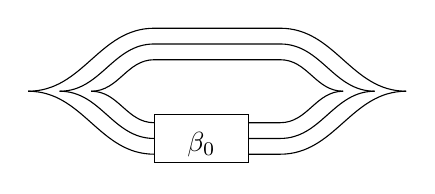
\begin{tikzpicture}[baseline=-.5ex,scale=0.8]
\draw (-1,-1.125) rectangle node[yshift=-.5ex] {$\beta_0$} (0.5,-0.375);
%
\draw (-3,0) to[out=0,in=180] (-1,1) -- (1,1) to[out=0,in=180] (3,0);
\draw (-3,0) to[out=0,in=180] (-1,-1) (0.5,-1) -- (1,-1) to[out=0,in=180] (3,0);
%
\draw (-2.5,0) to[out=0,in=180] (-1,0.75) -- (1,0.75) to[out=0,in=180] (2.5,0);
\draw (-2.5,0) to[out=0,in=180] (-1,-0.75) (0.5,-0.75) -- (1,-0.75) to[out=0,in=180] (2.5,0);
%
\draw (-2,0) to[out=0,in=180] (-1,0.5) -- (1,0.5) to[out=0,in=180] (2,0);
\draw (-2,0) to[out=0,in=180] (-1,-0.5) (0.5,-0.5) -- (1,-0.5) to[out=0,in=180] (2,0);
\end{tikzpicture}
&=&
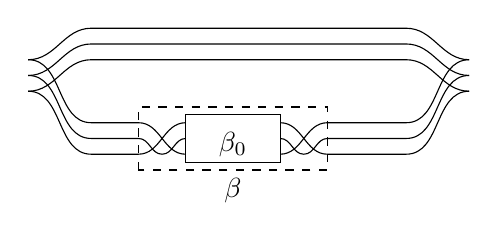
\begin{tikzpicture}[baseline=-.5ex,scale=0.8]
%
\draw[fill=white] (-1,-1.125) rectangle node[yshift=-.5ex] {$\beta_0$} (0.5,-0.375);
%
\draw (-3.5,0.5) to[out=0,in=180] (-2.5, 1) -- (2.5,1) to[out=0,in=180] (3.5,0.5);
\draw (-3.5,0.5) to[out=0,in=180] (-2.5,-0.5) -- (-1.75,-0.5) to[out=0,in=180] (-1, -1)
(0.5,-1) to[out=0,in=180] (1.25, -0.5) to[out=0,in=180] (2,-0.5) -- (2.5,-0.5) to[out=0,in=180] (3.5,0.5);
%
\draw (-3.5,0.25) to[out=0,in=180] (-2.5, 0.75) -- (2.5,0.75) to[out=0,in=180] (3.5,0.25);
\draw (-3.5,0.25) to[out=0,in=180] (-2.5,-0.75) -- (-1.75,-0.75) to[out=0,in=180] (-1.375,-1) to[out=0,in=180] (-1, -0.75)
(0.5,-0.75) to[out=0,in=180] (0.875, -1) to[out=0,in=180] (1.25,-0.75) -- (2.5,-0.75) to[out=0,in=180] (3.5,0.25);
%
\draw (-3.5,0) to[out=0,in=180] (-2.5, 0.5) -- (2.5,0.5) to[out=0,in=180] (3.5,0);
\draw (-3.5,0) to[out=0,in=180] (-2.5,-1) -- (-1.75,-1) to[out=0,in=180] (-1,-0.5)
(0.5,-0.5) to[out=0,in=180] (1.25, -1) -- (2.5,-1) to[out=0,in=180] (3.5,0);
%
\draw[dashed] (-1.75, -1.25) rectangle node[below=2.5ex] {$\beta$} (1.25, -0.25);
\end{tikzpicture}
\\
\legendrian_{S(\beta)}&=&
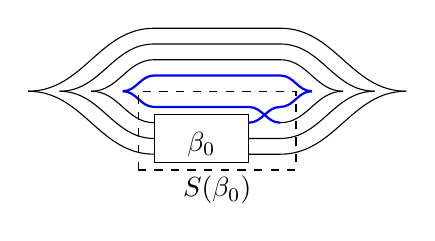
\begin{tikzpicture}[baseline=-.5ex,scale=0.8]
\draw (-1,-1.125) rectangle node[yshift=-.5ex] {$\beta_0$} (0.5,-0.375);
%
\draw (-3,0) to[out=0,in=180] (-1,1) -- (1,1) to[out=0,in=180] (3,0);
\draw (-3,0) to[out=0,in=180] (-1,-1) (0.5,-1) -- (1,-1) to[out=0,in=180] (3,0);
%
\draw (-2.5,0) to[out=0,in=180] (-1,0.75) -- (1,0.75) to[out=0,in=180] (2.5,0);
\draw (-2.5,0) to[out=0,in=180] (-1,-0.75) (0.5,-0.75) -- (1,-0.75) to[out=0,in=180] (2.5,0);
%
\draw (-2,0) to[out=0,in=180] (-1,0.5) -- (1,0.5) to[out=0,in=180] (2,0);
\draw (-2,0) to[out=0,in=180] (-1,-0.5) (1,-0.5) to[out=0,in=180] (2,0);
%
\draw[thick,blue] (-1.5,0) to[out=0,in=180] (-1,0.25) -- (1,0.25) to[out=0,in=180] (1.5,0);
\draw[thick,blue] (-1.5,0) to[out=0,in=180] (-1,-0.25) (1,-0.25) to[out=0,in=180] (1.5,0);
\draw[thick,blue] (-1,-0.25) -- (0.5,-0.25) to[out=0,in=180] (1,-0.5) (0.5,-0.5) to[out=0,in=180] (1,-0.25);
%
\draw[dashed] (-1.25,-1.25) rectangle node[below=3ex] {$S(\beta_0)$} (1.25, 0);
\end{tikzpicture}
&=&
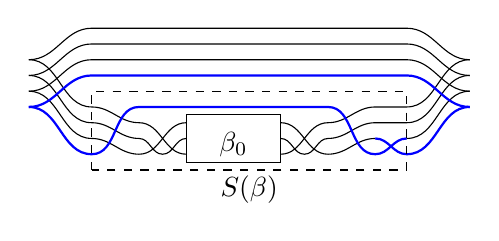
\begin{tikzpicture}[baseline=-.5ex,scale=0.8]
%
\draw[fill=white] (-1,-1.125) rectangle node[yshift=-.5ex] {$\beta_0$} (0.5,-0.375);
%
\draw (-3.5,0.5) to[out=0,in=180] (-2.5, 1) -- (2.5,1) to[out=0,in=180] (3.5,0.5);
\draw (-3.5,0.5) to[out=0,in=180] (-2.5,-0.25) to[out=0,in=180] (-1.75, -0.5) to[out=0,in=180] (-1,-1)
(0.5,-1) to[out=0,in=180] (1.25,-0.5) to[out=0,in=180] (2,-0.25) to[out=0,in=180] (2.5,-0.25) to[out=0,in=180] (3.5,0.5);
%
\draw (-3.5,0.25) to[out=0,in=180] (-2.5, 0.75) -- (2.5,0.75) to[out=0,in=180] (3.5,0.25);
\draw (-3.5,0.25) to[out=0,in=180] (-2.5,-0.5) to[out=0,in=180] (-1.75,-0.75) to[out=0,in=180] (-1.375, -1) to[out=0,in=180] (-1, -0.75)
(0.5,-0.75) to[out=0,in=180] (0.875, -1) to[out=0,in=180] (1.25, -0.75) to[out=0,in=180] (2,-0.5) -- (2.5,-0.5) to[out=0,in=180] (3.5,0.25);
%
\draw (-3.5,0) to[out=0,in=180] (-2.5, 0.5) -- (2.5,0.5) to[out=0,in=180] (3.5,0);
\draw (-3.5,0) to[out=0,in=180] (-2.5,-0.75) to[out=0,in=180] (-1.75,-1) to[out=0,in=180] (-1,-0.5)
(0.5, -0.5) to[out=0,in=180] (1.25, -1) to[out=0,in=180] (2,-0.75) (2.5,-0.75) to[out=0,in=180] (3.5,0);
%
\draw[thick,blue] (-3.5,-0.25) to[out=0,in=180] (-2.5, 0.25) -- (2.5,0.25) to[out=0,in=180] (3.5,-0.25);
\draw[thick,blue] (-3.5,-0.25) to[out=0,in=180] (-2.5, -1) to[out=0,in=180] (-1.75, -0.25) -- (1.25, -0.25) to[out=0,in=180] (2,-1) to[out=0,in=180] (2.5,-0.75) (2,-0.75) to[out=0,in=180] (2.5,-1) to[out=0,in=180] (3.5,-0.25);
%
\draw[dashed] (-2.5,-1.25) rectangle node[below=3ex] {$S(\beta)$} (2.5,0);
\end{tikzpicture}
\end{array}
\]
\caption{A stabilization $\legendrian_{S(\beta)}$ of a Legendrian link $\legendrian_\beta$}
\label{figure:stabilization of Legendrian}
\end{figure}

The Legendrian $\legendrian_{S(\beta)}$ does depend on the braid word $\beta_0$.
For example, for each pair of positive $N$-braids $\beta_0^{(1)}$ and $\beta_0^{(2)}$ with $\beta_0=\beta_0^{(1)}\beta_0^{(2)}$, let $\beta_0'=\beta_0^{(2)}\beta_0^{(1)}$ and $\beta' = \Delta_N\beta_0'\Delta_N$.
Then two Legendrian links $\legendrian_\beta$ and $\legendrian_{\beta'}$ are Legendrian isotopic but $\legendrian_{S(\beta)}$ and $\legendrian_{S(\beta')}$ are \emph{not} Legendrian isotopic in general.
Therefore a stabilization of a Legendrian link $\legendrian$ which is a closure of a positive braid may not be uniquely determined.

\begin{example}\label{example:stabilization of An}
Let $\beta(a,b,c)=\sigma_2\sigma_1^{a+1}\sigma_2\sigma_1^{b+1}\sigma_2\sigma_1^{c+1}$ and $\beta(n)=\sigma_1^{n+3}$.
Since $\beta(\dynA_n)=\sigma_1^{n+3} = \sigma_1^{c}\sigma_1^{b+2}$, we have
\begin{align*}
S(\beta(\dynA_n))&=(\sigma_1\sigma_2)\sigma_1^{c}\sigma_1^{b+2}(\sigma_2\sigma_1)\sigma_1\mathrel{\dot{=}}\sigma_1^{b+2} (\sigma_2\sigma_1^3\sigma_2) \sigma_1^{c}
=\sigma_1^{b+1}\Delta_3 \sigma_1 \Delta_3 \sigma_1^{c-1}\\
&=\sigma_1^{b+1} \sigma_2\Delta_3^2\sigma_1^{c-1}
=\sigma_1^{b+1}\sigma_2\sigma_1^{c+1}\sigma_2\sigma_1^2\sigma_2
\mathrel{\dot{=}}\beta(1,b,c).
\end{align*}
Therefore $\beta(1,b,c)$ is a stabilization of $\beta(n)$ for each $b+c-1=n$.
\end{example}

Let us define 
\[
\tilde\beta_0(a,b,c)=
(\sigma_2\sigma_{1,3}\sigma_2) \sigma_2^{a-1}\sigma_1^{b-1}\sigma_3^{c-1}\quad\text{ and }\quad
\tilde\beta(a,b,c)=
(\sigma_2\sigma_{1,3}\sigma_2)^3 \sigma_2^{a-1} \sigma_1^{b+1}\sigma_3^{c+1},
\]
where $\sigma_{1,3}$ is a $4$-braid isotopic to $\sigma_1\sigma_3$ (or equivalently, $\sigma_3\sigma_1$) such that two crossings $\sigma_1$ and $\sigma_3$ occur simultaneously.
Then one can easily show that $\tilde\beta(a,b,c)$ is Legendrian isotopic to $\Delta_4\tilde\beta_0(a,b,c)\Delta_4$.

\begin{example}
The Legendrian $\legendrian_{\tilde\beta_0(a,b,c)}$ is a stabilization of $\legendrian_{\beta_0(a,b,c)}$ since 
\begin{align*}
S(\beta_0(a,b,c)) &= \sigma_1\sigma_2^a \sigma_1^{b-1} \sigma_2 {\color{blue}\sigma_3}\sigma_2^{c-1}
=\sigma_1\sigma_2^a \sigma_1^{b-1}\sigma_3^{c-1} \sigma_2\sigma_3
\mathrel{\dot{=}}(\sigma_2 \sigma_{1,3} \sigma_2) \sigma_2^{a-1} \sigma_1^{b-1}\sigma_3^{c-1}
=\tilde\beta(a,b,c).
\end{align*}
\end{example}

In particular, for $b=c$, we have $4$-braids
\[
\tilde\beta_0(a,b,b)=
(\sigma_2\sigma_{1,3}\sigma_2) \sigma_2^{a-1}\sigma_{1,3}^{b-1}\quad\text{ and }\quad
\tilde\beta(a,b,b)=
(\sigma_2\sigma_{1,3}\sigma_2)^3 \sigma_2^{a-1}\sigma_{1,3}^{b-1},
\]
and denote $\tilde\beta(2,2,n-1)$ and $\tilde\beta(2,3,3)$ by $\tilde\beta(\dynD_{n+1})$ and $\tilde\beta(\dynE_6)$, respectively.
Recall the conjugate action on $\mathbb{C}^2$, which turns links upside down so that in terms of braid words, it interchanges $\sigma_i$ and $\sigma_{N-i}$ for each $N$-braid.
Hence, for $4$-braids, it preserves $\sigma_{1,3}$. Therefore $\tilde\beta(a,b,b)$ is invariant under conjugation and so is $\legendrian_{\tilde\beta(a,b,b)}$:
\begin{lemma}
The Legendrian $\legendrian_{\tilde\beta(a,b,b)}$ is invariant under conjugation.
\end{lemma}

\begin{corollary}\label{corollary:invariance under conjugation}
The Legendrians $\legendrian_{\tilde\beta(\dynD_{n+1})}$ and $\legendrian_{\tilde\beta(\dynE_6)}$ are invariant under conjugation.
\end{corollary}


On the other hand, a stabilization $\legendrian_{S(\beta)}$ of $\legendrian_\beta$ will be represented by $N$-colored dots in $S^1$ while $\legendrian_\beta$ uses only $(N-1)$ colors. That is,
\[
\legendrian_{S(\beta)} \longleftrightarrow 
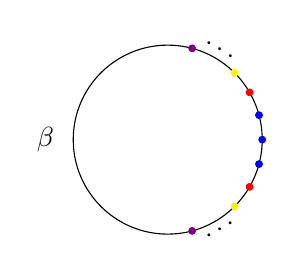
\begin{tikzpicture}[baseline=-.5ex, scale=0.6]
\draw (0,0) circle (2);
\curlybrace[]{90}{270}{2.2};
\draw (180:2.2) node[left] {$\beta$};
\draw[fill, violet] (75:2) circle (2pt) (-75:2) circle (2pt);
\draw[fill, yellow] (45:2) circle (2pt) (-45:2) circle (2pt);
\draw[fill, red] (30:2) circle (2pt) (-30:2) circle (2pt);
\draw[fill, blue] (15:2) circle (2pt) (-15:2) circle (2pt) (0:2) circle (2pt);
\draw (60:2.2) node[rotate=-30] {$\dots$} (-60:2.2) node[rotate=30] {$\dots$};
\end{tikzpicture}\subset J^1\sphere^1
\]
Then one can transfer an $N$-graph $\ngraph$ for $\legendrian_\beta$ into an $(N+1)$-graph $S(\ngraph)$ for $\legendrian_{S(\beta)}$ as follows:
\begin{center}
\begin{tikzcd}
\ngraph=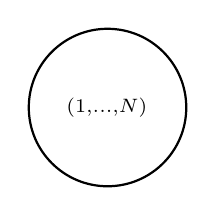
\begin{tikzpicture}[baseline=-.5ex]
\draw [thick] (0,0) circle [radius=1];
\node at (0,0) {$\ngraph_{(1,\dots,N)}$};
\end{tikzpicture}
\arrow[leftrightarrow,"\mathrm{(S)}",r]&
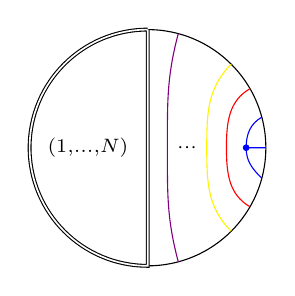
\begin{tikzpicture}[baseline=-.5ex]
\draw (0,0) circle (1.5);
\draw[double] (0,1.5) -- (0,-1.5) arc (-90:-270:1.5);
\draw (-0.75,0) node {$\ngraph_{(1,\dots,N)}$};
\draw[violet] (-75:1.5) to[out=105,in=-90] (0.25,0) to[out=90,in=-105] (75:1.5);
\draw[yellow] (-45:1.5) to[out=135,in=-90] (0.75,0) to[out=90,in=-135] (45:1.5);
\draw[red] (-30:1.5) to[out=150,in=-90] (1,0) to[out=90,in=-150] (30:1.5);
\draw (0.5,0) node {$\scriptstyle\cdots$};
\draw[blue] (-15:1.5) to[out=135,in=-90] (1.25,0) to[out=90,in=-150] (15:1.5) (1.25,0) -- (1.5,0);
\draw[fill,blue] (1.25,0) circle (1pt);
\end{tikzpicture}=S(\ngraph)
\end{tikzcd}
\end{center}




\subsubsection{Annular $N$-graphs and Legendrian loops}
Let $\beta, \beta_+, \beta_-\subset J^1\R^1$ be Legendrian positive $N$-braids.
We denote by $\Ngraphs(\beta)$ and $\Ngraphs(\beta_+, \beta_-)$ the sets of equivalence classes of $N$-graphs on $\disk^2$ and $\annulus$ satisfying boundary conditions given by the closure $\legendrian_\beta$ or a pair of closures $(\legendrian_{\beta_+}, \legendrian_{\beta_-})$.
\begin{align*}
\Ngraphs(\beta)&\colonequals
\{[\ngraph]\mid \ngraph\text{ is an $N$-graph on $\disk^2$ of type $\legendrian_\beta$}\}\\
\Ngraphs(\beta_+, \beta_-)&\colonequals
\{[\ngraph]\mid \ngraph\text{ is an $N$-graph on $\annulus$ of type $(\legendrian_{\beta_+}, \legendrian_{\beta_-})$}\}.
\end{align*}
Here, we are assuming that we are aware of where each braid word starts.

Then it is direct to check that these sets are invariant under the cyclic rotation of the braid words up to bijection. More precisely, for $N$-braids $\beta^{(1)}, \beta^{(2)}$ and $\beta^{(1)}_\pm, \beta^{(2)}_\pm$, closures of $\beta^{(1)}\beta^{(2)}$ and $\beta^{(2)}\beta^{(1)}$ are identical in $J^1\sphere^1$ and there are one-to-one correspondences between sets of $N$-graphs
\begin{align}
\begin{split}
\Ngraphs\left(\beta^{(1)}\beta^{(2)}\right) &\cong \Ngraphs\left(\beta^{(2)}\beta^{(1)}\right),
\end{split}\\
\begin{split}
\Ngraphs\left(\beta_+, \beta^{(1)}_-\beta^{(2)}_-\right) &\cong \Ngraphs\left(\beta_+, \beta^{(2)}_-\beta^{(1)}_-\right),\\
\Ngraphs\left(\beta^{(1)}_+\beta^{(2)}_+, \beta_-\right) &\cong \Ngraphs\left(\beta^{(2)}_+\beta^{(1)}_+, \beta_-\right)
\end{split}
\label{equation:cyclic rotation of word}
\end{align}

Suppose that $\ngraph_1\in\Ngraphs(\beta_2,\beta_1)$ and $\ngraph_2\in\Ngraphs(\beta_3,\beta_2)$.
Then two $N$-graphs can be merged or piled in a natural way to obtain the annular $N$-graph, denoted by~$\ngraph_2\ngraph_1\in\Ngraphs(\beta_3, \beta_1)$.
On the other hand, for $\ngraph\in\Ngraphs(\beta)$ and $\ngraph_1\in\Ngraphs(\beta', \beta)$, the concatenation $\ngraph_1\ngraph\in\Ngraphs(\beta')$ is well-defined by gluing along the boundary $\legendrian_\beta$.
Hence, we have two natural maps
\begin{align*}
\Ngraphs(\beta_3,\beta_2)\times\Ngraphs(\beta_2,\beta_1)&\to \Ngraphs(\beta_3,\beta_1),\\
\Ngraphs(\beta', \beta)\times\Ngraphs(\beta) &\to \Ngraphs(\beta').
\end{align*}

In particular, for each $\boundary$-Legendrian isotopy from $\legendrian'=\legendrian_{\beta'}$ and $\legendrian=\legendrian_\beta$, we have a tame annular $N$-graph $\ngraph_{\legendrian'\legendrian}\in\Ngraphs(\beta',\beta)$, where $\legendrian$ and $\legendrian'$ are closures of $\beta$ and $\beta'$, respectively.
Moreover, we also have a tame annular $N$-graph $\ngraph^{-1}_{\legendrian'\legendrian}$ obtained by flipping the annulus inside out corresponding to the inverse isotopy from $\legendrian$ to $\legendrian'$.
Hence, we have two maps inverses to each other
\[
\Ngraphs(\beta) \to \Ngraphs(\beta'),\quad\text{ and }\quad
\Ngraphs(\beta')\to \Ngraphs(\beta),
\]
defined by
\[
\ngraph\mapsto \ngraph_{\legendrian'\legendrian}\cdot\ngraph,\quad\text{ and }\quad
\ngraph'\mapsto \ngraph^{-1}_{\legendrian'\legendrian}\cdot\ngraph',
\]
respectively.

Let $\Ngraphs_0(\beta,\beta)$ be the subset of tame annular $N$-graphs of type $(\beta,\beta)$.
\begin{lemma}
Let $\beta$ be a Legendrian positive $N$-graph.
The set $\Ngraphs_0(\beta,\beta)$ becomes a group under the concatenation which acts on the set $\Ngraphs(\beta)$.
\end{lemma}
\begin{proof}
It is easy to see that the set $\Ngraphs_0(\beta,\beta)$ is closed under the concatenation, which is associative.
The trivial $\boundary$-Legendrian isotopy gives us the identity annular $N$-graph.

Finally, for each $\ngraph\in\Ngraphs_0(\beta,\beta)$, the $N$-graph $\ngraph^{-1}$ plays the role of the inverse of $\ngraph$ due to the Move \Move{I} and \Move{V} of $N$-graphs in Figure~\ref{fig:move1-6}.
Hence $\Ngraphs_0(\beta,\beta)$ becomes a group acting on the set $\Ngraphs(\beta)$ by concatenation, and so we are done.
\end{proof}



\begin{definition}[Legendrian loop]\label{definition:Legendrian loops}
Let $\legendrian \subset (\R ^3, \xi_{\rm st})$ be a Legendrian link and $\cL(\legendrian)$ be the space of Legendrian links isotopic to $\legendrian$. 
A {\em Legendrian loop} $\vartheta$ is a continuous map $\vartheta\colon(\sphere^1,{\rm pt})\to (\cL(\legendrian), \legendrian)$ and said to be \emph{tame} if the Legendrian $\vartheta(\theta)$ is a closure of a positive braid for each $\theta\in\sphere^1$.
\end{definition}

\begin{remark}
One can regard each Legendrian loop $\vartheta$ for $\legendrian$ as an element of the fundamental group $\pi_1(\cL(\legendrian), \legendrian)$.
\end{remark}

Let $\legendrian$ be the closure of a positive braid $\beta$.
Then each tame Legendrian loop for $\legendrian$ corresponds to a $\boundary$-Legendrian isotopy from $\legendrian$ to $\legendrian$ and can be regarded as an element $\ngraph_\vartheta$ in $\Ngraphs_0(\beta,\beta)$.
Conversely, any element $\ngraph$ in $\Ngraphs_0(\beta,\beta)$ defines a tame Legendrian loop $\vartheta_\ngraph$ obviously.

In summary, we have the following lemma.
\begin{lemma}\label{lemma:Legendrian loops and tame annular Ngraphs}
Let $\beta$ be a Legendrian positive $N$-braid. Then there is one-to-one correspondence between $\Ngraphs_0(\beta,\beta)$ and the subset of homotopy classes of tame Legendrian loops for $\legendrian=\legendrian_\beta$.
In particular, each tame Legendrian loop acts on $\Ngraphs(\beta)$.
\end{lemma}


\subsection{One-cycles in Legendrian weaves}\label{sec:1-cycles in Legendrian weaves}
Let us recall from \cite{CZ2020} how to construct a seed from an $N$-graph~$\ngraph$.
Each one-cycle in $\Legendrian(\ngraph)$ corresponds to a vertex of the quiver,
and a monodromy along that cycle gives a coordinate function at that vertex.
The quiver is obtained from the intersection data among one-cycles.
Moreover, there is an operation in $N$-graph, called \emph{Legendrian mutation}, which is a counterpart of the mutation in the cluster structure.
The Legendrian mutation is crucial in constructing and distinguishing $N$-graphs.
In turn, these will give as many Lagrangian fillings as seeds of Legendrian links.


Let $\ngraph\subset \disk^2$ be a free $N$-graph and $\Legendrian(\ngraph)$ be the induced Legendrian weave.
We express one-cycles of $\Legendrian(\ngraph)$ in terms of subgraphs of $\ngraph$.

\begin{definition}
A subgraph $\sfT$ of a nondegenerate $N$-graph $\ngraph$ is said to be \emph{admissible} if at each vertex, it looks locally one of pictures depicted in Figure~\ref{fig:T cycle}.
For a degenerate $N$-graph $\ngraph$, a subgraph $\sfT$ is \emph{admissible} if so is its perturbation as a subgraph of the perturbation of $\ngraph$. See Figure~\ref{figure:perturbation of admissible subgraphs}.

For an admissible subgraph $\sfT\subset\ngraph$, let $\ell(\sfT)\subset\disk^2$ be an oriented, immersed, labelled loop given by gluing paths whose local pictures look as depicted in Figure~\ref{fig:T cycle}.
\end{definition}

\begin{figure}[ht]
\subfigure[A trivalent vertex: case 1
\label{figure:loop near vertex1}]{\makebox[.3\textwidth]{
\begin{tikzpicture}[baseline=-.5ex,scale=0.8]
%\begin{scope}[xshift=-5cm]
\draw [dashed] (0,0) circle [radius=2];%first circle
\clip (0,0) circle [radius=2];
\draw [color=cyclecolor1, line cap=round, line width=5, opacity=0.5] (0,0) to (2,0);

\draw [blue, thick] (135:2) -- (0:0)--(0:2) (-135:2)--(0,0);
\draw[->] (30:2) to[out=180,in=90] node[pos=0.5, above, sloped] {$\scriptstyle i+1$} node[pos=1, left] {$\scriptstyle i$} (-1,0);
\draw[] (-1,0) to[out=-90,in=180] node[pos=0.5,below, sloped] {$\scriptstyle i+1$}  (-30:2);
\draw[thick,blue,fill=blue] (0,0) circle (0.05);
%\end{scope}
\end{tikzpicture}
}}%
\subfigure[A trivalent vertex: case 2
\label{figure:loop near vertex2}]{\makebox[.3\textwidth]{
\begin{tikzpicture}[baseline=-.5ex,scale=0.8]
%\begin{scope}
\draw [dashed] (0,0) circle [radius=2];%first circle
\clip (0,0) circle [radius=2];
\draw [color=cyclecolor1, line cap=round, line width=5, opacity=0.5] (0,0) to (2,0) (-135:2)--(0,0);

\draw [blue, thick] (135:2) -- (0:0)--(0:2) (-135:2)--(0,0);
\draw[->] (30:2) to[out=180,in=90] node[pos=0.15, below] {$\scriptstyle i+1$}  node[pos=1, above, sloped, rotate = 180] {$\scriptstyle i$} (-1,0);
\draw[] (-1,0) to[out=-90,in=180]  node[near end, above] {$\scriptstyle i+1$}  (-30:2);
\draw[->] (240:2) to[out=45,in=-45] node[pos=0.2, above,sloped] {$\scriptstyle i+1$} node[pos=1,above, sloped]  {$\scriptstyle i$} (45:0.5);
\draw[] (45:0.5) to[out=135,in=45] node[pos=0.85, below,sloped] {$\scriptstyle i+1$} (210:2);

\draw[thick,blue,fill=blue] (0,0) circle (0.05);
%\end{scope}
\end{tikzpicture}
}}%
\subfigure[A trivalent vertex: case 3
\label{figure:loop near vertex3}]{\makebox[.3\textwidth]{
\begin{tikzpicture}[baseline=-.5ex,scale=0.8]
%\begin{scope}[xshift=5cm]
\draw [dashed] (0,0) circle [radius=2];%first circle
\clip (0,0) circle [radius=2];
\draw [color=cyclecolor1, line cap=round, line width=5, opacity=0.5] (0,0) to (2,0) (-135:2)--(0,0) (135:2) -- (0:0);

\draw [blue, thick] (135:2) -- (0:0)--(0:2) (-135:2)--(0,0);

\draw[->] (30:2)  to[out=180,in=90] node[pos=0.2, below,sloped] {$\scriptstyle i+1$}  node[pos=1, above, sloped, rotate = 180] {$\scriptstyle i$} (-1,0);
\draw[] (-1,0) to[out=-90,in=180] node[pos=0.8, above,sloped] {$\scriptstyle i+1$}  (-30:2);
\draw[->] (250:2) to[out=45,in=-45] node[pos=0.2, above,sloped] {$\scriptstyle i+1$} node[pos=0.9,above, sloped]  {$\scriptstyle i$} (45:0.5);
\draw[] (45:0.5) to[out=135,in=45] node[pos=0.85, below,sloped] {$\scriptstyle i+1$} (210:2);
\begin{scope}
\draw[->] (150:2) to[out=-45,in=-135] node[pos=0.15, above,sloped] {$\scriptstyle i+1$}  node[sloped, pos=1, below] {$\scriptstyle i$} (-45:0.25) ;
\draw[] (-45:0.25) to[out=45,in=-45] node[pos=0.85, below,sloped] {$\scriptstyle i+1$} (120:2);
\end{scope}

\draw[thick,blue,fill=blue] (0,0) circle (0.05);
\end{tikzpicture}
}}
\subfigure[A hexagonal vertex: case 1
\label{figure:loop near hexagon II1}]{\makebox[.3\textwidth]{
\begin{tikzpicture}[baseline=-.5ex,scale=0.8]
\draw [dashed] (0,0) circle [radius=2];
\clip (0,0) circle [radius=2];
\draw [color=cyclecolor1, line cap=round, line width=5, opacity=0.5] (-2,0) to (2,0);

\draw[red, thick] (180:2) -- (0,0) -- (60:2) (0,0)-- (-60:2);
\draw[blue, thick] (0:2) -- (0,0) -- (120:2) (0,0)-- (-120:2);
\draw[thick,black,fill=white] (0,0) circle (0.05);
\draw[->] (15:2) --  node[above, midway, pos=1]{$\scriptstyle i+2$} 
node[above, pos=0.3] {$\scriptstyle i+1$}
(0,{2*sin(15)});
\draw[->] ({180+15}:2) -- node[below, pos=0.3]{$\scriptstyle i+2$} (0,{-2*sin(15)}) ;
\draw[] (0,{2*sin(15)}) -- node[above, pos=0.7] {$\scriptstyle i+2$} ({180-15}:2);
\draw[] (0,{-2*sin(15)}) -- 
node[below, midway, pos=0]{$\scriptstyle i+2$} 
node[below, pos=0.7] {$\scriptstyle i+1$}
(-15:2);
\end{tikzpicture}
}}
\subfigure[A hexagonal vertex: case 2
\label{figure:loop near hexagon II2}]{\makebox[.3\textwidth]{
\begin{tikzpicture}[baseline=-.5ex,scale=0.8]
%\begin{scope}
\draw [dashed] (0,0) circle [radius=2];%second circle
\clip (0,0) circle [radius=2];
\begin{scope}
\draw [color=cyclecolor1, line cap=round, line width=5, opacity=0.5] 
(0:0) -- (-30:2);
\draw [blue, thick](0:0)--(270:2);
\draw [red, thick](0,0)--(330:2);
\draw[->] (340:2) to[out=160,in=-60] (30:0.75);
\draw(270:0.75) to[out=0,in=140] (320:2);
\end{scope}
\begin{scope}[rotate=120]
\draw [color=cyclecolor1, line cap=round, line width=5, opacity=0.5] 
(0:0) -- (-30:2);
\draw [blue, thick](0:0)--(270:2);
\draw [red, thick](0,0)--(330:2);
\draw[->] (340:2) to[out=160,in=-60] (30:0.75);
\draw(270:0.75) to[out=0,in=140] (320:2);
\end{scope}
\begin{scope}[rotate=240]
\draw [color=cyclecolor1, line cap=round, line width=5, opacity=0.5] 
(0:0) -- (-30:2);
\draw [blue, thick](0:0)--(270:2);
\draw [red, thick](0,0)--(330:2);
\draw[->] (340:2) to[out=160,in=-60] (30:0.75);
\draw(270:0.75) to[out=0,in=140] (320:2);
\end{scope}


\node[rotate=0] at (300:1.4) {$\scriptstyle i+2$};
\node[rotate=-60] at (0:1.2) {$\scriptstyle i+2$};
\node[rotate=-60] at (60:1.2) {$\scriptstyle i+2$};
\node[rotate=60] at (120:1.2) {$\scriptstyle i+2$};
\node[rotate=60] at (180:1.2) {$\scriptstyle i+2$};
\node[rotate=0] at (240:1.4) {$\scriptstyle i+2$};

\draw[thick,black, fill=white] (0:0) circle (1.5pt);
%\end{scope}
\end{tikzpicture}
}}
\subfigure[A hexagonal vertex: case 3
\label{figure:loop near hexagon II3}]{\makebox[.3\textwidth]{
\begin{tikzpicture}[baseline=-.5ex,scale=0.8]
%\begin{scope}[xshift=5cm]
\draw [dashed] (0,0) circle [radius=2];%second circle
\clip (0,0) circle [radius=2];
\begin{scope}
\draw [color=cyclecolor1, line cap=round, line width=5, opacity=0.5] 
(0:0) -- (-30:2);
\draw [red, thick](0:0)--(270:2);
\draw [blue, thick](0,0)--(330:2);
\draw (320:2) to[out=160,in=-60] (30:0.75);
\draw[->] (340:2) to[out=140,in=0] (270:0.75);
\end{scope}
\begin{scope}[rotate=120]
\draw [color=cyclecolor1, line cap=round, line width=5, opacity=0.5] 
(0:0) -- (-30:2);
\draw [red, thick](0:0)--(270:2);
\draw [blue, thick](0,0)--(330:2);
\draw (320:2) to[out=160,in=-60] (30:0.75);
\draw[->] (340:2) to[out=140,in=0] (270:0.75);
\end{scope}
\begin{scope}[rotate=240]
\draw [color=cyclecolor1, line cap=round, line width=5, opacity=0.5] 
(0:0) -- (-30:2);
\draw [red, thick](0:0)--(270:2);
\draw [blue, thick](0,0)--(330:2);
\draw (320:2) to[out=160,in=-60] (30:0.75);
\draw[->] (340:2) to[out=140,in=0] (270:0.75);
\end{scope}


\node[rotate=-60] at (0:1) {$\scriptstyle i$};
\node[rotate=-60] at (60:1) {$\scriptstyle i$};
\node[rotate=60] at (120:1) {$\scriptstyle i$};
\node[rotate=60] at (180:1) {$\scriptstyle i$};
\node[rotate=0] at (250:1.1) {$\scriptstyle i$};
\node[rotate=0] at (290:1.1) {$\scriptstyle i$};

\node[rotate=-30] at (350:1.6) {$\scriptstyle i+1$};
\node[rotate=-30] at (310:1.6) {$\scriptstyle i+1$};
\node[rotate=30] at (230:1.6) {$\scriptstyle i+1$};
\node[rotate=30] at (190:1.6) {$\scriptstyle i+1$};
\node[rotate=0] at (65:1.6) {$\scriptstyle i+1$};
\node[rotate=0] at (115:1.6) {$\scriptstyle i+1$};

\draw[thick,black, fill=white] (0:0) circle (1.5pt);
%\end{scope}
\end{tikzpicture}}}
\caption{Local configurations on cycles and corresponding arcs of $\ngraph\subset\disk^2$}
\label{fig:T cycle}
\end{figure}

\begin{figure}
\[
\begin{tikzcd}
\begin{tikzpicture}[baseline=-.5ex,scale=1/3]
\draw[dashed] (0,0) circle (3);
\clip (0,0) circle (3);
\draw[Dble={green and blue},line width=2] (120:3) -- (0,0);
\draw[Dble={green and blue},line width=2] (-120:3) -- (0,0);
\draw[Dble={green and blue},line width=2] (0,0) -- (3,0);
\draw[color=cyclecolor1, opacity=0.5, line width=7, line cap=round] (0,0) -- (3,0);
\end{tikzpicture}
\arrow[d,"{\rm perturb.}"] & 
\begin{tikzpicture}[baseline=-.5ex,scale=1/3]
\draw[dashed] (0,0) circle (3);
\clip (0,0) circle (3);
\draw[Dble={green and blue},line width=2] (120:3) -- (0,0);
\draw[Dble={green and blue},line width=2] (-120:3) -- (0,0);
\draw[Dble={green and blue},line width=2] (0,0) -- (3,0);
\draw[color=cyclecolor1, opacity=0.5, line width=7, line cap=round] (0,0) -- (3,0);
\draw[color=cyclecolor1, opacity=0.5, line width=7, line cap=round] (-120:3) -- (0,0);
\end{tikzpicture}
\arrow[d,"{\rm perturb.}"] & 
\begin{tikzpicture}[baseline=-.5ex,scale=1/3]
\draw[dashed] (0,0) circle (3);
\clip (0,0) circle (3);
\draw[Dble={green and blue},line width=2] (120:3) -- (0,0);
\draw[Dble={green and blue},line width=2] (-120:3) -- (0,0);
\draw[Dble={green and blue},line width=2] (0,0) -- (3,0);
\draw[color=cyclecolor1, opacity=0.5, line width=7, line cap=round] (0,0) -- (3,0);
\draw[color=cyclecolor1, opacity=0.5, line width=7, line cap=round] (-120:3) -- (0,0);
\draw[color=cyclecolor1, opacity=0.5, line width=7, line cap=round] (120:3) -- (0,0);
\end{tikzpicture}
\arrow[d,"{\rm perturb.}"] \\
\begin{tikzpicture}[baseline=-.5ex,scale=1/3]
\draw[dashed] (0,0) circle (3);
\clip (0,0) circle (3);
\draw [color=cyclecolor2, line cap=round, line width=5, opacity=0.5] 
(-10:3) -- (-60:1);
\draw [color=cyclecolor1, line cap=round, line width=5, opacity=0.5] 
(10:3) -- (60:1);
\draw[thick, blue, fill] (130:3) -- (-60:1) circle (2pt) (-110:3) -- (-60:1) (-10:3) -- (-60:1);
\draw[thick, green, fill] (110:3) -- (60:1) circle (2pt) (-130:3) -- (60:1) (10:3) -- (60:1);
\end{tikzpicture}
& 
\begin{tikzpicture}[baseline=-.5ex,scale=1/3]
\draw[dashed] (0,0) circle (3);
\clip (0,0) circle (3);
\draw [color=cyclecolor2, line cap=round, line width=5, opacity=0.5] 
(-10:3) -- (-60:1) (-110:3) -- (-60:1);
\draw [color=cyclecolor1, line cap=round, line width=5, opacity=0.5] 
(10:3) -- (60:1)  (-130:3) -- (60:1);
\draw[thick, blue, fill] (130:3) -- (-60:1) circle (2pt) (-110:3) -- (-60:1) (-10:3) -- (-60:1);
\draw[thick, green, fill] (110:3) -- (60:1) circle (2pt) (-130:3) -- (60:1) (10:3) -- (60:1);
\end{tikzpicture}
&
\begin{tikzpicture}[baseline=-.5ex,scale=1/3]
\draw[dashed] (0,0) circle (3);
\clip (0,0) circle (3);
\draw [color=cyclecolor2, line cap=round, line width=5, opacity=0.5] 
(-10:3) -- (-60:1) (-110:3) -- (-60:1) (130:3) -- (-60:1);
\draw [color=cyclecolor1, line cap=round, line width=5, opacity=0.5] 
(10:3) -- (60:1)  (-130:3) -- (60:1) (110:3) -- (60:1);
\draw[thick, blue, fill] (130:3) -- (-60:1) circle (2pt) (-110:3) -- (-60:1) (-10:3) -- (-60:1);
\draw[thick, green, fill] (110:3) -- (60:1) circle (2pt) (-130:3) -- (60:1) (10:3) -- (60:1);
\end{tikzpicture}
\end{tikzcd}
\]
\[
\begin{tikzcd}
\begin{tikzpicture}[baseline=-.5ex,scale=1/3]
\draw[dashed] (0,0) circle (3);
\clip (0,0) circle (3);
\draw [color=cyclecolor1, line cap=round, line width=5, opacity=0.5] 
(-3,0) -- (3,0);
\draw[fill, red, thick] 
(-3,0) -- (3,0) (0,3)--(0,-3);
\begin{scope}
\draw[Dble={blue and green},line width=2] (0,0) -- (-45:3);
\draw[Dble={green and blue},line width=2] (0,0) -- (45:3);
\draw[Dble={blue and green},line width=2] (0,0) -- (135:3);
\draw[Dble={green and blue},line width=2] (0,0) -- (-135:3);
\end{scope}
\end{tikzpicture}
\arrow[d,"{\rm perturb.}"] & 
\begin{tikzpicture}[baseline=-.5ex,scale=1/3]
\draw[dashed] (0,0) circle (3);
\clip (0,0) circle (3);
\draw[fill, red, thick] 
(-3,0) -- (3,0) (0,3)--(0,-3);
\begin{scope}
\draw[Dble={blue and green},line width=2] (0,0) -- (-45:3);
\draw[Dble={green and blue},line width=2] (0,0) -- (45:3);
\draw[Dble={blue and green},line width=2] (0,0) -- (135:3);
\draw[Dble={green and blue},line width=2] (0,0) -- (-135:3);
\end{scope}
\draw[color=cyclecolor1, opacity=0.5, line width=7, line cap=round] (-135:3) -- (45:3);
\end{tikzpicture}
\arrow[d,"{\rm perturb.}"] & 
\begin{tikzpicture}[baseline=-.5ex,scale=1/3]
\draw[dashed] (0,0) circle (3);
\clip (0,0) circle (3);
\draw[fill, red, thick] 
(-3,0) -- (3,0) (0,3)--(0,-3);
\begin{scope}
\draw[Dble={blue and green},line width=2] (0,0) -- (-45:3);
\draw[Dble={green and blue},line width=2] (0,0) -- (45:3);
\draw[Dble={blue and green},line width=2] (0,0) -- (135:3);
\draw[Dble={green and blue},line width=2] (0,0) -- (-135:3);
\end{scope}
\draw[color=cyclecolor1, opacity=0.5, line width=7, line cap=round] (-135:3) -- (0,0) (135:3) -- (0,0) (0:3) -- (0,0);
\end{tikzpicture}
\arrow[d,"{\rm perturb.}"] &
\begin{tikzpicture}[baseline=-.5ex,scale=1/3]
\draw[dashed] (0,0) circle (3);
\clip (0,0) circle (3);
\draw[color=cyclecolor1, opacity=0.5, line width=5, line cap=round] (-3,0) -- (0,0) (0,-3)--(0,0);
\draw[fill, red, thick] 
(-3,0) -- (3,0) (0,3)--(0,-3);
\draw[Dble={blue and green},line width=2] (0,0) -- (-45:3);
\draw[Dble={green and blue},line width=2] (0,0) -- (45:3);
\draw[Dble={blue and green},line width=2] (0,0) -- (135:3);
\draw[Dble={green and blue},line width=2] (0,0) -- (-135:3);
\draw[color=cyclecolor1, opacity=0.5, line width=7, line cap=round] (0,0)--(45:3);
\end{tikzpicture}
\arrow[d,"{\rm perturb.}"]
\\
\begin{tikzpicture}[baseline=-.5ex]
\draw [dashed] (0,0) circle [radius=1];
\clip (0,0) circle (1);
\draw [color=cyclecolor1, line cap=round, line width=5, opacity=0.5] 
(-1,0) -- (1,0);
\draw [blue, thick] ({-sqrt(3)/2},1/2)--(-1/2,0);
\draw [blue, thick] ({-sqrt(3)/2},-1/2)--(-1/2,0);
\draw [blue, thick] ({sqrt(3)/2},1/2)--(1/2,0);
\draw [blue, thick] ({sqrt(3)/2},-1/2)--(1/2,0);
\draw [blue, thick] (-1/2,0)--(1/2,0);

\draw [red, thick] (-1,0)--(-1/2,0) to (0,1/2) to (1/2,0)--(1,0);
\draw [red, thick] (-1/2,0) to (0, -1/2) to (1/2,0); 
\draw [red, thick] (0,1) to (0,1/2);
\draw [red, thick] (0,-1) to (0,-1/2);

\draw [green, thick] (-1/2,{sqrt(3)/2}) to (0,1/2) to (0,-1/2) to (-1/2,-{sqrt(3)/2});
\draw [green, thick] (1/2,{sqrt(3)/2})--(0,1/2);
\draw [green, thick] (1/2,-{sqrt(3)/2})--(0,-1/2);


\draw[thick,black,fill=white] (-1/2,0) circle (0.05);
\draw[thick,black,fill=white] (1/2,0) circle (0.05);

\draw[thick,black,fill=white] (0,1/2) circle (0.05);
\draw[thick,black,fill=white] (0,-1/2) circle (0.05);
\end{tikzpicture}
& 
\begin{tikzpicture}[baseline=-.5ex]
\draw [dashed] (0,0) circle [radius=1];
\clip (0,0) circle (1);
\draw [color=cyclecolor2, line cap=round, line width=5, opacity=0.5] 
(210:1) -- (180:1/2)--(90:1/2)--(60:1);
\draw [color=cyclecolor1, line cap=round, line width=5, opacity=0.5] 
(240:1) -- (270:1/2)--(0:1/2)--(30:1);

\draw [blue, thick] ({-sqrt(3)/2},1/2)--(-1/2,0);
\draw [blue, thick] ({-sqrt(3)/2},-1/2)--(-1/2,0);
\draw [blue, thick] ({sqrt(3)/2},1/2)--(1/2,0);
\draw [blue, thick] ({sqrt(3)/2},-1/2)--(1/2,0);
\draw [blue, thick] (-1/2,0)--(1/2,0);

\draw [red, thick] (-1,0)--(-1/2,0) to (0,1/2) to (1/2,0)--(1,0);
\draw [red, thick] (-1/2,0) to (0, -1/2) to (1/2,0); 
\draw [red, thick] (0,1) to (0,1/2);
\draw [red, thick] (0,-1) to (0,-1/2);

\draw [green, thick] (-1/2,{sqrt(3)/2}) to (0,1/2) to (0,-1/2) to (-1/2,-{sqrt(3)/2});
\draw [green, thick] (1/2,{sqrt(3)/2})--(0,1/2);
\draw [green, thick] (1/2,-{sqrt(3)/2})--(0,-1/2);


\draw[thick,black,fill=white] (-1/2,0) circle (0.05);
\draw[thick,black,fill=white] (1/2,0) circle (0.05);

\draw[thick,black,fill=white] (0,1/2) circle (0.05);
\draw[thick,black,fill=white] (0,-1/2) circle (0.05);
\end{tikzpicture}
&
\begin{tikzpicture}[baseline=-.5ex]
\draw [dashed] (0,0) circle [radius=1];
\clip (0,0) circle (1);
\draw [color=cyclecolor2, line cap=round, line width=5, opacity=0.5] 
(210:1) -- (180:1/2)--(0:1) (150:1)--(180:1/2);
\draw [color=cyclecolor1, line cap=round, line width=5, opacity=0.5] 
(240:1) -- (270:1/2)--(0:1/2)--(0:1) (120:1)--(90:1/2)--(0:1/2);

\draw [blue, thick] ({-sqrt(3)/2},1/2)--(-1/2,0);
\draw [blue, thick] ({-sqrt(3)/2},-1/2)--(-1/2,0);
\draw [blue, thick] ({sqrt(3)/2},1/2)--(1/2,0);
\draw [blue, thick] ({sqrt(3)/2},-1/2)--(1/2,0);
\draw [blue, thick] (-1/2,0)--(1/2,0);

\draw [red, thick] (-1,0)--(-1/2,0) to (0,1/2) to (1/2,0)--(1,0);
\draw [red, thick] (-1/2,0) to (0, -1/2) to (1/2,0); 
\draw [red, thick] (0,1) to (0,1/2);
\draw [red, thick] (0,-1) to (0,-1/2);

\draw [green, thick] (-1/2,{sqrt(3)/2}) to (0,1/2) to (0,-1/2) to (-1/2,-{sqrt(3)/2});
\draw [green, thick] (1/2,{sqrt(3)/2})--(0,1/2);
\draw [green, thick] (1/2,-{sqrt(3)/2})--(0,-1/2);


\draw[thick,black,fill=white] (-1/2,0) circle (0.05);
\draw[thick,black,fill=white] (1/2,0) circle (0.05);

\draw[thick,black,fill=white] (0,1/2) circle (0.05);
\draw[thick,black,fill=white] (0,-1/2) circle (0.05);
\end{tikzpicture}
&
\begin{tikzpicture}[baseline=-.5ex]
\draw [dashed] (0,0) circle [radius=1];
\clip (0,0) circle (1);
\draw [color=cyclecolor1, line cap=round, line width=5, opacity=0.5] 
(180:1)--(180:1/2)--(90:1/2)--(60:1) 
(180:1/2) --(270:1/2)--(0:1/2)--(30:1) (270:1/2)--(270:1);

\draw [blue, thick] ({-sqrt(3)/2},1/2)--(-1/2,0);
\draw [blue, thick] ({-sqrt(3)/2},-1/2)--(-1/2,0);
\draw [blue, thick] ({sqrt(3)/2},1/2)--(1/2,0);
\draw [blue, thick] ({sqrt(3)/2},-1/2)--(1/2,0);
\draw [blue, thick] (-1/2,0)--(1/2,0);

\draw [red, thick] (-1,0)--(-1/2,0) to (0,1/2) to (1/2,0)--(1,0);
\draw [red, thick] (-1/2,0) to (0, -1/2) to (1/2,0); 
\draw [red, thick] (0,1) to (0,1/2);
\draw [red, thick] (0,-1) to (0,-1/2);

\draw [green, thick] (-1/2,{sqrt(3)/2}) to (0,1/2) to (0,-1/2) to (-1/2,-{sqrt(3)/2});
\draw [green, thick] (1/2,{sqrt(3)/2})--(0,1/2);
\draw [green, thick] (1/2,-{sqrt(3)/2})--(0,-1/2);


\draw[thick,black,fill=white] (-1/2,0) circle (0.05);
\draw[thick,black,fill=white] (1/2,0) circle (0.05);

\draw[thick,black,fill=white] (0,1/2) circle (0.05);
\draw[thick,black,fill=white] (0,-1/2) circle (0.05);
\end{tikzpicture}
\end{tikzcd}
\]
\caption{Local configurations on degenerate cycles and its perturbation.}
\label{figure:perturbation of admissible subgraphs}
\end{figure}

The loop $\ell(\sfT)$ defines a unique lift $\tilde\ell(\sfT)\subset\wavefront(\ngraph)$ via $\pi_{\disk^2}:\wavefront(\ngraph)\to\disk^2$ so that each $s_j$-labelled arc in $\ell(\sfT)$ is contained in the $s_j$-th sheet of $\wavefront(\ngraph)$.
Moreover, the immersed loop $\tilde\ell(\sfT)$ lifts uniquely to an embedded loop $\cycle(\sfT)$ in $\Legendrian(\ngraph)$ via the front projection $\pi_F:\Legendrian(\ngraph)\to\wavefront(\ngraph)$.

\begin{definition}\label{def:one-cycles}[$\sfT$-cycle]
For an admissible subgraph $\sfT\subset\ngraph$, we call the cycle $[\cycle(\sfT)]\in H_1(\Legendrian(\ngraph);\Z)$ a \emph{$\sfT$-cycle}.
\end{definition}

\begin{example}[(Long) $\sfI$-cycles]
For an edge $e$ of $\ngraph$ connecting two trivalent vertices, let $\sfI(e)$ be the subgraph of $\ngraph$ consisting of a single edge $e$.
Then the cycle~$[\cycle(\sfI(e))]$ depicted in Figure~\ref{figure:I-cycle} is called an \emph{$\sfI$-cycle}.

In general, a linear chain of edges $(e_1,e_2,\dots, e_n)$ satisfying
\begin{itemize}
\item $e_i$ connects a trivalent vertex and a hexagonal point for $i=1,n$;
\item $e_i$ and $e_{i+1}$ meet at a hexagonal point in the opposite way, see Figure~\ref{figure:long I-cycle}, for $i=2,\dots, n-1$
\end{itemize}
forms an adissible subgraph $\sfI(e_1,\dots, e_n)$, and the cycle $[\cycle(\sfI(e_1,\dots, e_n))]$ is called a \emph{long $\sfI$-cycle}. See Figure~\ref{figure:long I-cycle}.
\end{example}

\begin{example}[$\sfY$-cycles]
Let $e_1,e_2,e_3$ be monochromatic edges joining a hexagonal point $h$ and trivalent vertices $v_i$ for $i=1,2,3$.
Then the subgraph $\sfY(e_1,e_2,e_3)$ consisting of three edges $e_1, e_2$ and $e_3$ is an admissible subgraph of $\ngraph$ and it defines a cycle $[\cycle(\sfY(e_1,e_2,e_3))]$ called an \emph{upper} or \emph{lower}~\emph{$\sfY$-cycle} according to the relative position of sheets that edges represent.
See Figures~\ref{figure:Y-cycle_1} and~\ref{figure:Y-cycle_2}.
\end{example}

\begin{figure}[ht]
\subfigure[An $\sfI$-cycle $\cycle(\sfI(e))$\label{figure:I-cycle}]{\makebox[.4\textwidth]{
\begin{tikzpicture}
\draw [dashed] (0,0) circle [radius=1.5];%first circle

\draw [color=cyclecolor1, line cap=round, line width=5, opacity=0.5] (-1/2,0) to (1/2,0);
\draw [blue, thick] ({-3*sqrt(3)/4},3/4)--(-1/2,0);
\draw [blue, thick] ({-3*sqrt(3)/4},-3/4)--(-1/2,0);
\draw [blue, thick] ({3*sqrt(3)/4},3/4)--(1/2,0);
\draw [blue, thick] ({3*sqrt(3)/4},-3/4)--(1/2,0);
\draw [blue, thick] (-1/2,0)--(1/2,0) node[above, midway] {$e$};


\draw[thick,blue,fill=blue] (-1/2,0) circle (0.05);
\draw[thick,blue,fill=blue] (1/2,0) circle (0.05);

\draw[->] (1,0) node[right] {$\scriptstyle i$} to[out=90,in=0] (0,0.5) node[above] {$\scriptstyle i+1$} to[out=180,in=90] (-1,0) node[left] {$\scriptstyle i$} to[out=-90,in=180] (0,-0.5)node[below] {$\scriptstyle i+1$} to[out=0,in=-90] (1,0);
%\draw[] \boundellipse{0,0}{1}{0.5};

\end{tikzpicture}
}}
\subfigure[A long $\sfI$-cycle $\cycle(\sfI(e_1,e_2))$\label{figure:long I-cycle}]{\makebox[.4\textwidth]{
\begin{tikzpicture}

\draw[dashed] \boundellipse{0,0}{3}{1.5};

\draw [color=cyclecolor1, line cap=round, line width=5, opacity=0.5] (-1.5,0) to (1.5,0);

\draw[red, thick] (0,0)--(1.35,1.35);
\draw[red, thick] (0,0)--(1.35,-1.35);
\draw[red, thick] (0,0)--(-1.5,0) node[above, midway] {$e_1$};
\draw[red, thick] (-1.5,0)--(-1.5-0.9,0.9);
\draw[red, thick] (-1.5,0)--(-1.5-0.9,-0.9);


\draw[blue, thick] (0,0)--(-1.35,1.35);
\draw[blue, thick] (0,0)--(-1.35,-1.35);
\draw[blue, thick] (0,0)--(1.5,0) node[above, midway] {$e_2$};
\draw[blue, thick] (1.5,0)--(1.5+0.9,0.9);
\draw[blue, thick] (0,0)--(1.5,0)--(1.5+0.9,-0.9);


\draw[thick,red,fill=red] (-1.5,0) circle (0.05);
\draw[thick,blue,fill=blue] (1.5,0) circle (0.05);
\draw[thick,black,fill=white] (0,0) circle (0.05);

\draw[->] (2,0) node[right]{$\scriptstyle i$} to[out=90,in=0] (0,0.5) node[above]{$\scriptstyle i+2$} to[out=180,in=90] (-2,0) node[left]{$\scriptstyle i+1$} to[out=-90,in=180] (0,-0.5) node[below]{$\scriptstyle i+2$} to[out=0,in=-90] (2,0);
\node[above] at (1.5,0.5) {$\scriptstyle i+1$};
\node[below] at (1.5,-0.5) {$\scriptstyle i+1$};
\node[above] at (-1.5,0.5) {$\scriptstyle i+2$};
\node[below] at (-1.5,-0.5) {$\scriptstyle i+2$};

\end{tikzpicture}}}

\subfigure[An upper $\sfY$-cycle $\cycle(\sfY(e_1,e_2,e_3))$\label{figure:Y-cycle_1}]{\makebox[.4\textwidth]{
\begin{tikzpicture}[baseline=-.5ex,,scale=0.8]
\draw [dashed] (0,0) circle [radius=2];%second circle

\begin{scope}
\draw [color=cyclecolor1, line cap=round, line width=5, opacity=0.5] 
(0:0) -- (-30:1);
\draw [blue, thick](0:0)--(270:2);
\draw [red, thick](0,0)--(330:1) (310:2)--(330:1)--(350:2);
\draw[->] (270:0.5) to[out=0,in=-120] (330:1.5);
\draw(330:1.5) to[out=60,in=-60] (30:0.5);
\node[rotate=60] at (330:1.75) {$\scriptstyle i+1$};
\node[rotate=-30] at (290:1) {$\scriptstyle i+2$};
\node[rotate=-30] at (0:1) {$\scriptstyle i+2$};
\end{scope}
\begin{scope}[rotate=120]
\draw [color=cyclecolor1, line cap=round, line width=5, opacity=0.5] 
(0:0) -- (-30:1);
\draw [blue, thick](0:0)--(270:2);
\draw [red, thick](0,0)--(330:1) (310:2)--(330:1)--(350:2);
\draw[->] (270:0.5) to[out=0,in=-120] (330:1.5);
\draw(330:1.5) to[out=60,in=-60] (30:0.5);
\end{scope}
\begin{scope}[rotate=240]
\draw [color=cyclecolor1, line cap=round, line width=5, opacity=0.5] 
(0:0) -- (-30:1);
\draw [blue, thick](0:0)--(270:2);
\draw [red, thick](0,0)--(330:1) (310:2)--(330:1)--(350:2);
\draw[->] (270:0.5) to[out=0,in=-120] (330:1.5);
\draw(330:1.5) to[out=60,in=-60] (30:0.5);
\end{scope}
\draw[thick, red, fill] 
(90:1) circle (1.5pt)
(210:1) circle (1.5pt)
(330:1) circle (1.5pt);

\node at (90:1.75) {$\scriptstyle i+1$};
\node[rotate=-90] at (60:1) {$\scriptstyle i+2$};
\node[rotate=90] at (120:1) {$\scriptstyle i+2$};
\node[rotate=-60] at (210:1.75) {$\scriptstyle i+1$};
\node[rotate=30] at (180:1) {$\scriptstyle i+2$};
\node[rotate=30] at (250:1) {$\scriptstyle i+2$};

\draw[thick,black, fill=white] (0:0) circle (1.5pt);
\end{tikzpicture}}}
\subfigure[A lower $\sfY$-cycle $\cycle(\sfY(e_1,e_2,e_3))$\label{figure:Y-cycle_2}]{\makebox[.4\textwidth]{
\begin{tikzpicture}[baseline=-.5ex,,scale=0.8]
\draw [dashed] (0,0) circle [radius=2];%second circle

\begin{scope}
\draw [color=cyclecolor1, line cap=round, line width=5, opacity=0.5] 
(0:0) -- (-30:1);
\draw [red, thick](0:0)--(270:2);
\draw [blue, thick](0,0)--(330:1) (310:2)--(330:1)--(350:2);
\draw (270:0.3) to[out=0,in=60] (330:1.5);
\draw[->] (30:0.3) to[out=-60,in=-120] (330:1.5)  ;
\end{scope}
\begin{scope}[rotate=120]
\draw [color=cyclecolor1, line cap=round, line width=5, opacity=0.5] 
(0:0) -- (-30:1);
\draw [red, thick](0:0)--(270:2);
\draw [blue, thick](0,0)--(330:1) (310:2)--(330:1)--(350:2);
\draw (270:0.3) to[out=0,in=60] (330:1.5);
\draw[->] (30:0.3) to[out=-60,in=-120] (330:1.5)  ;
\end{scope}
\begin{scope}[rotate=240]
\draw [color=cyclecolor1, line cap=round, line width=5, opacity=0.5] 
(0:0) -- (-30:1);
\draw [red, thick](0:0)--(270:2);
\draw [blue, thick](0,0)--(330:1) (310:2)--(330:1)--(350:2);
\draw (270:0.3) to[out=0,in=60] (330:1.5);
\draw[->] (30:0.3) to[out=-60,in=-120] (330:1.5)  ;
\end{scope}
\draw[thick, blue, fill] 
(90:1) circle (1.5pt)
(210:1) circle (1.5pt)
(330:1) circle (1.5pt);

\node[rotate=60] at (330:1.75) {$\scriptstyle i$};
\node at (90:1.75) {$\scriptstyle i$};
\node[rotate=-60] at (210:1.75) {$\scriptstyle i$};

\node[right] at (80:1) {$\scriptstyle i+1$};
\node[left] at (100:1) {$\scriptstyle i+1$};
\node[above right]  at (330:1) {$\scriptstyle i+1$};
\node[below left]  at (330:1) {$\scriptstyle i+1$};
\node[above left]  at (210:1) {$\scriptstyle i+1$};
\node[below right]  at (210:1) {$\scriptstyle i+1$};
\node[above]  at (30:0.3) {$\scriptstyle i$};
\node[right]  at (30:0.3) {$\scriptstyle i$};
\node[above]  at (150:0.3) {$\scriptstyle i$};
\node[left]  at (150:0.3) {$\scriptstyle i$};
\node[below left]  at (270:0.2) {$\scriptstyle i$};
\node[below right]  at (270:0.2) {$\scriptstyle i$};

\draw[thick,black, fill=white] (0:0) circle (1.5pt);
\end{tikzpicture}}}
\caption{(Long) $\sfI$- and $\sfY$-cycles}
\label{fig:I and Y cycle}
\end{figure}

One of the benefit of cycles from admissible subgraphs is that one can keep track how cycles are changed under the $N$-graph moves described in Figure~\ref{fig:move1-6}, especially under Move~\Move{I} and Move~\Move{II}.
Note that Move~\Move{III} can be decomposed into a sequence of Move~\Move{I} and Move~\Move{II}.
Some of such changes are given in Figure~\ref{fig:cycles under moves}.

\begin{figure}[ht]
\[
\begin{tikzcd}[row sep=0pc]
\begin{tikzpicture}[baseline=-.5ex]
\draw [dashed] (0,0) circle [radius=1];%first circle
\clip (0,0) circle (1);
\draw [color=cyclecolor1, line cap=round, line width=5, opacity=0.5] (-1,0) to (1,0);
\draw [blue, thick] ({-sqrt(3)/2},1/2)--(-1/2,0);
\draw [blue, thick] ({-sqrt(3)/2},-1/2)--(-1/2,0);
\draw [blue, thick] ({sqrt(3)/2},1/2)--(1/2,0);
\draw [blue, thick] ({sqrt(3)/2},-1/2)--(1/2,0);
\draw [blue, thick] (-1/2,0)--(1/2,0);
\draw [red, thick] (-1,0)--(-1/2,0) to[out=60,in=180] (0,1/2) to[out=0,in=120] (1/2,0)--(1,0);
\draw [red, thick] (-1/2,0) to[out=-60,in=180] (0, -1/2) to[out=0, in=-120] (1/2,0); 
\draw[thick,black,fill=white] (-1/2,0) circle (0.05);
\draw[thick,black,fill=white] (1/2,0) circle (0.05);
\end{tikzpicture}
\arrow[leftrightarrow,r,"\Move{I}"]&
\begin{tikzpicture}[baseline=-.5ex]
\draw [dashed] (3,0) circle [radius=1];%second circle
\clip (3,0) circle (1);
\draw [color=cyclecolor1, line cap=round, line width=5, opacity=0.5] (2,0) to (4,0);
\draw [blue, thick] ({3-sqrt(3)/2},1/2)--({3+sqrt(3)/2},1/2);
\draw [blue, thick] ({3-sqrt(3)/2},-1/2)--({3+sqrt(3)/2},-1/2);
\draw [red, thick] (2,0)--(4,0);
\end{tikzpicture}
&
\begin{tikzpicture}[baseline=-.5ex]
\draw [dashed] (0,0) circle [radius=1];%first circle
\clip (0,0) circle (1);
\draw [color=cyclecolor1, line cap=round, line width=5, opacity=0.5] ({-sqrt(3)/2},1/2)--(-1/2,0) -- (1/2,0) --({sqrt(3)/2},1/2);
\begin{scope}[yscale=-1]
\draw [color=cyclecolor1, line cap=round, line width=5, opacity=0.5] ({-sqrt(3)/2},1/2)--(-1/2,0) -- (1/2,0) --({sqrt(3)/2},1/2);
\end{scope}
\draw [blue, thick] ({-sqrt(3)/2},1/2)--(-1/2,0);
\draw [blue, thick] ({-sqrt(3)/2},-1/2)--(-1/2,0);
\draw [blue, thick] ({sqrt(3)/2},1/2)--(1/2,0);
\draw [blue, thick] ({sqrt(3)/2},-1/2)--(1/2,0);
\draw [blue, thick] (-1/2,0)--(1/2,0);
\draw [red, thick] (-1,0)--(-1/2,0) to[out=60,in=180] (0,1/2) to[out=0,in=120] (1/2,0)--(1,0);
\draw [red, thick] (-1/2,0) to[out=-60,in=180] (0, -1/2) to[out=0, in=-120] (1/2,0); 
\draw[thick,black,fill=white] (-1/2,0) circle (0.05);
\draw[thick,black,fill=white] (1/2,0) circle (0.05);
\end{tikzpicture}
\arrow[leftrightarrow,r,"\Move{I}"]&
\begin{tikzpicture}[baseline=-.5ex]
\draw [dashed] (3,0) circle [radius=1];%second circle
\clip (3,0) circle (1);
\draw [color=cyclecolor1, line cap=round, line width=5, opacity=0.5] (2,1/2) to (4,1/2);
\draw [color=cyclecolor1, line cap=round, line width=5, opacity=0.5] (2,-1/2) to (4,-1/2);
\draw [blue, thick] ({3-sqrt(3)/2},1/2)--({3+sqrt(3)/2},1/2);
\draw [blue, thick] ({3-sqrt(3)/2},-1/2)--({3+sqrt(3)/2},-1/2);
\draw [red, thick] (2,0)--(4,0);
\end{tikzpicture}
\\
\begin{tikzpicture}[baseline=-.5ex]
\draw [dashed] (0,0) circle [radius=1];%first circle
\clip (0,0) circle (1);
\draw [color=cyclecolor1, line cap=round, line width=5, opacity=0.5] ({-sqrt(3)/2},1/2)--(-1/2,0);
\draw [color=cyclecolor1, line cap=round, line width=5, opacity=0.5] (-1/2,0) to[out=-60,in=180] (0, -1/2) to[out=0, in=-120] (1/2,0); 
\draw [color=cyclecolor1, line cap=round, line width=5, opacity=0.5] ({sqrt(3)/2},1/2)--(1/2,0);
\draw [blue, thick] ({-sqrt(3)/2},1/2)--(-1/2,0);
\draw [blue, thick] ({-sqrt(3)/2},-1/2)--(-1/2,0);
\draw [blue, thick] ({sqrt(3)/2},1/2)--(1/2,0);
\draw [blue, thick] ({sqrt(3)/2},-1/2)--(1/2,0);
\draw [blue, thick] (-1/2,0)--(1/2,0);
\draw [red, thick] (-1,0)--(-1/2,0) to[out=60,in=180] (0,1/2) to[out=0,in=120] (1/2,0)--(1,0);
\draw [red, thick] (-1/2,0) to[out=-60,in=180] (0, -1/2) to[out=0, in=-120] (1/2,0); 
\draw[thick,black,fill=white] (-1/2,0) circle (0.05);
\draw[thick,black,fill=white] (1/2,0) circle (0.05);
\end{tikzpicture}
\arrow[leftrightarrow,r,"\Move{I}"]&
\begin{tikzpicture}[baseline=-.5ex]
\draw [dashed] (3,0) circle [radius=1];%second circle
\clip (3,0) circle (1);
\draw [color=cyclecolor1, line cap=round, line width=5, opacity=0.5] ({3-sqrt(3)/2},1/2)--({3+sqrt(3)/2},1/2);
\draw [blue, thick] ({3-sqrt(3)/2},1/2)--({3+sqrt(3)/2},1/2);
\draw [blue, thick] ({3-sqrt(3)/2},-1/2)--({3+sqrt(3)/2},-1/2);
\draw [red, thick] (2,0)--(4,0);
\end{tikzpicture}
&
\begin{tikzpicture}[baseline=-.5ex]
\draw [dashed] (0,0) circle [radius=1];%first circle
\clip (0,0) circle (1);
\draw [color=cyclecolor1, line cap=round, line width=5, opacity=0.5] (-1/2,0) to (1,0);
\draw [blue, thick] ({-sqrt(3)/2},1/2)--(-1/2,0);
\draw [blue, thick] ({-sqrt(3)/2},-1/2)--(-1/2,0);
\draw [blue, thick] ({sqrt(3)/2},1/2)--(1/2,0);
\draw [blue, thick] ({sqrt(3)/2},-1/2)--(1/2,0);
\draw [blue, thick] (-1/2,0)--(1/2,0);
\draw [red, thick] (-1/2,{sqrt(3)/2}) -- (1/2,0)--(1,0);
\draw [red, thick] (-1/2,{-sqrt(3)/2}) -- (1/2,0);
\draw[thick,blue,fill=blue] (-1/2,0) circle (0.05);
\draw[thick,black,fill=white] (1/2,0) circle (0.05);
\end{tikzpicture}
\arrow[leftrightarrow,r,"\Move{II}"]&
\begin{tikzpicture}[baseline=-.5ex]
\draw [dashed] (3,0) circle [radius=1];%second circle
\clip (3,0) circle (1);
\draw [color=cyclecolor1, line cap=round, line width=5, opacity=0.5] (3.5,0) to (4,0);
\draw [blue, thick] ({3-sqrt(3)/2},1/2)--({3+sqrt(3)/2},1/2);
\draw [blue, thick] ({3-sqrt(3)/2},-1/2)--({3+sqrt(3)/2},-1/2);
\draw [blue, thick] (3,1/2)--(3,-1/2);
\draw [red, thick] (5/2,{sqrt(3)/2})--(3,1/2) to[out=-150,in=150] (3,-1/2)--(5/2,{-sqrt(3)/2});
\draw [red, thick] (3,1/2)--(7/2,0) -- (4,0);
\draw [red, thick] (3,-1/2)--(7/2,0);

\draw[thick,black,fill=white] (3,1/2) circle (0.05);
\draw[thick,black,fill=white] (3,-1/2) circle (0.05);
\draw[thick,red,fill=red] (7/2,0) circle (0.05);
\end{tikzpicture}
\\
\begin{tikzpicture}[baseline=-.5ex]
\draw [dashed] (0,0) circle [radius=1];%first circle
\clip (0,0) circle (1);
\draw [color=cyclecolor1, line cap=round, line width=5, opacity=0.5] (-1/2,{sqrt(3)/2}) -- (1/2,0)--(1,0);
\draw [color=cyclecolor1, line cap=round, line width=5, opacity=0.5] (-1/2,{-sqrt(3)/2}) -- (1/2,0);
\draw [blue, thick] ({-sqrt(3)/2},1/2)--(-1/2,0);
\draw [blue, thick] ({-sqrt(3)/2},-1/2)--(-1/2,0);
\draw [blue, thick] ({sqrt(3)/2},1/2)--(1/2,0);
\draw [blue, thick] ({sqrt(3)/2},-1/2)--(1/2,0);
\draw [blue, thick] (-1/2,0)--(1/2,0);

\draw [red, thick] (-1/2,{sqrt(3)/2}) -- (1/2,0)--(1,0);
\draw [red, thick] (-1/2,{-sqrt(3)/2}) -- (1/2,0);

\draw[thick,blue,fill=blue] (-1/2,0) circle (0.05);
\draw[thick,black,fill=white] (1/2,0) circle (0.05);
\end{tikzpicture}
\arrow[leftrightarrow,r,"\Move{II}"]&
\begin{tikzpicture}[baseline=-.5ex]
\draw [dashed] (3,0) circle [radius=1];%second circle
\clip (3,0) circle (1);
\draw [color=cyclecolor1, line cap=round, line width=5, opacity=0.5] (5/2,{sqrt(3)/2})--(3,1/2)--(3,1/2)--(3,-1/2) -- (3,-1/2)--(5/2,{-sqrt(3)/2});
\draw [color=cyclecolor1, line cap=round, line width=5, opacity=0.5] (3.5,0)--(4,0);
\draw [blue, thick] ({3-sqrt(3)/2},1/2)--({3+sqrt(3)/2},1/2);
\draw [blue, thick] ({3-sqrt(3)/2},-1/2)--({3+sqrt(3)/2},-1/2);
\draw [blue, thick] (3,1/2)--(3,-1/2);

\draw [red, thick] (5/2,{sqrt(3)/2})--(3,1/2) to[out=-150,in=150] (3,-1/2)--(5/2,{-sqrt(3)/2});
\draw [red, thick] (3,1/2)--(7/2,0) -- (4,0);
\draw [red, thick] (3,-1/2)--(7/2,0);

\draw[thick,black,fill=white] (3,1/2) circle (0.05);
\draw[thick,black,fill=white] (3,-1/2) circle (0.05);
\draw[thick,red,fill=red] (7/2,0) circle (0.05);
\end{tikzpicture}
&
\begin{tikzpicture}[baseline=-.5ex]
\draw [dashed] (0,0) circle [radius=1];%first circle
\clip (0,0) circle (1);
\draw [color=cyclecolor1, line cap=round, line width=5, opacity=0.5] (-1/2,{sqrt(3)/2}) -- (1/2,0)--({sqrt(3)/2},-1/2);
\draw [blue, thick] ({-sqrt(3)/2},1/2)--(-1/2,0);
\draw [blue, thick] ({-sqrt(3)/2},-1/2)--(-1/2,0);
\draw [blue, thick] ({sqrt(3)/2},1/2)--(1/2,0);
\draw [blue, thick] ({sqrt(3)/2},-1/2)--(1/2,0);
\draw [blue, thick] (-1/2,0)--(1/2,0);

\draw [red, thick] (-1/2,{sqrt(3)/2}) -- (1/2,0)--(1,0);
\draw [red, thick] (-1/2,{-sqrt(3)/2}) -- (1/2,0);

\draw[thick,blue,fill=blue] (-1/2,0) circle (0.05);
\draw[thick,black,fill=white] (1/2,0) circle (0.05);
\end{tikzpicture}
\arrow[leftrightarrow,r,"\Move{II}"]&
\begin{tikzpicture}[baseline=-.5ex]
\draw [dashed] (3,0) circle [radius=1];%second circle
\clip (3,0) circle (1);
\draw [color=cyclecolor1, line cap=round, line width=5, opacity=0.5] (5/2,{sqrt(3)/2})--(3,1/2) to[out=-150,in=150] (3,-1/2)--({3+sqrt(3)/2},-1/2);
\draw [color=cyclecolor1, line cap=round, line width=5, opacity=0.5] (3.5,0)--(3,1/2);
\draw [blue, thick] ({3-sqrt(3)/2},1/2)--({3+sqrt(3)/2},1/2);
\draw [blue, thick] ({3-sqrt(3)/2},-1/2)--({3+sqrt(3)/2},-1/2);
\draw [blue, thick] (3,1/2)--(3,-1/2);

\draw [red, thick] (5/2,{sqrt(3)/2})--(3,1/2) to[out=-150,in=150] (3,-1/2)--(5/2,{-sqrt(3)/2});
\draw [red, thick] (3,1/2)--(7/2,0) -- (4,0);
\draw [red, thick] (3,-1/2)--(7/2,0);

\draw[thick,black,fill=white] (3,1/2) circle (0.05);
\draw[thick,black,fill=white] (3,-1/2) circle (0.05);
\draw[thick,red,fill=red] (7/2,0) circle (0.05);
\end{tikzpicture}
\\
\begin{tikzpicture}[baseline=-.5ex]
\draw [dashed] (0,0) circle [radius=1];%first circle
\clip (0,0) circle (1);
\draw [color=cyclecolor1, line cap=round, line width=5, opacity=0.5] ({-sqrt(3)/2},1/2)--(-1/2,0);
\draw [blue, thick] ({-sqrt(3)/2},1/2)--(-1/2,0);
\draw [blue, thick] ({-sqrt(3)/2},-1/2)--(-1/2,0);
\draw [blue, thick] ({sqrt(3)/2},1/2)--(1/2,0);
\draw [blue, thick] ({sqrt(3)/2},-1/2)--(1/2,0);
\draw [blue, thick] (-1/2,0)--(1/2,0);

\draw [red, thick] (-1/2,{sqrt(3)/2}) -- (1/2,0)--(1,0);
\draw [red, thick] (-1/2,{-sqrt(3)/2}) -- (1/2,0);

\draw[thick,blue,fill=blue] (-1/2,0) circle (0.05);
\draw[thick,black,fill=white] (1/2,0) circle (0.05);
\end{tikzpicture}
\arrow[leftrightarrow,r,"\Move{II}"]&
\begin{tikzpicture}[baseline=-.5ex]
\draw [dashed] (3,0) circle [radius=1];%second circle
\clip (3,0) circle (1);
\draw [color=cyclecolor1, line cap=round, line width=5, opacity=0.5] ({3-sqrt(3)/2},1/2)--(3,1/2)--(3.5,0);
\draw [blue, thick] ({3-sqrt(3)/2},1/2)--({3+sqrt(3)/2},1/2);
\draw [blue, thick] ({3-sqrt(3)/2},-1/2)--({3+sqrt(3)/2},-1/2);
\draw [blue, thick] (3,1/2)--(3,-1/2);

\draw [red, thick] (5/2,{sqrt(3)/2})--(3,1/2) to[out=-150,in=150] (3,-1/2)--(5/2,{-sqrt(3)/2});
\draw [red, thick] (3,1/2)--(7/2,0) -- (4,0);
\draw [red, thick] (3,-1/2)--(7/2,0);

\draw[thick,black,fill=white] (3,1/2) circle (0.05);
\draw[thick,black,fill=white] (3,-1/2) circle (0.05);
\draw[thick,red,fill=red] (7/2,0) circle (0.05);
\end{tikzpicture}
&
\begin{tikzpicture}[baseline=-.5ex]
\draw [dashed] (0,0) circle [radius=1];%first circle
\clip (0,0) circle (1);
\draw [color=cyclecolor1, line cap=round, line width=5, opacity=0.5] ({sqrt(3)/2},1/2) -- (1/2,0)--({sqrt(3)/2},-1/2);
\draw [color=cyclecolor1, line cap=round, line width=5, opacity=0.5] (-1/2,0) -- (1/2,0);
\draw [blue, thick] ({-sqrt(3)/2},1/2)--(-1/2,0);
\draw [blue, thick] ({-sqrt(3)/2},-1/2)--(-1/2,0);
\draw [blue, thick] ({sqrt(3)/2},1/2)--(1/2,0);
\draw [blue, thick] ({sqrt(3)/2},-1/2)--(1/2,0);
\draw [blue, thick] (-1/2,0)--(1/2,0);

\draw [red, thick] (-1/2,{sqrt(3)/2}) -- (1/2,0)--(1,0);
\draw [red, thick] (-1/2,{-sqrt(3)/2}) -- (1/2,0);

\draw[thick,blue,fill=blue] (-1/2,0) circle (0.05);
\draw[thick,black,fill=white] (1/2,0) circle (0.05);
\end{tikzpicture}
\arrow[leftrightarrow,r,"\Move{II}"]&
\begin{tikzpicture}[baseline=-.5ex]
\draw [dashed] (3,0) circle [radius=1];%second circle
\clip (3,0) circle (1);
\draw [color=cyclecolor1, line cap=round, line width=5, opacity=0.5] ({3+sqrt(3)/2},1/2)--(3,1/2) to[out=-150,in=150] (3,-1/2)--({3+sqrt(3)/2},-1/2);
\draw [blue, thick] ({3-sqrt(3)/2},1/2)--({3+sqrt(3)/2},1/2);
\draw [blue, thick] ({3-sqrt(3)/2},-1/2)--({3+sqrt(3)/2},-1/2);
\draw [blue, thick] (3,1/2)--(3,-1/2);

\draw [red, thick] (5/2,{sqrt(3)/2})--(3,1/2) to[out=-150,in=150] (3,-1/2)--(5/2,{-sqrt(3)/2});
\draw [red, thick] (3,1/2)--(7/2,0) -- (4,0);
\draw [red, thick] (3,-1/2)--(7/2,0);

\draw[thick,black,fill=white] (3,1/2) circle (0.05);
\draw[thick,black,fill=white] (3,-1/2) circle (0.05);
\draw[thick,red,fill=red] (7/2,0) circle (0.05);
\end{tikzpicture}
\end{tikzcd}
\]
\[
\begin{tikzcd}
\begin{tikzpicture}[baseline=-.5ex,scale=0.5]
\draw[dashed] (0,0) circle [radius=2];%first circle
\draw[red, thick] (160:2)--(-1,0) -- (2,0) (200:2)--(-1,0) (0,2)--(0,-2);
\draw[thick,red, fill=red] (-1,0) circle (2pt);
\draw[Dble={blue and green},line width=2] (0,0) -- (-45:2);
\draw[Dble={green and blue},line width=2] (0,0) -- (45:2);
\draw[Dble={blue and green},line width=2] (0,0) -- (135:2);
\draw[Dble={green and blue},line width=2] (0,0) -- (-135:2);
\draw[color=cyclecolor1, opacity=0.5, line width=7] (45:2) -- (-135:2);
\end{tikzpicture} 
\arrow[d,"{\rm perturb.}"']
\arrow[r,leftrightarrow,"\Move{DI}"]&
\begin{tikzpicture}[baseline=-.5ex,scale=1]
\draw [dashed] (0,0) circle [radius=1];%second circle
\clip (0,0) circle [radius=1];
\draw[rounded corners,color=cyclecolor1, opacity=0.5, line width=5, line cap=round](0,-0.5)--++(0.4,0)--(3/4,0);
\draw[rounded corners,thick, red](0,1)--(0,-1) (150:1)--++(5/4,0)--(3/4,0) (210:1)--++(5/4,0)--(3/4,0) (3/4,0)--(1,0);
\draw[Dble={green and blue},line width=2] (120:1) -- (0,0.5);
\draw[Dble={blue and green},line width=2] (60:1) -- (0,0.5);
\draw[Dble={blue and green},line width=2] (-120:1) -- (0,-0.5);
\draw[Dble={green and blue},line width=2] (-60:1) -- (0,-0.5);
\draw[blue,line width=2] (-0.05,0.5) to[out=-135,in=135] (-0.05,-0.5);
\draw[green,line width=2] (0,0.5) to[out=-135,in=135] (0,-0.5);
\draw[blue,line width=2] (0.05,0.5) to[out=-45,in=45] (0.05,-0.5);
\draw[green,line width=2] (0,0.5) to[out=-45,in=45] (0,-0.5);
\draw[thick,red,fill=red] (3/4,0) circle (1pt);
\draw[color=cyclecolor1, opacity=0.5, line width=7] (60:1) -- (0,0.5);
\draw[color=cyclecolor1, opacity=0.5, line width=7] (-120:1) -- (0,-0.5);
\draw[color=cyclecolor1, opacity=0.5, line width=7] (0,0.5) to[out=-135,in=135] (0,-0.5);
\end{tikzpicture} 
\arrow[d,"{\rm perturb.}"]
&
\begin{tikzpicture}[baseline=-.5ex,scale=1]
\draw [dashed] (0,0) circle [radius=1];%first circle
\clip (0,0) circle [radius=1];
\draw[color=cyclecolor1, opacity=0.5, line width=5] (45:1)-- (-135:1);
\draw[thick, red](135:1)--(-45:1) (45:1)--(-135:1);
\draw[Dble={blue and green},line width=2] (0,0) -- (-90:1);
\draw[Dble={blue and green},line width=2] (0,0) -- (90:1);
\draw[Dble={green and blue},line width=2] (0,0) -- (1,0);
\draw[Dble={green and blue},line width=2] (0,0) -- (-0.5,0);
\draw[Dble={green and blue},line width=2] (-0.5,0) -- (155:1.2);
\draw[Dble={green and blue},line width=2] (-0.5,0) -- (205:1.2);
\end{tikzpicture}
\arrow[d,"{\rm perturb.}"']
\arrow[r,leftrightarrow,"\Move{DII}"]&
\begin{tikzpicture}[baseline=-.5ex,scale=1]
\draw [dashed] (0,0) circle [radius=1];%second circle
\clip (0,0) circle [radius=1];
\draw[color=cyclecolor1, opacity=0.5, line width=5] (60:1)-- (0,0.5) to[out=-135,in=135] (0,-0.5) -- (-120:1);
\draw[thick, red](120:1)--(0,0.5) to[out=-45,in=45] (0,-0.5) --(-120:1)
(60:1)--(0,0.5) to[out=-135,in=135] (0,-0.5) --(-60:1);
\draw[Dble={green and blue},line width=2] (0,0.5) -- ++(-1,0);
\draw[Dble={green and blue},line width=2] (0,0.5) -- (0.3,0.5);
\draw[Dble={green and blue},line width=2] (0,1) -- (0,0.5);
\draw[Dble={green and blue},line width=2] (0,0) -- (0,0.5);
\draw[Dble={green and blue},line width=2] (0,0) -- (0,-0.5);
\draw[Dble={green and blue},line width=2] (0,-0.5) -- ++(-1,0);
\draw[Dble={green and blue},line width=2] (0,-0.5) -- (0.3,-0.5);
\draw[Dble={green and blue},line width=2] (0,-1) -- (0,-0.5);
\draw[blue,line width=2]
(0.3,-0.525) to[out=0,in=-135] (0.7,-0.025) 
(0.3,0.475) to[out=0,in=135] (0.7,-0.025) -- (1,-0.025);
\draw[green,line width=2]
(0.3,-0.475) to[out=0,in=-135] (0.7,0.025) 
(0.3,0.525) to[out=0,in=135] (0.7,0.025) -- (1,0.025);
\draw[color=cyclecolor1, opacity=0.5, line width=5,rounded corners] (0,-0.5) -- (0.4,-0.5) -- (0.7,0); 
\end{tikzpicture}
\arrow[d,"{\rm perturb.}"]\\
%
\begin{tikzpicture}[baseline=-.5ex,scale=0.5]
\draw [dashed] (0,0) circle [radius=2];
\clip (0,0) circle [radius=2];
\draw[color=cyclecolor1, opacity=0.5, line width=5, line cap=round] (55:2) -- (0,1) -- (-1,0) -- (-145:2);
\draw[color=cyclecolor2, opacity=0.5, line width=5, line cap=round] (35:2) -- (1,0) -- (0,-1) -- (-125:2);
\draw[blue, thick] (145:2) -- (-1,0) -- (1,0) -- (35:2) (-145:2) -- (-1,0) (1,0) -- (-35:2);
\draw[red, thick] (165:2) -- (-1.5,0) -- (-1,0) -- (0,1) -- (0,2) (0,1)-- (1,0) -- (2,0)
(-165:2) -- (-1.5,0) (-1,0) -- (0,-1) -- (0,-2) (0,-1) -- (1,0);
\draw[green, thick](125:2) -- (0,1) -- (55:2) (-125:2) -- (0,-1) -- (-55:2) (0,-1) -- (0,1) ;
\draw[thick,red, fill=red] (-1.5,0) circle (2pt);
\draw[thick,fill=white] (-1,0) circle (2pt) (1,0) circle (2pt) (0,-1) circle (2pt) (0,1) circle (2pt);
\end{tikzpicture}
\arrow[r,leftrightarrow,"\Move{II} \Move{VI}"]&
\begin{tikzpicture}[baseline=-.5ex,scale=0.5]
\draw [dashed] (0,0) circle [radius=2];
\clip (0,0) circle [radius=2];
\draw[color=cyclecolor1, opacity=0.5, line width=5, line cap=round] (55:2) -- (0,1.5) -- (-1,1) -- (-1,-1) -- (-145:2) (-1,-1)-- (1,-1) -- (1.5,0);
\draw[color=cyclecolor2, opacity=0.5, line width=5, line cap=round] (35:2) -- (1,1) -- (0,0.5) to[out=-135,in=135] (0,-0.5) -- (1,-1)-- (0,-1.5) -- (-125:2) (1,-1) -- (1.5,0);
\draw[blue, thick] (145:2) -- (-1,1) -- (1,1) -- (35:2) 
(-145:2) -- (-1,-1) -- (1,-1) -- (-35:2) 
(-1,1) -- (-1,-1) (1,1) -- (1,-1);
\draw[red, thick] (165:2) -- (-1,1) -- (0,1.5) -- (0,2)
(-165:2) -- (-1,-1) -- (0,-1.5) -- (0,-2)
(0,1.5) -- (1,1) -- (1.5,0) -- (2,0)
(0,-1.5) -- (1,-1) -- (1.5,0)
(-1,1) -- (0,0.5) -- (1,1)
(-1,-1) -- (0,-0.5) -- (1,-1)
(0,0.5) -- (0,-0.5);
\draw[green, thick](125:2) -- (0,1.5) -- (55:2) 
(-125:2) -- (0,-1.5) -- (-55:2) 
(0,-1.5) -- (0,-0.5) (0,0.5) -- (0,1.5) 
(0,0.5) to[out=-135,in=135] (0,-0.5) 
(0,0.5) to[out=-45,in=45] (0,-0.5);
\draw[thick,red, fill=red] (1.5,0) circle (2pt);
\draw[thick,fill=white] (-1,1) circle (2pt) (-1,-1) circle (2pt) (1,1) circle (2pt) (1,-1) circle (2pt) (0,1.5) circle (2pt) (0,-1.5) circle (2pt) (0,0.5) circle (2pt) (0,-0.5) circle (2pt);
\end{tikzpicture} 
&
\begin{tikzpicture}[baseline=-.5ex,scale=0.5]
\draw [dashed] (0,0) circle [radius=2];
\clip (0,0) circle [radius=2];
\draw[color=cyclecolor1, opacity=0.5, line width=5,line cap=round] (45:2)-- (-135:2);
\draw[blue, thick] (155:2) -- (-1,0.5) -- (-0.5, 0.5) -- (100:2)
(-175:2) -- (-1,0.5) (-0.5, 0.5) -- (0.5,-0.5) -- (-10:2) (0.5,-0.5) -- (-80:2);
\draw[red, thick] (135:2) -- (-0.5, 0.5) -- (0.5,0.5) -- (45:2)
(-135:2) -- (-0.5, -0.5) -- (0.5,-0.5) -- (-45:2)
(-0.5,0.5) -- (-0.5,-0.5) (0.5,0.5) -- (0.5,-0.5);
\draw[green, thick] (175:2) -- (-1,-0.5) -- (-155:2) 
(-1,-0.5) -- (-0.5,-0.5) -- (0.5,0.5) -- (80:2)
(-0.5,-0.5) -- (-100:2) (0.5,0.5) -- (10:2);
\draw[thick,red, fill=red];
\draw[thick,blue, fill=blue] (-1,0.5) circle (2pt);
\draw[thick,green, fill=green] (-1,-0.5) circle (2pt);
\draw[thick,fill=white] (1/2,1/2) circle (2pt) (-1/2,1/2)circle (2pt) (1/2,-1/2)circle (2pt) (-1/2,-1/2) circle (2pt);
\end{tikzpicture}
\arrow[r,leftrightarrow,"\Move{II} \Move{VI}"]&
\begin{tikzpicture}[baseline=-.5ex,scale=0.5]
\draw [dashed] (0,0) circle [radius=2];
\clip (0,0) circle [radius=2];
\draw[color=cyclecolor1, opacity=0.5, line width=5, line cap=round] (45:2)-- (0.5,1) -- (-0.5,0.5) -- (-0.5,-1) -- (-135:2)
(-0.5,-0.5) -- (0.5,-0.5) -- (1,0.5) (-0.5,-1) -- (0.5,-1) -- (1,-0.5);
\draw[blue, thick] (155:2) -- (-1/2,1) -- (100:2)
(-1/2,1) -- (1/2, 1/2)
(-175:2) -- (-1/2,-1/2) -- (1/2,-1) -- (-80:2)
(-1/2,1/2) -- (1/2, 1/2) -- (-1/2,-1/2) (1/2,1/2) -- (1,-1/2) -- (-10:2) (1/2, -1) -- (1,-1/2);
\draw[red, thick] (135:2) -- (-0.5,1) -- (-0.5,-1) -- (-135:2) 
(45:2) -- (0.5,1) -- (0.5,-1) -- (-45:2)
(-0.5,1) -- (0.5,1)
(-1/2,1/2) -- (0.5,1/2)
(-1/2,-1/2) -- (1/2,-1/2)
(-0.5,-1) -- (1/2,-1);
\draw[green, thick] (175:2) -- (-1/2,1/2) -- (1/2,1) -- (80:2)
(-155:2) -- (-1/2,-1) -- (-100:2)
(-1/2,1/2) -- (1/2,-1/2) -- (-1/2,-1)
(1/2,1) -- (1,1/2) -- (1/2,-1/2)
(1,1/2) -- (10:2);
\draw[thick,blue, fill=blue] (1,-0.5) circle (2pt);
\draw[thick,red, fill=red] ;
\draw[thick,green, fill=green](1,1/2) circle (2pt) ;
\draw[thick,fill=white] (-1/2,1) circle (2pt) (-1/2,1/2)circle (2pt) (-1/2,-1/2)circle (2pt) (-1/2,-1)circle (2pt) (1/2,1)circle (2pt) (1/2,1/2) circle (2pt) (1/2,-1/2) circle (2pt)  (1/2,-1) circle (2pt);
\end{tikzpicture} 
\end{tikzcd}
\]
\caption{Cycles under Moves~\Move{I}, \Move{II}, \Move{DI} and \Move{DII}.}
\label{fig:cycles under moves}
\end{figure}

\begin{remark}
It is important to note that not every cycle can be represented by a subgraph. For example, the cycle on the left of the following picture can not be expressed by a subtree but it can be after Move~\Move{I}.
\[
\begin{tikzcd}
\cycle=\begin{tikzpicture}[baseline=-.5ex,scale=0.667]
\draw [dashed] (0,0) circle [radius=1.5];%second circle

\draw [blue, thick] ({-1.5*sqrt(2)/2},{1.5*sqrt(2)/2})--({sqrt(3)/2},1/2);
\draw [blue, thick] ({-1.5*sqrt(2)/2},{-1.5*sqrt(2)/2})--({sqrt(3)/2},-1/2);

\draw [blue, thick] ({sqrt(3)/2},1/2)--({sqrt(2)},1/2);
\draw [blue, thick] ({sqrt(3)/2},-1/2)--({sqrt(2)},-1/2);
\draw [blue, thick] ({sqrt(3)/2},1/2)--({sqrt(3)/2},{sqrt(6)/2});
\draw [blue, thick] ({sqrt(3)/2},-1/2)--({sqrt(3)/2},{-sqrt(6)/2});

\draw [red,thick] ({-1.5*2*sqrt(2)/3},{1.5*1/3}) to (-1,0);
\draw [red,thick] ({-1.5*2*sqrt(2)/3},{-1.5*1/3}) to (-1,0);
\draw [red, thick] (-1,0)--(1.5,0);

\draw[thick,red,fill=red] (-1,0) circle (0.05);
\draw[thick,blue,fill=blue] ({sqrt(3)/2},1/2) circle (0.05);
\draw[thick,blue,fill=blue] ({sqrt(3)/2},-1/2) circle (0.05);

\draw[->] (-1.2,0) arc (180:270:2 and 0.8) arc (-90:0:0.3) -- ++(0,0.5);
\draw (-1.2,0) arc (180:90:2 and 0.8) arc (90:0:0.3) -- ++(0,-0.5);
\end{tikzpicture}
\arrow[leftrightarrow, r, "\Move{I}"]&
\begin{tikzpicture}[baseline=-.5ex,scale=0.667]
\begin{scope}%move_I
\draw [dashed] (0,0) circle [radius=1.5];%first circle
\draw [color=cyclecolor1, line cap=round, line width=5, opacity=0.5] (-1,0) to (0.5,0);
\draw [color=cyclecolor1, line cap=round, line width=5, opacity=0.5] ({sqrt(3)/2},1/2)--(1/2,0);
\draw [color=cyclecolor1, line cap=round, line width=5, opacity=0.5] ({sqrt(3)/2},-1/2)--(1/2,0);

\draw [blue, thick] ({-1.5*sqrt(2)/2},{1.5*sqrt(2)/2})--(-1/2,0);
\draw [blue, thick] ({-1.5*sqrt(2)/2},{-1.5*sqrt(2)/2})--(-1/2,0);
\draw [blue, thick] ({sqrt(3)/2},1/2)--(1/2,0);
\draw [blue, thick] ({sqrt(3)/2},-1/2)--(1/2,0);
\draw [blue, thick] ({sqrt(3)/2},1/2)--({sqrt(2)},1/2);
\draw [blue, thick] ({sqrt(3)/2},-1/2)--({sqrt(2)},-1/2);
\draw [blue, thick] ({sqrt(3)/2},1/2)--({sqrt(3)/2},{sqrt(6)/2});
\draw [blue, thick] ({sqrt(3)/2},-1/2)--({sqrt(3)/2},{-sqrt(6)/2});
\draw [blue, thick] (-1/2,0)--(1/2,0);

\draw [red,thick] ({-1.5*2*sqrt(2)/3},{1.5*1/3}) to (-1,0);
\draw [red,thick] ({-1.5*2*sqrt(2)/3},{-1.5*1/3}) to (-1,0);
\draw [red, thick] (-1,0)--(-1/2,0) to[out=60,in=180] (0,1/2) to[out=0,in=120] (1/2,0)--(1.5,0);
\draw [red, thick] (-1/2,0) to[out=-60,in=180] (0, -1/2) to[out=0, in=-120] (1/2,0); 

\draw[thick,black,fill=white] (-1/2,0) circle (0.05);
\draw[thick,black,fill=white] (1/2,0) circle (0.05);
\draw[thick,red,fill=red] (-1,0) circle (0.05);
\draw[thick,blue,fill=blue] ({sqrt(3)/2},1/2) circle (0.05);
\draw[thick,blue,fill=blue] ({sqrt(3)/2},-1/2) circle (0.05);
\end{scope}
\end{tikzpicture}=\cycle(\sfT)
\end{tikzcd}
\]

On the other hand, there might be a one-cycle having two different subgraph presentations as follows:
\[
\begin{tikzcd}
\begin{tikzpicture}[baseline=-.5ex]
\draw [dashed] (0,0) circle [radius=1];%first circle
\clip (0,0) circle (1);
\draw [color=cyclecolor1, line cap=round, line width=5, opacity=0.5] (-1,0) to (1,0);
\draw [blue, thick] ({-sqrt(3)/2},1/2)--(-1/2,0);
\draw [blue, thick] ({-sqrt(3)/2},-1/2)--(-1/2,0);
\draw [blue, thick] ({sqrt(3)/2},1/2)--(1/2,0);
\draw [blue, thick] ({sqrt(3)/2},-1/2)--(1/2,0);
\draw [blue, thick] (-1/2,0)--(1/2,0);
\draw [red, thick] (-1,0)--(-1/2,0) to[out=60,in=180] (0,1/2) to[out=0,in=120] (1/2,0)--(1,0);
\draw [red, thick] (-1/2,0) to[out=-60,in=180] (0, -1/2) to[out=0, in=-120] (1/2,0); 
\draw[thick,black,fill=white] (-1/2,0) circle (0.05);
\draw[thick,black,fill=white] (1/2,0) circle (0.05);
\end{tikzpicture}
\arrow[equal, r, "\sim"]&
\begin{tikzpicture}[baseline=-.5ex]
\draw [dashed] (3,0) circle [radius=1];%second circle
\clip (3,0) circle (1);
\draw [color=cyclecolor1, line cap=round, line width=5, opacity=0.5] 
(2,0) -- (2.5,0) to[out=60,in=180] (3,1/2) to[out=0,in=120] (3.5,0)-- (4,0)
(2.5,0) to[out=-60,in=-180] (3,-1/2) to[out=0,in=-120] (3.5,0);
\begin{scope}[xshift=3cm]
\draw [blue, thick] ({-sqrt(3)/2},1/2)--(-1/2,0);
\draw [blue, thick] ({-sqrt(3)/2},-1/2)--(-1/2,0);
\draw [blue, thick] ({sqrt(3)/2},1/2)--(1/2,0);
\draw [blue, thick] ({sqrt(3)/2},-1/2)--(1/2,0);
\draw [blue, thick] (-1/2,0)--(1/2,0);

\draw [red, thick] (-1,0)--(-1/2,0) to[out=60,in=180] (0,1/2) to[out=0,in=120] (1/2,0)--(1,0);
\draw [red, thick] (-1/2,0) to[out=-60,in=180] (0, -1/2) to[out=0, in=-120] (1/2,0); 

\draw[thick,black,fill=white] (-1/2,0) circle (0.05);
\draw[thick,black,fill=white] (1/2,0) circle (0.05);
\end{scope}
\end{tikzpicture}&
\begin{tikzpicture}[baseline=-.5ex]
\draw [dashed] (0,0) circle [radius=1];%first circle
\clip (0,0) circle (1);
\draw [color=cyclecolor1, line cap=round, line width=5, opacity=0.5] (-1/2,{sqrt(3)/2}) -- (0,1/2)--(0,-1/2) -- (-1/2,{-sqrt(3)/2});
\draw [blue, thick] ({-sqrt(3)/2},1/2)--({sqrt(3)/2},1/2);
\draw [blue, thick] ({-sqrt(3)/2},-1/2)--({sqrt(3)/2},-1/2);
\draw [blue, thick] (0,1/2)--(0,-1/2);
\draw [red, thick] (-0.5,{sqrt(3)/2})--(0,1/2) to[out=-150,in=150] (0,-1/2)--(-0.5,{-sqrt(3)/2});
\draw [red, thick] (0,1/2)--(0.5,0) -- (1,0);
\draw [red, thick] (0,-1/2)--(0.5,0);
\draw[thick,black,fill=white] (0,1/2) circle (0.05);
\draw[thick,black,fill=white] (0,-1/2) circle (0.05);
\draw[thick,red,fill=red] (0.5,0) circle (0.05);
\end{tikzpicture}
\arrow[equal, r, "\sim"]&
\begin{tikzpicture}[baseline=-.5ex]
\draw [dashed] (3,0) circle [radius=1];%second circle
\clip (3,0) circle (1);
\draw [color=cyclecolor1, line cap=round, line width=5, opacity=0.5] (5/2,{sqrt(3)/2})--(3,1/2) to[out=-150,in=150] (3,-0.5) (3,1/2) -- (3.5,0) -- (3,-1/2) (3,-0.5) -- (5/2,{-sqrt(3)/2});
\draw [blue, thick] ({3-sqrt(3)/2},1/2)--({3+sqrt(3)/2},1/2);
\draw [blue, thick] ({3-sqrt(3)/2},-1/2)--({3+sqrt(3)/2},-1/2);
\draw [blue, thick] (3,1/2)--(3,-1/2);
\draw [red, thick] (5/2,{sqrt(3)/2})--(3,1/2) to[out=-150,in=150] (3,-1/2)--(5/2,{-sqrt(3)/2});
\draw [red, thick] (3,1/2)--(7/2,0) -- (4,0);
\draw [red, thick] (3,-1/2)--(7/2,0);
\draw[thick,black,fill=white] (3,1/2) circle (0.05);
\draw[thick,black,fill=white] (3,-1/2) circle (0.05);
\draw[thick,red,fill=red] (7/2,0) circle (0.05);
\end{tikzpicture}
\end{tikzcd}
\]
Therefore, there is a bit subtle issue for picking up nice cycles in a consistent way.
\end{remark}


\begin{definition}\label{def:good cycle}
Let $\ngraph\subset \disk^2$ be an $N$-graph, and let $\Legendrian(\ngraph)$ be an induced Legendrian surface in~$J^1\disk^2$.
A cycle $[\cycle]$ in $H_1(\Legendrian(\ngraph))$ is \emph{good} if $[\cycle]$ can be transformed to an $\sfI$-cycle in $H_1(\Legendrian(\ngraph'))$ for some~$[\ngraph']=[\ngraph]$, respectively.
\end{definition}

\begin{example}
The following cycles are good.
\begin{enumerate}
\item All (long) $\sfI$- and $\sfY$-cycles

\[
\begin{tikzcd}[row sep=0pc]
\begin{tikzpicture}[baseline=-.5ex,scale=0.5]
\draw [dashed] (0,0) circle [radius=2];


\draw [color=cyclecolor1, line cap=round, line width=5, opacity=0.5] (90:1) to (0,0) (-30:1) to (0,0) (-150:1) to (0,0);

\draw [blue, thick] 
(0,0) -- (90:1) -- (60:2) (90:1)-- (120:2)
(0,0) -- (-30:1) -- (0:2) (-30:1)-- (-60:2)
(0,0) -- (-150:1) -- (-120:2) (-150:1)-- (180:2);

\draw [red, thick] (0,0)--(30:2) (0,0)--(150:2) (0,0)--(-90:2);

\draw[thick,blue,fill=blue] (90:1) circle (2pt) 
(-30:1) circle (2pt)
(-150:1) circle (2pt);
\draw[thick,black,fill=white] (0,0) circle (2pt);
\end{tikzpicture}
\arrow[leftrightarrow,r,"\Move{II}"]&
\begin{tikzpicture}[baseline=-.5ex,scale=0.5]
\draw [dashed] (0,0) circle [radius=2];

\draw [color=cyclecolor1, line cap=round, line width=5, opacity=0.5] (-150:1) -- (150:1) -- (30:1) -- (-30:1);

\draw [blue, thick] 
(-150:1) -- (150:1) -- (120:2)
(-30:1) -- (30:1) -- (60:2)
(150:1) -- (30:1)
(-30:1) -- (0:2) (-30:1)-- (-60:2)
(-150:1) -- (-120:2) (-150:1)-- (180:2);

\draw [red, thick] 
(150:1) to[out=45,in=180] (90:1) to[out=0,in=135] (30:1)
(0,0)--(30:2) (0,0)--(150:2) (0,0)--(-90:2);

\draw[thick,blue,fill=blue] 
(-30:1) circle (2pt)
(-150:1) circle (2pt);
\draw[thick,red,fill=red] 
(0,0) circle (2pt);
\draw[thick,black,fill=white] 
(30:1) circle (2pt)
(150:1) circle (2pt);
\end{tikzpicture}
\arrow[leftrightarrow,r,"\Move{II}"]&
\begin{tikzpicture}[baseline=-.5ex,scale=0.5]
\draw [dashed] (0,0) circle [radius=2];


\draw [color=cyclecolor1, line cap=round, line width=5, opacity=0.5] (120:0.5) -- (30:1) --(-30:1) ;

\draw [blue, thick] 
(60:2) -- (30:1) -- (-30:1) -- (0:2)
(-30:1) -- (-60:2)
(30:1) -- (-150:1) -- (-120:2)
(-150:1) -- (150:1)-- (180:2)
(150:1) -- (120:2);

\draw [red, thick] (30:2) -- (30:1) -- (-90:1) -- (-90:2)
(-90:1) -- (-150:1) to[out=135,in=-135] (150:1) -- (150:2)
(150:1) -- (120:0.5) -- (-150:1)
(120:0.5) -- (30:1);

\draw[thick,blue,fill=blue]  (-30:1) circle (2pt);
\draw[thick,red,fill=red]  (-90:1) circle (2pt)  (120:0.5) circle (2pt);
\draw[thick,black,fill=white] (30:1) circle (2pt)
 (-150:1) circle (2pt)
  (150:1) circle (2pt);
\end{tikzpicture}
\arrow[leftrightarrow,r,"\Move{II}"]&
\begin{tikzpicture}[baseline=-.5ex,scale=0.5]
\draw [dashed] (0,0) circle [radius=2];


\draw [color=cyclecolor1, line cap=round, line width=5, opacity=0.5] 
(0.5,0) -- (-0.5,0);

\draw [blue, thick] (60:2) -- (30:1) -- (0:2)
(30:1) -- (-30:1) -- (-60:2)
(-30:1) -- (-150:1) -- (-120:2)
(-150:1) -- (150:1) --(180:2)
(150:1) -- (120:2);

\draw [red, thick] (30:2) -- (30:1) -- (0:0.5) -- (180:0.5) -- (150:1) -- (150:2)
(0:0.5) -- (-30:1) -- (-90:1)
(180:0.5) -- (-150:1) -- (-90:1) -- (-90:2)
(30:1) to[out=-45,in=45] (-30:1)
(150:1) to[out=-135,in=135] (-150:1);

\draw[thick,blue,fill=blue];
\draw[thick,red,fill=red] (-90:1) circle (2pt)
(0:0.5) circle (2pt)
(180:0.5) circle (2pt);
\draw[thick,black,fill=white] (150:1) circle (2pt)
(-150:1) circle (2pt)
(30:1) circle (2pt)
(-30:1) circle (2pt);
\end{tikzpicture}
\end{tikzcd}
\]

\item The cycle $\cycle(\sfT)$ for an admissibile tree $\sfT$ without local configurations depicted in Figures~\ref{figure:loop near vertex2} and \ref{figure:loop near vertex3}
\end{enumerate}
\end{example}

\begin{definition}\label{def:equiv on N-graph and N-basis}
Let $(\ngraph, \nbasis)$ and $(\ngraph', \nbasis')$ be pairs of an $N$-graph and sets of good cycles.
We say that $(\ngraph, \nbasis)$ and $(\ngraph', \nbasis')$ are \emph{equivalent}
if $[\ngraph]=[\ngraph']$ and the induced isomorphism
\[
H_1(\Legendrian(\ngraph))\cong H_1(\Legendrian(\ngraph'))
\]
identifies $\nbasis$ with $\nbasis'$.
We denote the equivalent class of $(\ngraph, \nbasis)$ by $[\ngraph, \nbasis]$.
\end{definition}

Let $(\ngraph, \nbasis)$ be a pair of $N$-graph and a set of (good) cycles.
We define the conjugation $\overline{(\ngraph, \nbasis)}$ by the pair $(\bar{\ngraph},\bar{\nbasis})$ such that $\bar{\ngraph}$ is the conjugation of $\ngraph$ and $\bar{\nbasis}$ is the set of (good) cycles in $H_1(\Legendrian(\bar{\ngraph});\Z)$ consisting of the images of cycles in $\nbasis$ under the induced isomorphism $H_1(\Legendrian(\ngraph);\Z)\to H_1(\Legendrian(\bar{\ngraph});\Z)$. 

\subsection{Flag moduli spaces}\label{sec:flag moduli spaces}
We recall from \cite{CZ2020} a central algebraic invariant $\mathcal{M}(\ngraph)$ of the Legendrian weave $\Legendrian(\ngraph)$.
The main idea is to consider moduli spaces of constructible sheaves associated to $\Legendrian(\ngraph)$.
To introduce a legible model for such constructible sheaves, let us consider a full flag, i.e. a nested sequence of subspaces in $\bbC^N$;
\[
\cF^\bullet \in \{(\cF^i)_{i=0}^N \mid \dim \cF^i=i,\  \cF^j\subset \cF^{j+1}, 1\leq j\leq N-1,\  \cF^N=\bbC^N \}.
\]
\begin{definition}\cite{CZ2020}\label{def:flag moduli space}
Let $\ngraph\subset \disk^2$ be an $N$-graph. Let $\{F_i\}_{i\in I}$ be a set of closures of connected components of $\disk^2\setminus \ngraph$, call each closure a \emph{face}. 
The \emph{framed flag moduli space} $\widetilde \cM(\ngraph)$ is a collection of \emph{flags} $\cF_{\Legendrian(\ngraph)}=\{\cF^\bullet(F_i)\}_{i\in I}$ in $\bbC^N$ satisfying the following: 

Let $F_1,F_2$ be a pair of faces sharing an edge in $\ngraph_i$. Then the corresponding flags $\cF^\bullet(F_1),\cF^\bullet(F_2)$ satisfy
\begin{align}\label{equation:flag conditions}
\begin{cases}
\cF^j(F_1)=\cF^j(F_2), \qquad 0\leq j \leq N, \quad j\neq i;\\
\cF^i(F_1)\neq \cF^i(F_2).
\end{cases}
\end{align}

The general linear group $\operatorname{GL}_N$ acts on $\cM(\ngraph)$ by transforming all flags at once. The \emph{flag moduli space} of the $N$-graph $\ngraph$ is defined by the quotient space (a stack, in general)
\[
\cM(\ngraph)\colonequals\widetilde{\cM}(\ngraph)/\operatorname{GL}_N.
\] 
\end{definition}
From now on, we will regard flags $\cF_{\Legendrian(\ngraph)}$ as a formal parameter for the flag moduli space $\Legendrian(\ngraph)$.

Let $\Sh(\disk^2 \times \R)$ be the category of \emph{constructible sheaves} on $\disk^2\times \R$. Under the identification $J^1\disk^2\cong T^{\infty,-}(\disk^2\times \R)$, an $N$-graph $\ngraph\subset \disk^2$ gives a Legendrian 
\[
\Legendrian(\ngraph)\subset J^1 \disk^2 
\cong T^{\infty,-}(\disk^2\times \R) 
\subset T^\infty(\disk^2\times \R).
\]
This can be used to define a Legendrian isotopy invariant $\Sh_{\Legendrian(\ngraph)}^1(\disk^2 \times \R)_{0}$ of $\Sh(\disk^2 \times \R)$ consisting of constructible sheaves 
\begin{itemize}
\item whose singular support at infinity lies in $\Legendrian(\ngraph)
\subset T^\infty(\disk^2\times \R)$,
\item whose microlocal rank is one, and
\item which are zero near $\disk^2\times \{-\infty\}$.
\end{itemize} 
See \cite{CZ2020,GKS2012,STZ2017} for more details.

\begin{theorem}[{\cite[Theorem~5.3]{CZ2020}}]
The flag moduli space $\cM(\ngraph)$ is isomorphic to $\Sh_{\Legendrian(\ngraph)}^1(\disk^2\times\R)_0$. Hence $\cM(\ngraph)$ is a Legendrian isotopy invariant of $\Legendrian(\ngraph)$.
\end{theorem}

\begin{remark}
Indeed, the actual theorem is about a connected surface, not only for $\disk^2$.
\end{remark}



\subsection{$Y$-seeds and Legendrian mutations}\label{sec:N-graphs and seeds}
Let $\ngraph\subset \disk^2$ be an $N$-graph, and let $\nbasis=\{[\cycle_1],\dots, [\cycle_n]\}$ be a set of good cycles.
For two cycles $[\cycle_i]$ and $[\cycle_j]$, let $i([\cycle_i], [\cycle_j])$ be the algebraic intersection number in~$H_1(\Legendrian(\ngraph))$.

In particular, if $\cycle_i$ is an $\sfI$-cycle $\cycle(\sfI(e))$ and $\cycle_j$ is a $\sfT$-cycle for some admissible subgraph $\sfT$, then 
\[
i([\cycle_i], [\cycle_j]) = \sum_{e'\in \sfT} i(e, e'),
\]
where $i(e,e')\in\{0,1,-1\}$ is defined as follows: 
\[
i(e,e') \colonequals
\begin{cases}
0 & \text{ if }e=e'\text{ or }e\cap e'=\varnothing;\\
1 & \text{ if }e' \text{ is lying on the left side of }e;\\
-1 & \text{ if }e' \text{ is lying on the right side of }e.
\end{cases}
\]
Geometrically, two representatives of $\cycle_i$ and $\cycle_j$ look locally as depicted in Figure~\ref{fig:I-cycle with orientation and intersections}. Their intersection $i([\cycle_i], [\cycle_j])$ is defined to be $+1$ by using the counterclockwise rotation convention of two tangent directions of cycles $\cycle_i$ and $\cycle_j$ at the intersection point as depicted in the third picture in Figure~\ref{fig:I-cycle with orientation and intersections}.
Note that our convention is opposite to the one in~\cite{CZ2020}.

\begin{figure}[ht]
\[
\def\arraycolsep{1pc}
\begin{array}{cccc}
\begin{tikzpicture}[baseline=-.5ex]
\draw [dashed] (0,0) circle [radius=1];
\clip (0,0) circle (1);
%\draw [green, line cap=round, line width=5, opacity=0.5] (0,0) to (0,-1);
%\draw [yellow, line cap=round, line width=5, opacity=0.5] (0,0) to ({cos(30)},{sin(30)});
\draw [blue, thick] (0,0)--({cos(30)},{sin(30)});
\draw [blue, thick] (0,0)--({cos(-90)},{sin(-90)}) node[left, midway] {\color{black}$e$};
\draw [blue, thick] (0,0)--({cos(150)},{sin(150)}) node[above, midway, rotate=-30] {\color{black}$e'$};
\draw[thick,blue,fill=blue] (0,0) circle (0.05);
\end{tikzpicture}
&
\begin{tikzpicture}[baseline=-.5ex]
\draw [dashed] (0,0) circle [radius=1];
\clip (0,0) circle (1);
\draw [color=cyclecolor2, line cap=round, line width=5, opacity=0.5] (0,0) to (0,-1);
\draw [color=cyclecolor1, line cap=round, line width=5, opacity=0.5] (0,0) to ({cos(150)},{sin(150)});
\draw [blue, thick] (0,0)--({cos(30)},{sin(30)});
\draw [blue, thick] (0,0)--({cos(-90)},{sin(-90)});
\draw [blue, thick] (0,0)--({cos(150)},{sin(150)});
\draw[thick,blue,fill=blue] (0,0) circle (0.05);
\draw [color=cyclecolor2!50!black,->] (0.3,-1) -- node[midway,right] {\color{black}$\cycle_i$} (0.3, 0) arc (0:180:0.3 and 0.5) -- (-0.3,-0.9);
\begin{scope}[rotate=-120]
\draw [color=cyclecolor1!90!yellow,->] (0.2,-1) -- node[midway,below] {\color{black}$\cycle_j$} (0.2, 0) arc (0:180:0.2 and 0.5) -- (-0.2,-0.9);
\end{scope}
\draw [fill] (-168:0.3) circle (1pt);
\end{tikzpicture}
&
\begin{tikzpicture}[baseline=-.5ex]
\begin{scope}
\draw [color=cyclecolor2!50!black,->] (-90:-0.5) -- (-90:0.7) node[left] {\color{black}$\cycle_i$};
\draw [color=cyclecolor1!90!yellow,->] (-30:-0.5) -- (-30:0.7) node[below right] {\color{black}$\cycle_j$};
\draw [fill] (0,0) circle (1pt);
\draw [->] (-90:0.3) arc (-90:-30:0.3);
\draw (0,0) node[above right] {$(+)$};
\end{scope}
\end{tikzpicture}
&
\begin{tikzpicture}[baseline=-.5ex]
\tikzstyle{state}=[draw, circle, inner sep = 0.07cm]
\tikzset{every node/.style={scale=0.7}}    
\node[state, label=above:{$i$}] (1) at (3,0) {};
\node[state, label=above:{$j$}] (2) [right = of 1] {};
\node[ynode] at (2) {};
\node[gnode] at (1) {};
\draw[<-] (2)--(1);
\end{tikzpicture}
\end{array}
\]
\caption{$\sfI$-cycles with intersections.}
\label{fig:I-cycle with orientation and intersections}
\end{figure}

\begin{definition} 
For each a pair $(\ngraph, \nbasis)$ of an $N$-graph and a set of good cycles, we define a quiver $\quiver=\quiver(\ngraph,\nbasis)$ as follows: let $n=\#(\nbasis)$.
\begin{enumerate}
\item the set of vertices is $[n]$, 
\item the $(i,j)$-entry $b_{i,j}$ for $\qbasis(\quiver)=(b_{i,j})$ is the algebraic intersection number between $[\cycle_i]$ and~$[\cycle_j]$
\[
b_{i,j} = i([\cycle_i], [\cycle_j])\quad\text{for}\quad 1\le i, j\le n.
\]
\end{enumerate}
\end{definition}

In order to assign a coefficient to each one-cycle, let us review  the microlocal monodromy functor from \cite{STZ2017}
\[
\mmon_\Legendrian:\Sh_\Legendrian^\bullet \to\Loc^\bullet(\Legendrian).
\]
In our case, this functor sends microlocal rank-one sheaves $\cF \in \cM(\ngraph)\cong \Sh_{\Legendrian(\ngraph)}^1(\disk^2\times \R)_0$, or equivalently, flags $\{\cF^\bullet(F_i)\}_{i \in I}\in\cM(\ngraph)$ to rank-one local systems $\mmon_{\Legendrian(\ngraph)}(\cF)$ on the Legendrian surface $\Legendrian(\ngraph)$. 
Then the coefficients in the coefficient tuple $\bfy$ for the pair $(\ngraph, \nbasis)$ are defined by
\[
\bfy(\ngraph,\nbasis)=\left(
\mmon_{\Legendrian(\ngraph)}(-)([\cycle_1]),
\dots,
\mmon_{\Legendrian(\ngraph)}(-)([\cycle_n])\right),
\]
where $\mmon_{\Legendrian(\ngraph)}(-)([\cycle_j]):\cM(\ngraph)\to \bbC$.  
Let us denote the above assignment by 
\[
\Psi(\ngraph, \nbasis)=(\bfy(\ngraph, \nbasis),\quiver(\ngraph,\nbasis)).
\]
By the Legendrian isotopy invariance of $\Sh_{\Legendrian(\ngraph)}^1(\disk^2\times \R)_0$ in \cite{GKS2012}, and the functorial property of the microlocal monodromy functor $\mmon$ \cite{STZ2017}, the assignment $\Psi$ is well-defined up to isotopy of~$\Legendrian(\ngraph)$. That is, if two pairs $(\Legendrian(\ngraph),\nbasis)$ and $(\Legendrian(\ngraph'),\nbasis')$ are Legendrian isotopic, or $[\ngraph, \nbasis]=[\ngraph',\nbasis']$ in particular, then they give us the same seed via $\Psi$.

\begin{theorem}\cite[\S7.2.1]{CZ2020}\label{thm:N-graph to seed}
Let $\ngraph\subset \disk^2$ be a $N$-graph with a tuple $\nbasis$ of cycles in $H_1(\Legendrian(\ngraph))$. Then the assignment $\Psi$ to a $Y$-seed in a cluster structure
\[
\Psi([\ngraph,\nbasis])= (\bfy(\ngraph,\nbasis),\quiver(\ngraph,\nbasis))
\]
is well-defined.
\end{theorem}


As a corollary, the seed $\Psi(\ngraph, \nbasis)$ can be used to distinguish a pair of Legendrian surfaces and hence, by Lemma~\ref{lem:legendrian and lagrangian}, a pair of Lagrangian fillings.

\begin{corollary}\label{corollary:distinct seeds imples distinct fillings}
%As in the above setup,
For two pairs $(\ngraph, \nbasis)$, $(\ngraph', \nbasis')$ with the same boundary condition defining different seeds, two induced Lagrangian fillings $(\pi\circ\iota)(\Legendrian(\ngraph))$, $(\pi\circ\iota)(\Legendrian(\ngraph'))$ bounding $\iota(\legendrian)$ are not exact Lagrangian isotopic to each other.
\end{corollary}




The monodromy $\mmon_{\Legendrian(\ngraph)}(\cF)$ along a loop $[\gamma]\in H_1(\Legendrian(\ngraph))$ can be obtained by restricting the constructible sheaf $\cF$ to a tubular neighborhood of $\gamma$. 
Let us investigate how the monodromy can be computed explicitly in terms of flags $\{\cF^\bullet(F_i)\}_{i \in I}$.

Let us consider an $\sfI$-cycle $[\cycle]$ represented by a loop $\cycle(e)$ for some monochromatic edge $e$ as in Figure~\ref{figure:I-cycle with flags}.
Let us denote four flags corresponding to each region by $F_1,F_2,F_3,F_4$, respectively.
Suppose that $e \subset \ngraph_i$, then by the construction of flag moduli space $\cM(\ngraph)$, a two-dimensional vector space $V\colonequals\cF^{i+1}(F_*)/\cF^{i-1}(F_*)$ is independent of $*=1,2,3,4$. Moreover, $\cF^{i}(F_*)/\cF^{i-1}(F_*)$ defines a one-dimensional subspace $v_*\subset V$ for $*=1,2,3,4$, satisfying
\[
v_1\neq v_2 \neq v_3 \neq v_4 \neq v_1.
\]
Then $\mmon_{\Legendrian(\ngraph)}(\cF)$ along the one-cycle $[\gamma(e)]$ is defined by the cross ratio \[
\mmon_{\Legendrian(\ngraph)}(\cF)([\cycle])\colonequals\langle v_1,v_2,v_3,v_4 \rangle=\frac{v_1 \wedge v_2}{v_2 \wedge v_3}\cdot\frac{v_3 \wedge v_4}{v_4\wedge v_1}.
\]


Suppose that local flags $\{F_j\}_{j\in J}$ near the upper $\sfY$-cycle $[\cycle_U]$ look like in Figure~\ref{figure:Y-cycle with flags I}. 
Let $\ngraph_i$ and $\ngraph_{i+1}$ be the $N$-subgraphs in red and blue, respectively.
Then the $3$-dimensional vector space $V=\cF^{i+2}(F_*)/\cF^{i-1}(F_*)$ is independent of $*\in J$. Now regard $a,b,c$ and $A,B,C$ are subspaces of $V$ of dimension one and two, respectively. Then the microlocal monodromy along the $\sfY$-cycle~$[\cycle_U]$  becomes
\[
\mmon_{\Legendrian(\ngraph)}(\cF)([\cycle_U])\colonequals\frac{A(c)B(a)C(b)}{A(b)B(c)C(a)}.
\]
Here, $B(a)$ can be seen as a paring between a vector $v_a$ with $\langle  v_a \rangle=a$, and a covector $w_B$ with $\langle w_B \rangle=B^\perp$.

Now consider the lower $\sfY$-cycle $[\cycle_L]$ whose local flags given as in Figure~\ref{figure:Y-cycle with flags II}. We already have seen that the orientation convention of the loop in Figure~\ref{fig:I and Y cycle} for the upper and lower $\sfY$-cycle is different. Then microlocal monodromy along $[\cycle_L]$ follows the opposite orientation and becomes 
\[
\mmon_{\Legendrian(\ngraph)}(\cF)([\cycle_L])\colonequals\frac{A(b)B(c)C(a)}{A(c)B(a)C(b)}.
\]


\begin{figure}[ht]
\begin{tikzcd}
\subfigure[$\sfI$-cycle with flags.\label{figure:I-cycle with flags}]{
\begin{tikzpicture}[baseline=.5ex]
\begin{scope}%move_I
\draw [dashed] (0,0) circle [radius=1.5];%first circle

\draw [color=cyclecolor2, line cap=round, line width=5, opacity=0.5] (-1/2,0) to (1/2,0);

\draw [blue, thick] ({-3*sqrt(3)/4},3/4)--(-1/2,0);
\draw [blue, thick] ({-3*sqrt(3)/4},-3/4)--(-1/2,0);
\draw [blue, thick] ({3*sqrt(3)/4},3/4)--(1/2,0);
\draw [blue, thick] ({3*sqrt(3)/4},-3/4)--(1/2,0);
\draw [blue, thick] (-1/2,0)--(1/2,0) node[above, midway] {$\cycle$};


\draw[thick,blue,fill=blue] (-1/2,0) circle (0.05);
\draw[thick,blue,fill=blue] (1/2,0) circle (0.05);


\node at (0,1) {$v_1$};
\node at (-1,0) {$v_2$};
\node at (0,-1) {$v_3$};
\node at (1,0) {$v_4$};

\end{scope}
\end{tikzpicture}}
&
\subfigure[Upper $\sfY$-cycle with flags.\label{figure:Y-cycle with flags I}]{
\begin{tikzpicture}[baseline=.5ex]

\begin{scope}[scale=0.9]
\draw [dashed] (0,0) circle [radius=1.5];%second circle

\draw [color=cyclecolor1, line cap=round, line width=5, opacity=0.5] (0,0) to ({cos(0-30)},{sin(0-30)});
\draw [color=cyclecolor1, line cap=round, line width=5, opacity=0.5] (0,0) to ({cos(120-30)},{sin(120-30)});
\draw [color=cyclecolor1, line cap=round, line width=5, opacity=0.5] (0,0) to ({cos(240-30)},{sin(240-30)});

\draw [blue, thick] ({1.5*cos(180-30)},{1.5*sin(180-30)})--(0,0)--({1.5*cos(60-30)},{1.5*sin(60-30)});
\draw [blue, thick] (0,0)--({1.5*cos(60+30)},{-1.5*sin(60+30)});

\draw [red, thick] ({1.5*cos(20-30)},{1.5*sin(20-30)})--({cos(0-30)},{sin(0-30)})--(0,0);
\draw [red, thick] ({1.5*cos(20+30)},{-1.5*sin(20+30)})--({cos(0-30)},{sin(0-30)});

\draw [red, thick] ({1.5*cos(100-30)},{1.5*sin(100-30)})--({cos(120-30)},{sin(120-30)})--(0,0);
\draw [red, thick] ({1.5*cos(140-30)},{1.5*sin(140-30)})--({cos(120-30)},{sin(120-30)});

\draw [red, thick] ({1.5*cos(220-30)},{1.5*sin(220-30)})--({cos(240-30)},{sin(240-30)})--(0,0);
\draw [red, thick] ({1.5*cos(260-30)},{1.5*sin(260-30)})--({cos(240-30)},{sin(240-30)});

\draw[thick,red,fill=red] ({cos(0-30)},{sin(0-30)}) circle (0.05);
\draw[thick,red,fill=red] ({cos(120-30)},{sin(120-30)}) circle (0.05);
\draw[thick,red,fill=red] ({cos(240-30)},{sin(240-30)}) circle (0.05);
\draw[thick,black,fill=white] (0,0) circle (0.05);
\end{scope}
\begin{scope}[yshift=-0.1cm]
\node at (0,1.7) {$(b,B)$};
\node[rotate=60] at ({1.7*cos(-30)},{1.7*sin(-30)}) {$(a,A)$};
\node[rotate=-60] at ({1.7*cos(-150)},{1.7*sin(-150)}) {$(c,C)$};

\node[rotate=100] at ({1.7*cos(10)},{1.7*sin(10)}) {$(a,ab)$};
\node[rotate=-100] at ({1.7*cos(170)},{1.7*sin(170)}) {$(c,bc)$};

\node[rotate=20] at ({1.7*cos(-70)},{1.7*sin(-70)}) {$(a,ac)$};
\node[rotate=-20] at ({1.7*cos(-110)},{1.7*sin(-110)}) {$(c,ac)$};

\node[rotate=-40] at ({1.7*cos(50)},{1.7*sin(50)}) {$(b,ab)$};
\node[rotate=40] at ({1.7*cos(130)},{1.7*sin(130)}) {$(b,bc)$};

\draw[red] (0,0) node[xshift=0.4cm] {$\cycle_U$};
\end{scope}
\end{tikzpicture}}
&
\subfigure[Lower $\sfY$-cycle with flags.\label{figure:Y-cycle with flags II}]{
\begin{tikzpicture}[baseline=.5ex]
\begin{scope}[scale=0.9]
\draw [dashed] (0,0) circle [radius=1.5];%second circle

\draw [color=cyclecolor1, line cap=round, line width=5, opacity=0.5] (0,0) to ({cos(0-30)},{sin(0-30)});
\draw [color=cyclecolor1, line cap=round, line width=5, opacity=0.5] (0,0) to ({cos(120-30)},{sin(120-30)});
\draw [color=cyclecolor1, line cap=round, line width=5, opacity=0.5] (0,0) to ({cos(240-30)},{sin(240-30)});

\draw [red, thick] ({1.5*cos(180-30)},{1.5*sin(180-30)})--(0,0)--({1.5*cos(60-30)},{1.5*sin(60-30)});
\draw [red, thick] (0,0)--({1.5*cos(60+30)},{-1.5*sin(60+30)});

\draw [blue, thick] ({1.5*cos(20-30)},{1.5*sin(20-30)})--({cos(0-30)},{sin(0-30)})--(0,0);
\draw [blue, thick] ({1.5*cos(20+30)},{-1.5*sin(20+30)})--({cos(0-30)},{sin(0-30)});

\draw [blue, thick] ({1.5*cos(100-30)},{1.5*sin(100-30)})--({cos(120-30)},{sin(120-30)})--(0,0);
\draw [blue, thick] ({1.5*cos(140-30)},{1.5*sin(140-30)})--({cos(120-30)},{sin(120-30)});

\draw [blue, thick] ({1.5*cos(220-30)},{1.5*sin(220-30)})--({cos(240-30)},{sin(240-30)})--(0,0);
\draw [blue, thick] ({1.5*cos(260-30)},{1.5*sin(260-30)})--({cos(240-30)},{sin(240-30)});

\draw[thick,blue,fill=blue] ({cos(0-30)},{sin(0-30)}) circle (0.05);
\draw[thick,blue,fill=blue] ({cos(120-30)},{sin(120-30)}) circle (0.05);
\draw[thick,blue,fill=blue] ({cos(240-30)},{sin(240-30)}) circle (0.05);
\draw[thick,black,fill=white] (0,0) circle (0.05);
\end{scope}
\begin{scope}[yshift=-0.1cm]
\node at (0,1.7) {$(b,B)$};
\node[rotate=60] at ({1.7*cos(-30)},{1.7*sin(-30)}) {$(a,A)$};
\node[rotate=-60] at ({1.7*cos(-150)},{1.7*sin(-150)}) {$(c,C)$};

\node[rotate=100] at ({1.7*cos(10)},{1.7*sin(10)}) {\small$(AB,A)$};
\node[rotate=-100] at ({1.7*cos(170)},{1.7*sin(170)}) {\small$(BC,C)$};

\node[rotate=20] at ({1.7*cos(-70)},{1.7*sin(-70)}) {\small$(AC,A)$};
\node[rotate=-20] at ({1.7*cos(-110)},{1.7*sin(-110)}) {\small$(AC,C)$};

\node[rotate=-40] at ({1.7*cos(50)},{1.7*sin(50)}) {\small$(AB,B)$};
\node[rotate=40] at ({1.7*cos(130)},{1.7*sin(130)}) {\small$(BC,B)$};

\draw[blue] (0,0) node[xshift=0.4cm] {$\cycle_L$};
\end{scope}
\end{tikzpicture}}
\end{tikzcd}
\caption{$\sfI$- and $\sfY$-cycles with flags. Here $ab$ means the span of $a$ and $b$, and $AB$ means the intersection of $A$ and $B$.}
\label{fig:I and Y cycle with flags}
\end{figure}


Let us define an operation called (\emph{Legendrian}) \emph{mutation} on $N$-graphs $\ngraph$ which corresponds to a geometric operation on the induced Legendrian surface $\Legendrian(\ngraph)$ that producing a smoothly isotopic but not necessarily Legendrian isotopic to $\Legendrian(\ngraph)$, see \cite[Definition~4.19]{CZ2020}.
Note that operation has an intimate relation with the wall-crossing phenomenon~\cite{Aur2007}, Lagrangian surgery \cite{Pol1991}, and quiver (or $Y$-seed) mutations \cite{FZ1_2002}.

\begin{definition}\cite{CZ2020}\label{def:legendrian mutation}
Let $\ngraph$ be a (local) $N$-graph and $e\in \ngraph_i\subset \ngraph$ be an edge between two trivalent vertices corresponding to an $\sfI$-cycle $[\cycle]=[\cycle(e)]$. The mutation $\mutation_\cycle(\ngraph)$ of $\ngraph$ along $\cycle$ is obtained by applying the local change depicted in the left of Figure~\ref{fig:Legendrian mutation on N-graphs}.
\end{definition}

\begin{figure}[ht]
\subfigure[Legendrian mutation along $\sfI$-cycle.\label{figure:I-mutation}]{
\makebox[0.45\textwidth]{
\begin{tikzpicture}[baseline=-.5ex,scale=1.2]
\begin{scope}%move_III_left
\draw [dashed] (0,0) circle [radius=1];
\draw [->,yshift=.5ex] (1.25,0) -- (1.75,0) node[midway, above] {$\mutation_\cycle$};
\draw [<-,yshift=-.5ex] (1.25,0) -- (1.75,0) node[midway, below] {$\mutation_{\cycle'}$};
\draw [color=cyclecolor2, line cap=round, line width=5, opacity=0.5] (-1/2,0) to (1/2,0);
\draw [blue, thick] ({-1*sqrt(3)/2},1*1/2)--(-1/2,0);
\draw [blue, thick] ({-1*sqrt(3)/2},-1*1/2)--(-1/2,0);
\draw [blue, thick] ({1*sqrt(3)/2},1*1/2)--(1/2,0);
\draw [blue, thick] ({1*sqrt(3)/2},-1*1/2)--(1/2,0);
\draw [blue, thick] (-1/2,0)-- node[midway,above] {$\cycle$}(1/2,0);
\draw[thick,blue,fill=blue] (-1/2,0) circle (0.05);
\draw[thick,blue,fill=blue] (1/2,0) circle (0.05);
\end{scope}
\begin{scope}[xshift=3cm]%move_III_right
\draw [dashed] (0,0) circle [radius=1];
\draw [color=cyclecolor2, line cap=round, line width=5, opacity=0.5] (0,-1/2) to (0,1/2);
\draw [blue, thick] (-1*1/2,{1*sqrt(3)/2}) to (0,1/2) to (0,-1/2)  node[midway,right] {$\cycle'$} to (-1*1/2,-{1*sqrt(3)/2});
\draw [blue, thick] (1*1/2,{1*sqrt(3)/2})--(0,1/2);
\draw [blue, thick] (1*1/2,-{1*sqrt(3)/2})--(0,-1/2);
\draw[thick,blue,fill=blue] (0,1/2) circle (0.05);
\draw[thick,blue,fill=blue] (0,-1/2) circle (0.05);
\end{scope}
\end{tikzpicture}
}}
\subfigure[Legendrian mutation along $\sfY$-cycle.\label{figure:Y-mutation}]{
\makebox[0.45\textwidth]{
\begin{tikzpicture}[baseline=-.5ex,scale=1.2]
\begin{scope}%Y-mutation_left
\draw [->,yshift=.5ex] (1.25,0) -- (1.75,0) node[midway, above] {$\mutation_\cycle$};
\draw [<-,yshift=-.5ex] (1.25,0) -- (1.75,0) node[midway, below] {$\mutation_{\cycle'}$};
\draw [dashed] (0,0) circle [radius=1];
\draw [color=cyclecolor1, line cap=round, line width=5, opacity=0.5] (0,1/2) to (0,0);
\draw [color=cyclecolor1, line cap=round, line width=5, opacity=0.5] ({sqrt(3)/4},-1/4) to (0,0);
\draw [color=cyclecolor1, line cap=round, line width=5, opacity=0.5] (-{sqrt(3)/4},-1/4) to (0,0);
\draw [blue, thick] (-1*1/2,{1*sqrt(3)/2}) to (0,1/2) to (0,0) node[right] {$\cycle$} to ({-sqrt(3)/4},-1/4) to (-1,0);
\draw [blue, thick] (1/2,{1*sqrt(3)/2}) to (0,1/2) to (0,0) to ({sqrt(3)/4},-1/4) to (1,0);
\draw [blue, thick] ({-sqrt(3)/4},-1/4) to ({-1/2},{-sqrt(3)/2});
\draw [blue, thick] ({sqrt(3)/4},-1/4) to ({1/2},{-sqrt(3)/2});
\draw [red, thick] (0,0) to ({sqrt(3)/2},1/2);
\draw [red, thick] (0,0) to ({-sqrt(3)/2},1/2);
\draw [red, thick] (0,0) to (0,-1);
\draw[thick,blue,fill=blue] (0,1/2) circle (0.05);
\draw[thick,blue,fill=blue] ({-sqrt(3)/4},-1/4) circle (0.05);
\draw[thick,blue,fill=blue] ({sqrt(3)/4},-1/4) circle (0.05);
\draw[thick,black,fill=white] (0,0) circle (0.05);
\end{scope}
\begin{scope}[xshift=3cm]%Y-mutation_right
\draw [dashed] (0,0) circle [radius=1];
\draw [color=cyclecolor1, line cap=round, line width=5, opacity=0.5] (0,1/2) to (0,0);
\draw [color=cyclecolor1, line cap=round, line width=5, opacity=0.5] ({sqrt(3)/4},-1/4) to (0,0);
\draw [color=cyclecolor1, line cap=round, line width=5, opacity=0.5] (-{sqrt(3)/4},-1/4) to (0,0);
\draw [blue, thick] (-1/2,{sqrt(3)/2}) to ({-sqrt(3)/4},1/4) to (-1,0);
\draw [blue, thick] (1/2,{sqrt(3)/2}) to ({sqrt(3)/4},1/4) to (1,0);
\draw [blue, thick] ({-1/2},{-sqrt(3)/2}) to (0,-1/2) to ({1/2},{-sqrt(3)/2});
\draw [blue, thick] ({sqrt(3)/4},1/4) to (0,0);
\draw [blue, thick] ({-sqrt(3)/4},1/4) to (0,0);
\draw [blue, thick] (0,-1/2) to (0,0);
\draw [red, thick] ({-sqrt(3)/4},1/4) to ({-sqrt(3)/4},-1/4) to (0,-1/2) to ({sqrt(3)/4},-1/4) to ({sqrt(3)/4},1/4) to (0,1/2) to ({-sqrt(3)/4},1/4);
\draw [red, thick] ({sqrt(3)/4},1/4) to ({sqrt(3)/2},1/2);
\draw [red, thick] ({-sqrt(3)/4},1/4) to ({-sqrt(3)/2},1/2);
\draw [red, thick] (0,-1/2) to (0,-1);
\draw [red, thick] ({-sqrt(3)/4},-1/4) to (0,0);
\draw [red, thick] ({sqrt(3)/4},-1/4) to (0,0);
\draw [red, thick] (0,1/2) to (0,0) node[right] {$\cycle'$};
\draw[thick,red,fill=red] (0,1/2) circle (0.05);
\draw[thick,red,fill=red] ({-sqrt(3)/4},-1/4) circle (0.05);
\draw[thick,red,fill=red] ({sqrt(3)/4},-1/4) circle (0.05);
\draw[thick,black,fill=white] (0,0) circle (0.05);
\draw[thick,black,fill=white] ({-sqrt(3)/4},1/4) circle (0.05);
\draw[thick,black,fill=white] ({sqrt(3)/4},1/4) circle (0.05);
\draw[thick,black,fill=white] (0,-1/2) circle (0.05);
\end{scope}
\end{tikzpicture}
}}
%
\subfigure[Legendrian mutation along degenerate $\sfI$-cycles\label{figure:degen I-cycle}]{
\makebox[0.45\textwidth]{
\begin{tikzpicture}[baseline=-.5ex, scale=0.4]
\begin{scope}[local bounding box=Before, xshift=0cm]
\draw[dashed] (0,0) circle (3);
\clip (0,0) circle (3);
\draw[color=blue!50!green!50] (0,0) node[above] {$\cycle_I$};
\draw[Dble={blue and green},line width=2] (-1.5,0) -- (0,0);
\draw[Dble={blue and green},line width=2] (1.5,0) -- (0,0);
\draw[Dble={green and blue},line width=2] (-1.5,0) -- ++(120:3);
\draw[Dble={green and blue},line width=2] (-1.5,0) -- ++(-120:3);
\draw[Dble={green and blue},line width=2] (1.5,0) -- ++(60:3);
\draw[Dble={green and blue},line width=2] (1.5,0) -- ++(-60:3);
\draw[color=cyclecolor1, opacity=0.5, line width=7,line cap=round] (-1.5,0) -- (1.5,0);
\end{scope}
\begin{scope}[local bounding box=After, xshift=9cm]
\draw[dashed] (0,0) circle (3);
\clip (0,0) circle (3);
\draw[color=blue!50!green!50] (0,0) node[right] {$\cycle'_I$};
\begin{scope}[rotate=-90]
\draw[Dble={blue and green},line width=2] (-1.5,0) -- (0,0);
\draw[Dble={blue and green},line width=2] (1.5,0) -- (0,0);
\draw[Dble={green and blue},line width=2] (-1.5,0) -- ++(120:3);
\draw[Dble={green and blue},line width=2] (-1.5,0) -- ++(-120:3);
\draw[Dble={green and blue},line width=2] (1.5,0) -- ++(60:3);
\draw[Dble={green and blue},line width=2] (1.5,0) -- ++(-60:3);
\draw[color=cyclecolor1, opacity=0.5, line width=7,line cap=round] (-1.5,0) -- (1.5,0);
\end{scope}
\end{scope}
\draw[->] ($(Before.east)+(0.75,0.25)$) -- ($(After.west)+(-0.75,0.25)$) node[midway, above] {$\mutation_{\cycle_I}$};
\draw[<-] ($(Before.east)+(0.75,-0.25)$) -- ($(After.west)+(-0.75,-0.25)$) node[midway, below] {$\mutation_{\cycle'_I}$};
\end{tikzpicture}
}}
\subfigure[Legendrian local mutation along degenerate $\sfI$-cycles\label{figure:local degen I-cycle}]{
\makebox[0.45\textwidth]{
\begin{tikzpicture}[baseline=-.5ex, scale=0.4]
\begin{scope}[local bounding box=Before, xshift=0cm]
\draw[dashed] (0,0) circle (3);
\clip (0,0) circle (3);
\draw[color=blue!50!green!50] (0,0) node[above] {$\cycle_I$};
\draw[Dble={blue and green},line width=2] (-1.5,0) -- (0,0);
\draw[Dble={blue and green},line width=2] (0,0) -- (3,0);
\draw[Dble={green and blue},line width=2] (-1.5,0) -- ++(120:3);
\draw[Dble={green and blue},line width=2] (-1.5,0) -- ++(-120:3);
\draw[color=cyclecolor1, opacity=0.5, line width=7,line cap=round] (-1.5,0) -- (3,0);
\end{scope}
\begin{scope}[local bounding box=After, xshift=9cm]
\draw[dashed] (0,0) circle (3);
\clip (0,0) circle (3);
\draw[color=blue!50!green!50] (0,0) node[above] {$\cycle'_I$};
\draw[Dble={blue and green},line width=2] (150:3) -- (30:3);
\draw[Dble={blue and green},line width=2, line cap=round] (-150:3) -- (-0.5,0);
\draw[Dble={blue and green},line width=2] (-0.5,0) -- (-30:3);
\draw[Dble={blue and green},line width=2] (-0.5,0) -- (3,0);
\draw[color=cyclecolor1, opacity=0.5, line width=7,line cap=round] (-0.5,0) -- (3,0);
\end{scope}
\draw[->] ($(Before.east)+(0.75,0)$) -- ($(After.west)+(-0.75,0)$) node[midway, above] {$\mutation_{\cycle_I}$};
\end{tikzpicture}
}}
\subfigure[Legendrian local mutation along long $\sfI$-cycle\label{figure:local long I-cycle}]{
\makebox[0.45\textwidth]{
\begin{tikzpicture}[baseline=-.5ex, scale=0.4]
\begin{scope}[local bounding box=Before, xshift=0cm]
\draw[red] (-2,0) node[above] {$\cycle$};
\draw[dashed] (0,0) circle (3);
\draw[color=cyclecolor2, opacity=0.5, line width=5] (-3,0) -- (3,0);
\draw[thick, red] (-3,0) -- (3,0) (0,-3) -- (0,3);
\draw[Dble={green and blue},line width=2] (0,0) -- (45:3);
\draw[Dble={green and blue},line width=2] (135:3) -- (0,0);
\draw[Dble={green and blue},line width=2] (0,0) -- (-135:3);
\draw[Dble={green and blue},line width=2] (-45:3) -- (0,0);
\end{scope}
\begin{scope}[local bounding box=After, xshift=9cm]
\draw[red] (2,0) node[above] {$\cycle'$};
\draw[dashed] (0,0) circle (3);
\clip (0,0) circle (3);
\draw[color=cyclecolor2, opacity=0.5, line width=5] (-3,0) -- (3,0);
\draw[thick, red] (-3,0) -- (3,0) (-3,1) -- (3,1) (-3,-1) -- (3,-1) (0,-3) -- (0,3);
\draw[Dble={green and blue},line width=2] (0,1) -- (45:3);
\draw[Dble={green and blue},line width=2] (135:3) -- (0,1);
\draw[Dble={green and blue},line width=2] (0,-1) -- (-135:3);
\draw[Dble={green and blue},line width=2] (-45:3) -- (0,-1);
\draw[blue,line width=2] 
(-0.1,1) to[out=-180,in=180] (-0.1,0) 
(0.1,1) to[out=0,in=0] (0.1,0)
(-0.1,-1) to[out=-180,in=180] (-0.1,0) 
(0.1,-1) to[out=0,in=0] (0.1,0);
\draw[green,line width=2] 
(0,0.95) to[out=-180,in=180] (0,0.05)
(0,0.95) to[out=0,in=0] (0,0.05)
(0,-0.95) to[out=-180,in=180] (0,-0.05)
(0,-0.95) to[out=0,in=0] (0,-0.05);
\end{scope}
\draw[->] ($(Before.east)+(0.75,0)$) -- ($(After.west)+(-0.75,0)$) node[midway, above] {$\mutation_{\cycle}$};
\end{tikzpicture}
}}
\subfigure[Legendrian local mutation along degenerate long $\sfI$-cycles\label{figure:local degen long I-cycle}]{
\makebox[0.45\textwidth]{
\begin{tikzpicture}[baseline=-.5ex, scale=0.4]
\begin{scope}[local bounding box=Before, xshift=0cm]
\draw[dashed] (0,0) circle (3);
\clip (0,0) circle (3);
\draw[color=blue!50!green!50] (-2,0) node[above] {$\cycle_I$};
\draw[thick, red] (45:3) -- (-135:3) (135:3) -- (-45:3);
\draw[Dble={blue and green},line width=2] (-3,0) -- (0,0);
\draw[Dble={blue and green},line width=2] (3,0) -- (0,0);
\draw[Dble={blue and green},line width=2] (0,0) --(0,3);
\draw[Dble={blue and green},line width=2] (0,0) -- (0,-3);
\draw[color=cyclecolor1, opacity=0.5, line width=7] (-3,0) -- (3,0);
\end{scope}
\begin{scope}[local bounding box=After, xshift=9cm]
\draw[dashed] (0,0) circle (3);
\clip (0,0) circle (3);
\draw[thick, red, rounded corners] 
(45:3) -- (0,1) -- (-0.5, 0.5) -- (0.5, -0.5) -- (0,-1) -- (-135:3)
(-45:3) -- (0,-1) -- (-0.5, -0.5) -- (0.5, 0.5) -- (0,1) -- (135:3);
\draw[Dble={green and blue},line width=2] (0,3) --(0,1);
\draw[Dble={green and blue},line width=2] (0,0.5) --(0,0);
\draw[Dble={green and blue},line width=2] (0,-0.5) --(0,-1);
\draw[Dble={green and blue},line width=2] (0,-3) -- (0,-1);
\draw[Dble={green and blue},line width=2] (0,-0.5) --(0,0);
\draw[Dble={green and blue},line width=2] (0,0.5) -- (0,1);
\begin{scope}
\draw[Dble={green and blue},line width=2] (0,0) -- (-3,0);
\draw[Dble={green and blue},line width=2] (0,0) -- (3,0);
\draw[color=cyclecolor1, opacity=0.5, line width=7] (-3,0) -- (3,0);
\end{scope}
\begin{scope}[yshift=-1cm]
\draw[Dble={green and blue},line width=2] (0,0) -- (-3,0);
\draw[Dble={green and blue},line width=2] (0,0) -- (3,0);
\end{scope}
\begin{scope}[yshift=1cm]
\draw[Dble={green and blue},line width=2] (0,0) -- (-3,0);
\draw[Dble={green and blue},line width=2] (0,0) -- (3,0);
\end{scope}
\draw[color=blue!50!green!50] (2,0) node[above] {$\cycle'_I$};
\end{scope}
\draw[->] ($(Before.east)+(0.75,0)$) -- ($(After.west)+(-0.75,0)$) node[midway, above] {$\mutation_{\cycle_I}$};
\end{tikzpicture}
}}
\caption{Legendrian (local) mutations at (degenerate, long) $\sfI$- and $\sfY$-cycles.}
\label{fig:Legendrian mutation on N-graphs}
\end{figure}

For the $\sfY$-cycle, the Legendrian mutation becomes as in the right of Figure~\ref{figure:Y-mutation}.
Note that the mutation at $\sfY$-cycle can be decomposed into a sequence of Move~\Move{I} and Move~\Move{II} together with a mutation at $\sfI$-cycle.

One can easily verify Legendrian (local) mutations on degenerate $N$-graph shown in Figures~\ref{figure:degen I-cycle} and \ref{figure:local degen I-cycle} via perturbation.
For Figures~\ref{figure:local long I-cycle} and \ref{figure:local degen long I-cycle}, see Appendix~\ref{appendix:local mutations}.

Let us remind our main purpose of finding exact embedded Lagrangian fillings for a Legendrian links.
The following lemma guarantees that Legendrian mutation preserves the embedding property of Lagrangian fillings.
\begin{proposition}\cite[Lemma~7.4]{CZ2020}
Let $\ngraph\subset \disk^2$ be a free $N$-graph. Then mutation $\mutation(\ngraph)$ at any $\sfI$- or $\sfY$-cycle is again free $N$-graph. 
\end{proposition}

An important observation is the Legendrian mutation on $(\ngraph,\nbasis)$ induces a $Y$-seed mutation on the induced seed $\Psi(\ngraph,\nbasis)$.

\begin{proposition}[{\cite[\S7.2]{CZ2020}}]\label{proposition:equivariance of mutations}
Let $\ngraph\subset \disk^2$ be a $N$-graph and $\nbasis$ be a set of good cycles in $H_1(\Legendrian(\ngraph))$.
Let $\mutation_{\cycle_i}(\ngraph,\nbasis)$ be a Legendrian mutation of $(\ngraph,\nbasis)$ along a one-cycle $\cycle_i$. Then
\[
\Psi(\mutation_{\cycle_i}(\ngraph,\nbasis))=\mutation_{i}(\Psi(\ngraph,\nbasis)).
\]
Here, $\mutation_{i}$ is the $Y$-seed mutation 
at the vertex $i$ \textup{(}cf. Remark~\ref{rmk_x_cluster_mutation}\textup{)}.
\end{proposition}


\begin{remark}\label{remark:boundary-Legendrian isotopy}
Let $\legendrian$ and $\legendrian'$ be two isotopic closures of positive $N$-braids.
By fixing an isotopy between them, we have an annular $N$-graph $\ngraph_{\legendrian \legendrian'}$ which induces a bijection between sets of $N$-graphs for $\legendrian$ and $\legendrian'$ by attaching $\ngraph_{\legendrian\legendrian'}$.
Then, indeed, this bijection is equivariant under the Legendrian mutation if it is defined,  that is, for $[\cycle] \in H_1(\Legendrian(\ngraph))$, 
\[
\mutation_{\cycle}(\ngraph_{\legendrian \legendrian'} \cdot \ngraph)
= \ngraph_{\legendrian \legendrian'} \cdot \mutation_{\cycle}(\ngraph).
\]
In other words, two $\boundary$-Legendrian isotopic $N$-graphs will generate equivariantly bijective sets of $N$-graphs under Legendrian mutations.
\end{remark}

\begin{remark}\label{remark:Stabilization}
Similarly, a stabilization $S(\ngraph)$ of $\ngraph$ will generate equivariantly bijective sets of $N$-graphs under Legendrian mutations as well since the stabilization part in $S(\ngraph)$ is away from chosen cycles and does not affect the Legendrian mutability.
\end{remark}


\subsubsection{Flags on $\legendrian$}
Let $\legendrian=\legendrian_\beta$ be a Legendrian in $J^1\sphere^1$, which gives us an $(N-1)$-tuple of points $X=(X_1,\dots, X_{N-1})$  in $\sphere^1$ which given by the alphabet $\sigma_1,\dots,\sigma_{N-1}$ of the braid word $\beta$.
Let $\{f_j\}_{j\in J}$ be the set of closures of connected components of $\sphere^1\setminus X$.
The flags $\flags=\{\cF_\legendrian^\bullet(f_j)\}_{j\in J}$ in~$\bbC^N$ satisfying  the conditions in \eqref{equation:flag conditions} and having the trivial monodromy of $\{\cF^N_\legendrian(f_j)\}_{j\in J}$ along~$\sphere^1$ will be called simply by \emph{flags on $\legendrian$}.

It is well known that the moduli space $\cM(\legendrian)$ of such flags $\flags$ up to $\operatorname{GL}_N$ is isomorphic to~$\Sh_\legendrian^1(\R^2)_0$ which is a Legendrian isotopy invariant, see \cite[Theorem 1.1]{STZ2017}. 
As before, we will regard $\flags$ as a formal parameter for $\cM(\legendrian)$.

\begin{definition}\label{def:good N-graph}
Let $\ngraph\subset \disk^2$ be an $N$-graph, and let $\flags$ be flags 
adapted to $\legendrian\subset J^1\boundary\disk^2$ given by $\boundary\ngraph$.
An $N$-graph $\ngraph$ is called \emph{deterministic}, if there exist unique flags $\cF\in \widetilde{\cM}(\ngraph)$ in Definition~\ref{def:flag moduli space}, for each $\flags$, satisfying $\cF|_{\boundary\disk^2}=\flags$.
\end{definition}
Note that $\ngraph(a,b,c)$ in the introduction is deterministic in an obvious way. 
If an $N$-graph $\ngraph\subset \disk^2$ is deterministic and $[\ngraph]=[\ngraph']$, then so is $\ngraph'$.

\begin{proposition}\label{prop_mutation_preserves_deterministic}
Let $\ngraph\subset \disk^2$ be a deterministic $N$-graph.
Then, for any $\sfI$- or $\sfY$-cycle~$\gamma$, the mutation~$\mutation_\gamma(\ngraph)$ is again a deterministic $N$-graph.
\end{proposition}

\begin{proof}
The proof is straightforward from the notion of the deterministic $N$-graph in Definition~\ref{def:good N-graph} and of the Legendrian mutation depicted in Figure~\ref{figure:I-mutation}.
Note that the Legendrian mutation~$\mutation_\gamma(\ngraph)$ at $\sfY$-cycle $\gamma$ is also deterministic, since $\mutation_\gamma(\ngraph)$ is a composition of Moves \Move{I} and \Move{II}, and a mutation at $\sfI$-cycle.
\end{proof}


\begin{remark}\label{remark:Poisson variety}
Especially when an $N$-graph $\ngraph$ is deterministic, 
the coefficient tuple $\bfy$ originally defined on $\bbC[\cM(\ngraph)]$ can be restricted to the coordinate ring $\bbC[\cM(\legendrian)]$ of the moduli spaces $\cM(\legendrian)$ of flags on~$\legendrian$.
It is important to note that the moduli space $\cM(\legendrian)$ is actually a cluster Poisson variety (also called a $\cX$-cluster variety or a cluster $\cX$-variety) due to the result of Shen--Weng \cite[Theorem~1.7]{SW2019}.
\end{remark}
